\documentclass[11pt,a4paper]{report}
\usepackage[T1]{fontenc}
%\documentclass[acmsmall, screen, nonacm, natbib=false]{acmart}
\usepackage[margin=0.8in, left=0.8in]{geometry}
%\usepackage{listings}
%\settopmatter{printacmref=false} % Removes the ACM Reference Format block


\usepackage{graphicx} % Required for inserting images
\usepackage{mathtools}
\usepackage[hidelinks]{hyperref}
%\usepackage{bbm}  % for \mathbb and \mathbbm symbols
\usepackage{amsmath,amsfonts,amssymb, amsthm}
\usepackage{cleveref} % this needs to go after hyperref and amsmath

%\usepackage[chapter]{algorithm}  % for algorithm environment, option: use chapters for numering
\usepackage{tikz}
\usetikzlibrary{positioning}

\usepackage{tikz-cd}  % commuting diagrams based on tikz
\usetikzlibrary{calc}
\usetikzlibrary{external}
\usepackage{booktabs}  % for clean tables (tabular environment) 
\usepackage{caption}  % for setting caption width
\captionsetup{width=\linewidth}

\usepackage[textsize=tiny]{todonotes} % For todos (check opencompl template if more is necessary)

\usepackage{tablefootnote}   %
\usepackage{tabularx}        %

\definecolor{Green}{rgb}{0, 0.5, 0.2}
\usepackage[dvipsnames,table]{xcolor}
\usetikzlibrary{decorations.markings}
\usepackage{float}
\usepackage{makecell} % for tables
\usepackage{pifont}
\usepackage{multicol}

\usepackage{pdflscape} % https://www.namsu.de/Extra/befehle/Querformat.html

\usepackage{circledsteps} % for \Circled

\usepackage{longtable, array} % for the notation table



\usepackage{titlesec}
\titleformat{\chapter}[display]
  {\normalfont\huge\scshape}
  {\thechapter}
  {0.5em}
  {}
  [\vspace{0.5ex}\titlerule]

% Section
\titleformat{\section}
  {\normalfont\Large\scshape}
  {\thesection}
  {0.5em}
  {}

% Subsection
\titleformat{\subsection}
  {\normalfont\large}
  {\thesubsection}
  {0.5em}
  {}

\captionsetup{width=\textwidth, labelfont=bf, font=small}

\definecolor{greenii}{RGB}{20,140,10}
\definecolor{darkgreen}{rgb}{0.00,0.85,0.1}

\newcommand{\red}[1]{{\color{red} {#1}}}
\newcommand{\orange}[1]{{\color{orange} {#1}}}
\newcommand{\blue}[1]{{\color{blue} {#1}}}
\newcommand{\green}[1]{{\color{OliveGreen} {#1}}}

\usepackage[backend=biber, maxbibnames=3,style=alphabetic , backref,backrefstyle=none]{biblatex}
\addbibresource{bachelors.bib}

\AtEveryBibitem{
  \clearfield{issn}
  \clearfield{language}
  \clearfield{note}
  \clearfield{urldate}
}

\AtEveryBibitem{%
  \ifboolexpr{
    ( test {\ifentrytype{article}} or test {\ifentrytype{online}})
    and
    ( not test {\iffieldundef{doi}} or not test {\iffieldundef{eprint}} )
  }
  {\clearfield{url}}
  {}
}

\AtEveryBibitem{%
  \ifboolexpr{
    not test {\iffieldundef{doi}}
    or not test {\iffieldundef{eprint}}
  }
  {\clearfield{url}}
  {}
}

\newcommand{\ket}[1]{\ensuremath{\left| #1 \right\rangle}}
\newcommand{\bra}[1]{\ensuremath{\left\langle #1 \right|}}
\newcommand{\braket}[2]{\ensuremath{\left\langle #1 \middle| #2 \right\rangle}}
\newcommand{\ketbra}[2]{\ensuremath{\left| #1 \right\rangle \left\langle #2 \right|}}
\newcommand{\braopket}[3]{\ensuremath{\left\langle #1 \middle| #2 \middle| #3 \right\rangle}}

\newcommand{\SU}[1]{\mathrm{SU}(#1)}
\newcommand{\SO}[1]{\mathrm{SO}(#1)}
\newcommand{\U}[1]{\mathrm{U}(#1)}
\newcommand{\Sp}[1]{\mathrm{Sp}(#1)}
\newcommand{\GL}[1]{\mathrm{GL}(#1)} % e.g., GL(n, R)
\newcommand{\SL}[2]{\mathrm{SL}(#1, #2)}

\newcommand{\liesl}[1]{\mathfrak{sl}_{#1}} % sl_2 lie algebra.

%\theoremstyle{italics}
\newtheorem{theorem}{Theorem}[section]
\newtheorem{lemma}[theorem]{Lemma}
\newtheorem{fact}[theorem]{Fact}
\newtheorem{conjecture}[theorem]{Conjecture}
\newtheorem{proposition}[theorem]{Proposition}
\newtheorem{corollary}[theorem]{Corollary}
\theoremstyle{definition}
\newtheorem{definition}[theorem]{Definition}
\newtheorem{graphicalCalculus}[theorem]{Graphical Notation}
\newtheorem{notation}[theorem]{Notation}
\newtheorem{literature}[theorem]{Literature}
\newtheorem{example}[theorem]{Example}
\newtheorem{assumption}[theorem]{Assumption}
\newtheorem{examples}[theorem]{Examples}
\newtheorem{remark}[theorem]{Remark}
%\newtheorem{proof}{Proof}

\newcommand{\Cat}{\mathbf{Cat}}          % Category of categories
%\newcommand{\VecCat}{\mathbf{Vect}}      % Category of Vector spaces
\newcommand{\Veck}{\mathrm{fdVect_k}}
\newcommand{\Rep}{\mathrm{Rep}}          % Representation category
\newcommand{\Hom}{\operatorname{Hom}}    % 
\newcommand{\End}{\operatorname{End}}    % Endomorphism set
\newcommand{\id}{\operatorname{id}}      % Identity morphism
\newcommand{\Hilb}{\operatorname{fdHilb}}
\newcommand{\del}{\boxtimes}
\newcommand{\sVect}{\mathrm{sVect}}
\newcommand{\gVSpace}[1]{\mathrm{Vec}_{#1}} % Graded Vector Space
\newcommand{\Fib}{\mathrm{Fib}}
\newcommand{\Set}{\mathrm{Set}}
\newcommand{\sgotimes}[1]{\otimes_{\scriptscriptstyle#1}} % small Graded Tensor Space
\newcommand{\gotimes}[1]{\otimes_{#1}} % G-graded vectors space 
\newcommand{\ot}{\otimes}
\newcommand{\op}{\oplus}
\newcommand{\bop}{\bigoplus}
\newcommand{\bigot}{\bigotimes}
\newcommand{\kot}{\otimes^k}
\newcommand{\iot}{\otimes} % placeholder for isotypic tensoring
\newcommand{\overeq}[1]{\overset{#1}{=}} % move
\newcommand{\ob}{\mathrm{ob}} % \ob of the category
\newcommand{\Irr}{\mathrm{Irr}} % Irreps of the category
\newcommand{\uConf}{\mathrm{Conf}} % Unordered ConfigurationSpace
\newcommand{\oConf}[1]{\underset{\{1, \ldots, #1\}}{\uConf}}
\newcommand{\Br}{\mathrm{Br}} % Braid Group
\newcommand{\PBr}{\mathrm{PBr}} % Pure braid group

\newcommand{\Hilbfd}{\mathrm{Hilb_{\text{fd}}}}

\newcommand{\Mod}[1]{\operatorname{Mod}_{#1}}

\newcommand{\FDVec}[1]{\mathrm{FD}#1\mathrm{Vec}}
\newcommand{\VecCat}[1]{\mathrm{Vec}_#1}

\newcommand{\Z}{\mathbb{Z}}
\newcommand{\C}{\mathbb{C}}
\newcommand{\R}{\mathbb{R}}

\newcommand{\CC}{\mathcal{C}}
\newcommand{\CD}{\mathcal{D}}

\newcommand{\ev}{\operatorname{ev}}
\newcommand{\coev}{\operatorname{coev}}
\newcommand{\tr}{\operatorname{tr}}
\newcommand{\Mat}[3]{\mathrm{Mat}_{#1 \times #2}(#3)}



\makeatletter
\definecolor{RoyalBlue}{HTML}{4169E1}
\definecolor{CiteViolet}{HTML}{7B2CBF}
\hypersetup{
    colorlinks=true,
		linkcolor=Maroon,
    %linkcolor = CiteViolet,
		citecolor=RoyalBlue,
    urlcolor=RoyalBlue
}
\makeatother


\definecolor{purple}{rgb}{0.6, 0.1, 0.6}
\definecolor{darkgreen}{rgb}{0.1, 0.5, 0.1}
\definecolor{darkblue}{rgb}{0.1, 0.2, 0.7}

% ==========================================
% Quantum Circuit Macros
% ==========================================

% \drawGate{x}{y}{Label}
\newcommand{\drawGate}[3]{
  \node[draw, fill=white, line width=1pt, minimum width=0.7cm, minimum height=0.7cm] at (#1, #2) {$#3$};
}

% \drawCNOT{x}{y_control}{y_drop}
% Draws a CNOT gate. The target is located at y_control - y_drop.
\newcommand{\drawCNOT}[3]{
  \draw[line width=1pt] (#1, #2) -- (#1, #2 - #3);
  % Control dot
  \filldraw[black] (#1, #2) circle (2.5pt);
  \draw[line width=1pt, fill=white] (#1, #2 - #3) circle (4pt);
  \draw[line width=1pt] (#1-4pt, #2 - #3) -- (#1+4pt, #2 - #3);
  \draw[line width=1pt] (#1, #2 - #3 - 4pt) -- (#1, #2 - #3 + 4pt);
}

% \drawMeasurement{x}{y}
\newcommand{\drawMeasurement}[2]{
  \node[draw, fill=white, line width=1pt, minimum width=0.8cm, minimum height=0.6cm] at (#1, #2) {};
  \draw[line width=0.8pt] (#1-0.25, #2-0.1) arc (180:0:0.25);
  \draw[line width=0.8pt, ->] (#1, #2-0.1) -- (#1+0.2, #2+0.2);
}

% \drawControlledGate{x}{target_y}{Label}{control_y}
\newcommand{\drawControlledGate}[4]{
  \drawGate{#1}{#2}{#3}
}

% ======
% Braid Macros

% \drawInjectionWeave{x}{y}{Label}{a}{b}{c}
\newcommand{\drawInjectionWeave}[6]{
  \node[draw, fill=white, line width=1pt, minimum width=0.7cm, minimum height=0.7cm] at (#1, #2) {$#3$};
}

\usepackage{libertine}
\usepackage[libertine]{newtxmath}
\renewcommand{\ttdefault}{cmtt}

\tikzset{
    fusionarrow/.style={
        postaction={
            decorate,
            decoration={
                markings,
                mark=at position 0.55 with {\arrow[scale=1.0]{Stealth}}
            }
        }
    }
}

% Left-aligned 3-label fusion tree
\newcommand{\FusionTreeThreeLabel}[5]{%
\begin{tikzpicture}[
    x=0.65cm,
    y=0.65cm,
    baseline={(current bounding box.center)}
]
    \coordinate (A) at (0,2);
    \coordinate (B) at (0.8,2);
    \coordinate (C) at (1.6,2);
    \coordinate (D) at (1.2,0.5);

    \coordinate (Vone) at (0.4,1.5);
    \coordinate (Vtwo) at (0.8,1);

    \draw[fusionarrow] (A) -- (Vone);
    \draw[fusionarrow] (B) -- (Vone);
    \draw[fusionarrow] (Vone) -- (Vtwo);
    \draw[fusionarrow] (C) -- (Vtwo);
    \draw[fusionarrow] (Vtwo) -- (D);

    \node[left=1.5pt, font=\scriptsize] at (Vone) {$#5$};

    \node[above, font=\scriptsize] at (A) {$#1$};
    \node[above, font=\scriptsize] at (B) {$#2$};
    \node[above, font=\scriptsize] at (C) {$#3$};
    \node[left, font=\scriptsize] at (D) {$#4$};
\end{tikzpicture}%
}

\newcommand{\BraidOver}[2]{%
\begin{tikzpicture}[
    x=0.65cm,
    y=0.65cm,
    baseline={(current bounding box.center)}
]
  
  \draw[line width=1.4] (0.40, 0.00) .. controls (0.40, -0.75) and (-0.40, -0.75) .. (-0.40, -1.50);
  \draw[line width=4.5, white] (-0.40, 0.00) .. controls (-0.40, -0.75) and (0.40, -0.75) .. (0.40, -1.50);

  \draw[line width=1.4] (-)
\end{tikzpicture}%
}



\newcommand{\FusionTreeThreeLabelRight}[5]{%
\begin{tikzpicture}[
    x=0.65cm,
    y=0.65cm,
    baseline={(current bounding box.center)}
]
    % Incoming leaves
    \coordinate (A) at (1.6,2);
    \coordinate (B) at (0.8,2);
    \coordinate (C) at (0,2);
    \coordinate (D) at (0.4,0.5);

    \coordinate (Vone) at (1.2,1.5);
    \coordinate (Vtwo) at (0.8,1);

    \draw[fusionarrow] (A) -- (Vone);
    \draw[fusionarrow] (B) -- (Vone);
    \draw[fusionarrow] (Vone) -- (Vtwo);
    \draw[fusionarrow] (C) -- (Vtwo);
    \draw[fusionarrow] (Vtwo) -- (D);

    \node[right=1.5pt, font=\scriptsize] at (Vone) {$#5$};

    \node[above, font=\scriptsize] at (A) {$#3$};
    \node[above, font=\scriptsize] at (B) {$#2$};
    \node[above, font=\scriptsize] at (C) {$#1$};
    \node[right, font=\scriptsize] at (D) {$#4$};
\end{tikzpicture}%
}

\tikzset{
  u path/.style={
    rounded corners,
    to path={
      let \p1 = (\tikztostart.south),
          \p2 = (\tikztotarget.south),
          \n1 = {15pt} % Depth of the drop below the nodes
      in
      (\p1)
      -- (\x1, \y1 - \n1)
      -- (\x2, \y1 - \n1) \tikztonodes
      -- (\p2)
    }
  }
}



%%%%%%%%%%%%%%%%%%%%%%%%%%%%%%%%%%%%%%%%%%%%%%%%%%%%%%%%%%%%%%%%%%%%%%%%%%%%%%%
%%% Thesis meta-information 

\title{Anyonic Tensor Networks \\ \large Symmetries, Categories and Circuits}
\author{Jeremias Rieser \\ \small{advisors: C. Mendl and B. Decker}}
% \college{} / institute? get TUM template for this.
% \date{} Declaration / Submission?

%% PDF meta info (figure this out before doc)
% \subjectline{Computer Science}
% \keywords{tensor networks, anyons, categories, symmetry, dmrg}

\begin{document}
\date{\today}

\maketitle

\tableofcontents


\setcounter{section}{0}

\chapter{Introduction}
\label{sect:Introduction}
Tensor Networks allow the efficient representations and computation on quantum
states for large $N$ using methods such as DMRG. Symmetric Tensor Networks yield
a speedup over traditional methods for appropriate Hamiltonians. Furthermore, we
would also like to represent \emph{Anyonic} states and Hamiltonians by these
operations, and since some anyon species are universal for quantum computation,
we would like to represent circuits as well. It is folklore that tensor networks
and quantum systems in general are goverened by category-theoretic
constructions. 

In this thesis we give a formal overview how all these concepts fit into the same
categorical framework while presenting a review of the existing literature, i.e. we give
an interpretation of the results of
\textcite{singhTensorNetworkStates2012a,weichselbaumTensorNetworksNumerical2012,pfeiferSimulationAnyonsTensor2010,dissertation,devosTensorKitjlJuliaPackage2025}% Missing ayeni, bultnick? maybe kirchner, read that.
, embed them with a rigorous categorical theory and provide missing proofs. Due
to the interconnectedness with topological order, we phrase them in the language
of \cite{kongInvitationTopologicalOrders2022b}. 

\section{Thesis Outline}

In \Cref{sect:background} we review the technical literature which is shared by the
chapters (sections?). We give accounts on symmetries, representation theory, fermionic
networks, anyons and categories. \Cref{DecompositionOfSemisimpleCategories} presents the
main theorem that is the backend of our tensor system. While we will state the first $2$
sections with scarce proofs, chapter \cref{sect:Categories} will be quite rigorous and supercede all
statements from the previous sections.

Maybe we will present a outlook on Modular Categories 


\newpage

\chapter{Background}
\label{sect:background}
\section{Literature \& Related Work}

\begin{literature}[\bf Tensor Networks]
  The modern theory of \emph{tensor networks} shaped out of the study of \emph{renormalization}
  and quantum many-body systems, initially with the \emph{density-matrix-renormalization-group} of \textcite{whiteDensityMatrixFormulation1992,whiteDensitymatrixAlgorithmsQuantum1993} and later extended by \textcite{ostlundThermodynamicLimitDensity1995} as a variational method (ansatz?) in the form of \emph{matrix product states} (MPS) (Maybe this is actually due to \cite{fannesFinitelyCorrelatedStates1992}). This was further generalized to 2 dimensions with the introduction of \emph{projected entangled-pair states} (PEPS) \cite{verstraeteRenormalizationAlgorithmsQuantumMany2004}. \emph{Multiscale-entanglement renormalization ansatz} (MERA) \cite{vidalClassQuantumManybody2008} can be considered as an extension of MPS allowing for long-range entanglement (this is probably wrong). Whats missing? Holography \cite{singhHolographicSpinNetworks2018} but there are earlier ones.

  In the purely mathematical view as a network of tensor contractions however, both concept and the notation we use today were introduced by \cite{Penrose1971Applications} under the name of \emph{tensor-systems}.
\end{literature}

While we introduce this concept classically and endow it with symmetry as a start, we will start concerning ourselves with a categorical embedding of tensor networks in what is commonly reffereed to as a \emph{fusion-category} (Lit ???).

\begin{literature}[\bf Symmetric Tensor Network]
  Originally, the idea to exploit symmetries of the hamiltonian for a speedup was proposed to be used in dmrg by \cite{mccullochNonAbelianDensityMatrix2002} (What is \cite{sierraDensityMatrixRenormalization1998a}? This sounds like it as well.). More general theory for \emph{globally invariant tensor networks}, i.e. networks that are built of tensors that are globally invariant is given by \textcite{singhTensorNetworkDecompositions2010a} preceeding more detailed accounts on abelian symmetries \cite{singhTensorNetworkStates2011} and nonabelian ($\SU{2}$) symmetries in \cite{singhTensorNetworkStates2012a}. A similar approach to (non)abelian symmetries is given by \textcite{weichselbaumNonabelianSymmetriesTensor2012, weichselbaumXsymbolsNonAbelianSymmetries2020}. These rely on the general idea, that under representations of some compact group $G$, there are on site symmetries on each tensor, i.e. $[A, U_g^{\otimes k}] = 0$ there is a generalized \emph{wigner-eckart-theorem} for tensors with $n$ legs of the form
  \[
    T \in \bigoplus_a D_a \otimes V_a
  \]
  where $D_a$ is a matrix and $V_a$ is a \emph{fusion-tree}, i.e. a clebsch-gordan tensor.
  Reviews and specific algorithms in the SU(2) case are given by \cite{schmollBenchmarkingGlobal$SU2$2020, schmollTensorNetworkSimulations2020, schmollProgrammingGuideTensor2020}.
  \cite[§~8]{schmollProgrammingGuideTensor2020} proposes that this method is appropriate for Anyonic simulation as well (although this is done earlier by singh \& pfeiffer.).
  Symmetries as categorified networks, as we will present in \cref{chap:?}, are explained in \cite{dissertation} 
  and \cite{devosTensorKitjlJuliaPackage2025} and in this work in \cref{sect:Anyons}.

  For a list of software implementing symmetries see \cref{app}.
\end{literature}


\begin{literature}[\bf{Anyons}]\label{Lit:Anyons}
  \emph{Anyons} as quasiparticles with exotic exchange statistics were originally propsed by \cite{wilczek1990} \cite{leinaasTheoryIdenticalParticles1977a}. Anyons are usually described as \emph{defects} in a (topologically orderd?) medium of dimension two (technically codimension after \cite{SS23AnyonsInTedK}).
  The exchange statistics of $N$ particles on this medium $M$ is goverend by the \emph{configuration space}
  \[
    \mathrm{Conf}_N(M) = \{(x_1,\ldots,x_N) \in M^N : x_i \neq x_j \} \setminus S_N.
  \]
  The statistics of the particle exchange is given by the representation of $\pi_1(\mathrm{Conf}_N(M))$ (the fundamental (homology?) group). If $M = \R^2$, this corresponds to the \emph{braid group} on $N$ strands $B_N$. If the dimension of $M \geq 3$ this corresponds to the symmetric group $S_N$. If these representations are unitary and the (ground state?) is degenerate, this allows for \emph{topological quantum computation} (cf. \Cref{lit:tqc}).
\end{literature}



\begin{literature}[Anyonic Spin Chains and Tensor Networks]
  (Check if this is the first). A first appearance of \emph{Anyonic Tensor Networks} in terms of spin chains is given by \textcite{feiguinInteractingAnyonsTopological2007} as the \emph{golden chain}, which realizes a interacting $2$-local hamiltonian on a $n$ $\Fib$-anyon lattice. This is reviewed in \cite{trebstShortIntroductionFibonacci2008a} with generalizations to $3$-local and longer range hamiltonians. A general account outside of the $\Fib$-model can be found in \cite{gilsAnyonicQuantumSpin2013} and \cite{buicanAnyonicChainsTopological2017} (Check these again.). We can consider these approaches as a sort of manualization of the tensor network approach. Anyonic tensor networks are first introduced by \cite{pfeiferSimulationAnyonsTensor2010} and \cite{pfeiferSimulationAnyonsUsing2012}, developed out of the symmetry methods from \cref{sect:symmetricTensorNetworks} and both the \emph{isotopy} rules and anyonic operators defined in \cite{bondersonInterferometryNonAbelianAnyons2008}. Furthermore, stuctures such as an anyonic MERA are introduced. 

  We also need to discuss the topic of \emph{anyonic entanglement entropy}, as given in \cite{pfeiferMeasuresEntanglementNonAbelian2014,bondersonAnyonicEntanglementTopological2017,pfeiferSimulationAnyonsUsing2012}.
\end{literature}

\begin{literature}[Simulation of Anyons and String Nets]
  This should probably go in the previous section. \cite{liuMethodsSimulatingStringNet2022} \cite{kirchnerNumericalSimulationNonabelian2023}
\end{literature}

\begin{literature}[Anyons as Categories]\label{lit:anyonCat}
  The correspondence between the \emph{physical} treatment of anyons and the \emph{categorical treatment}
  of anyons as a \emph{braided fusion category} (modular functor?) was originally 
  descibed by \textcite[§~E, §~8]{kitaevAnyonsExactlySolved2006} based on previous work
  in quantum field theory already making use of modular categories and their diagrammatic
  calculus such as \cite{reshetikhinInvariants3manifoldsLink1991}. Further treatments are
  found in \cite{wang} and \cite{simon-nayak-das-sarma}. A modern treatment of the
  realization through the Configuration space of $n$-anyons if given by \cite{90eb98357acd4634abd18d906cc3811d}
  and in terms of modular functors by \cite{burtonShortGuideAnyons2016}.
\end{literature}

\begin{literature}[\bf Topological Quantum Computation]\label{lit:tqc}
  Fault tolerant \emph{Topological Quantum Computation (TQC)} using anabelian anyons was originally proposed by \textcite[§~7]{kitaevFaulttolerantQuantumComputation2003} (Originally published in 1997). Also \cite{freedmanNPQuantumField1998} and .... ??? has shown that there are nonabelian anyon models that are universal \cite{dawsonSolovayKitaevAlgorithm2005a} \cite{mochonAnyonsNonsolvableFinite2003} \cite{mochonAnyonComputersSmaller2004a}. 

  \cite{myersTopologicalQuantumGates2024a} gives nicer literature. \cite{simonTopologicalQuantum2023} is a great textbook account from one of the original authors on quantum compiling and computing. \cite{nayakNonAbelianAnyonsTopological2008b} is also one of the original accounts. This does not need to be any longer. Maybe mention categorical computation in general? but idk what htis is yet \cite{kongCategoricalComputation2023}.
\end{literature}

\begin{literature}[\bf Quantum Compiling]
  Some (Many?) anyon theories are universal for quantum computation. The \emph{Solovay-Kitaev theorem} \cite{kitaevQuantumComputationsAlgorithms1997}\cite{dawsonSolovayKitaevAlgorithm2005a} yields an efficient algorithm for approximating any quantum gate using only basic gates from a universal set. 
  Here we can consider 1.) The representation of braid circuits as a tensor nework operation and 2). A natural embedding of injection weaves as proposed by \textcite{simonTopologicalQuantumComputing2006a} where $2$ anyons are braided in their composite fusion channel by realizing this operation as a tensor reshape.
\end{literature}

\begin{literature}[Categorified Quantum Mechanics]
  There are multiple approach to a diagramatic and categorified approach to quantum mechanics. Generally one wants both spaces and maps represented by a framework that allows for parallel and entangled operations, i.e. has a tensor product structure. \cite{selingerSurveyGraphicalLanguages2011} gives a review of this \cite{vercleyenMathematicalStructureTensor2018} does for tensor networks specifically.

  TODO: find the XZ-calculus literature by Kissinger? Specific examples such as \emph{XZ}-calculus in the context of TQC is handled by \cite{ahmadiZXcalculusLanguageTopological2023}.

  TODO: How to mention that this results in or from $\Hilbfd$? Does it? The work from selinger et.al does not yet include anyons. For this, one needs \Cref{lit:anyonCat}.

  Also, take \cite[§~1]{satiEntanglementSectionsPushout2026} for a description
  of categorified mechanics. This stats that structure for \emph{entangled} processes
  is given by the monoidal category of complex vector spaces.
  
  % https://q.uiver.app/#q=WzAsNixbMSwwLCIoXFxNb2R7XFxDfSwgXFxvdGltZXMsIFxcQykiXSxbMSwyLCJcXE1vZHtcXEN9Il0sWzAsMCwiXFxzdGFja3JlbHtcXHRleHR7ZW50YW5nbGVkIHByb2Nlc3Nlc319e1xcdGV4dHtuby1jbG9uaW5nfX0iXSxbMCwyLCJcXHN0YWNrcmVse1xcdGV4dHtxdWFudHVtIHByb2Nlc3Nlc319e1xcdGV4dHtzdXBlcnBvc2l0aW9ucyBieX0gXFxvcGx1c30iXSxbMywwLCIoXFxIaWxiLFxcb3RpbWVzLD8pIl0sWzMsMiwiXFxIaWxiIl0sWzEsNSwiXFxkYWdnZXJcXHRleHR7LXN0cnVjdHVyZX0iXSxbMCw0LCJcXGRhZ2dlclxcdGV4dHstc3RydWN0dXJlfSJdLFsxLDBdLFs1LDRdXQ==
  \begin{tikzcd}
	  {\stackrel{\text{parallel quantum processes}}{\text{entanglement, no-cloning}}} & {(\Mod{\C}, \otimes, \C)} && {(\Hilb,\otimes,?)} \\
	  \\
	  {\stackrel{\text{quantum processes}}{\text{superpositions by} \oplus}} & {\Mod{\C}} && \Hilb
	  \arrow["{\dagger\text{-structure}}", from=1-2, to=1-4]
	  \arrow[from=3-2, to=1-2]
	  \arrow["{\dagger\text{-structure}}", from=3-2, to=3-4]
	  \arrow[from=3-4, to=1-4]
  \end{tikzcd}

  The categorical language specifically yield interpretations of theorems such as no-cloning and no deleting \cite{abramskyNoCloningCategoricalQuantum2012}.

  Additionally, many of the concepts of topological order are governed by category theory \cite{kongInvitationTopologicalOrders2022b}, as well as the topic of higher symmetries (should this be its own Lit sect if relevant? It is for MPO symmetries \cite{delcampHigherCategoricalSymmetries2024} \cite{kongAlgebraicHigherSymmetry2020}).
\end{literature}

\section{On Tensors}

Generally, we want to regard a tensor as a multilinear map equipped with legs,
where each leg holds a vector space. But we also want to be able to regard
tensors as operators from a \emph{domain} vector space to a \emph{codomain}
vector space, such as Hamiltonians. So we develop the theory after
\textcite{Penrose1971Applications}.

First, define a tensor to be an element of a tensor product space of finite
dimensional vector spaces. Let
\[
  T \in \bigotimes_{j \in J} V_j
\]
where each $V_j$ is a finite-dimensional vector space and we say $T$ is a
$\left\vert J \right\vert$-legged tensor.

Recall that for finite dimensional vector spaces (these do not necessarily have
to be over $\C$ but we consider them over any algebraically closed field $k$) we
can define the notion of a \emph{dual vector space} $V^\ast$, which is a map
from the vector space into its field. We can equivalently define this dual space
to be the space $\Hom(V,k)$ (read as "maps from $V$ to $k$"). An element $f \in V^\ast$ acts as such
\[
  f : V \to k, x \mapsto f(x)
\]
In Dirac notation, we can also use a "ket" $\ket{v} \in V$ for vectors and a
"bra" for operators $\bra{v} \in V^\ast$.

Given that these spaces are finite, we can identify the product $V^\ast \ot W
\cong \Hom(V,W)$ by the map $f \ot v \mapsto (w \mapsto f(v)w)$. Furthermore we
gain the identities $(V \ot W)^\ast \cong V^\ast \ot W^\ast$ as well as
$V^{\ast\ast} \cong V$.




Now, if we have a Tensor $T \in V_1 \otimes \cdots \otimes V_n$, and since for any Vector space $V$, $(V^\ast)^\ast = V$, we can peel off any number of $V_{i}$s, take their duals and represent $T$ as a map
\[
  T : V_{n}^\ast \otimes \cdots \otimes V_{k+1} ^\ast \to V_1 \otimes \cdots \otimes V_k 
\]
Note that we present the domain here in a contravariant fashion due to the contravariance of the dual.

Lets look at an example, let $t \in V_1 \otimes V_2 \otimes W_{2}^\ast \otimes W_1^\ast$. We can represent as an operator in dirac notation:
\[
  t = \sum_{i_1,i_2,j_1,j_2}^{} T^{i_1 i_2}_{j_1 j_2}  \ket{v^1_{i_1}} \ket{v^2_{i_2}} \bra{w^1_{j_1}} \bra{w^2_{j_2}}
\] 
where $\ket{v_i}$ 

Graphically, we represent a general tensor
\[
  T : (W_{n}^{\ast} \otimes \cdots \otimes W_1) \to (V_1 \otimes V_2 \otimes \cdots \otimes V_n)
\]
as follows, where we choose incoming arrows for duals in the domain and outgoings for normal spaces, and on the bottom we choose incoming for duals and outgoing for normals.

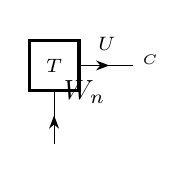
\begin{tikzpicture}[
    baseline=(current bounding box.center),
    leg2/.style={
      line width=1.1pt,
      postaction={
        decorate,
        decoration={
          markings,
          mark=at position 0.7 with {\arrow{Stealth[scale=1.0, fill=black]}}
        }
      }
    },
    leg/.style={
        postaction={decorate},
        decoration={
            markings,
            mark=at position 0.55 with {\arrow[scale=1.0]{Stealth}}
        }
    },
    tensor/.style={
      draw=black,
      fill=white,
      line width=1.1pt,
      minimum size=18pt,
      inner sep=2pt,
      rectangle
    }
  ]
    

  \begin{scope}
    \node[tensor] (T1) at (0,0) {\scriptsize $T$};

    \draw[leg] (0,-1) -- (T1.south) node[right] {$W_n$};
    
    \draw[leg] (T1.east) -- (1,0) node[right, yshift=2pt] {\tiny $C$} node[midway, above=2pt] {\scriptsize $U$};        
  \end{scope}

\end{tikzpicture}

If we have two tensors with matching legs, we can contract them by repeated application of the \emph{evaluation map}
\[
  V \otimes V^\ast \to k, \quad v \otimes f \mapsto f(v).
\]
and \emph{coevaluation} map
\[
  k \to V^\ast \otimes V, \quad \lambda \mapsto \sum_{i}^{} \lambda v_i \otimes f_i .
\]

The contraction operator $\mathcal{C}$ is then defined as the linear operator that \" removes \" the specified spaces from the product. As an example, the matmul between operators $A : U \otimes V^\ast$ and $B : V \otimes U^\ast$ is defined as
\[
  (\id_V \otimes \ev_{W} \otimes \id_{U^\ast})(- \otimes -) : (V \otimes W^\ast, W \otimes U^\ast) \to V \otimes U^\ast
\]

\newcommand{\mcT}{\mathcal{T}}

The article by \textcite{Penrose1971Applications} "Applications of Negative
Dimensional Tensors" introduces a \emph{string calculus} onto the theory of
tensors, however it also provides a formalization of a more general tensor
calculus over \emph{Abstract Tensor Systems (ATS)} by introducing a hierachy of
\emph{modules}
\[
  (\mcT, \mcT^a, \mcT^b, \ldots, \mcT_a, \mcT_b, \ldots, \mcT_b^a, \ldots, \mcT^{xm}_p, \ldots.)
\]
modeling processes in the ground field $\mcT$, the tensors with one incoming leg
$\mcT^a$, and outgoing leg $\mcT_a$ and combinations thereof.

These modules ought to be closed under certain operations:
\begin{itemize}
  \item[]addition : 
  \[
    + : \mcT^{x\ldots z}_{u\ldots w} \times \mcT^{x\ldots z}_{u\ldots w} \to \mcT^{x\ldots z}_{u\ldots w} 
  \]
  \item[]tensoring: 
  \[ 
    \ot : \mcT^{a\ldots d}_{p \ldots r} \times \mcT^{x\ldots z}_{u\ldots w} \to \mcT^{a\ldots d x\ldots z}_{p\ldots r u\ldots w} 
  \]  
  \item[] contraction:
  \[
    \mathcal{C}^p_q : \mcT^{px\ldots z}_{qu\ldots w} \to \mcT^{x\ldots z}_{u\ldots w}  
  \]
\end{itemize}

\begin{enumerate}
  \item[(A1)] {Addition forms an Abelian group}:
  \[
    S + T = T + S, \qquad S,T \in \mcT^{x\ldots z}_{u\ldots w}
  \]

  \[
    (S+T)+U = S+(T+U), \qquad S,T,U \in \mcT^{x\ldots z}_{u\ldots w}
  \]

  \[
    T + 0 = T, \qquad \forall\, T \in \mcT^{x\ldots z}_{u\ldots w}
  \]

  \item[(T1)] {Tensoring distributes over addition} (bilinearity of
  $\otimes$):
  \[
    (S+T)\otimes U = S\otimes U + T\otimes U, \qquad
    U \otimes (S+T) = U\otimes S + U\otimes T
  \]

  \item[(T2)] {Associativity of tensoring}:
  \[
    (S \otimes T) \otimes U = S \otimes (T \otimes U)
  \]

  \item[(C1)] {Contraction distributes over addition} (linearity of
  $\mathcal{C}^p_q$):
  \[
    \mathcal{C}^p_q(S + T) = \mathcal{C}^p_q(S) + \mathcal{C}^p_q(T)
  \]

  \item[(C2)] {Contractions are abelian} (independent contractions
  commute):
  \[
    \mathcal{C}^p_q \, \mathcal{C}^r_s = \mathcal{C}^r_s \, \mathcal{C}^p_q,
    \qquad p,q,r,s \ \text{distinct indices}
  \]

  \item[(C3)] {Contraction is local under tensoring}: if $p,q$ are
  indices belonging only to $S$,
  \[
    \mathcal{C}^p_q(S \otimes T) = \mathcal{C}^p_q(S) \otimes T
  \]
\end{enumerate}

\section{Some notation}
\newpage

\chapter{Symmetric Tensor Networks}
\label{sect:symmetricTensorNetworks}
This section develops the theory underlying \emph{symmetric tensor networks}, specifically
for nonabelian groups. We give an informal overview on the necessary representation
theoretic concepts in \Cref{sym:sub:rep}. We employ the example of the $XXZ$-Hamiltonain
for both abelian and anabelian symmetries and give an exact calculation of its conserved
values. Here we are mostly interested in the \emph{speedup} obtained by exploiting the
emergend block-structure of symmetric operators. Most of the proofs and formal definitions
required for this formalism are delegated to \Cref{sect:Categories}, however there will
still be repetitions of some of the theory.



\section{Representation theory}\label{sym:sub:rep}

In the following and the entire section, let $G$ be a compact group and $V,W$ be finite
dimensional vector spaces. We mainly follow the textbook by \textcite{woit2016}.

\begin{definition}[Representation]
  A \green{\emph{representation}} of a compact group $G$ over a vector space $V$ is a
  group homomorphism
  \[
    \rho : G \to \GL V, \quad \rho(g)\rho(h) = \rho(g \cdot h), \quad \rho(e) = id_V
  \]
  The \green{\emph{representation space}} is denoted by the tuple $(\rho, V)$ but usually
  we shorten this to just $V$.
\end{definition}

\noindent
Equivalently we can state the definition of a representation of $G$ as imposed by its
action on $V$, given as a map
  \begin{equation}
    \alpha : G \times V \to V, \quad (g,v) \mapsto g \cdot v
  \end{equation}
such that this is linear, todo. I think we get the equality to the hom def if we set $g \cdot v = \rho(g)v$

\begin{definition}[Intertwiner]
  A linear map $A : V \to W$ is an \emph{intertwiner}, if under representations $\rho_V :
  G \to \GL V$ and $\rho_W : G \to \GL W$ it holds that
  \[
    A \circ \rho_V(g) = \rho_W (g) \circ A \quad \forall g \in G.
  \]
  Denote the space of all intertwiners as $\Hom_G(V,W)$.
\end{definition}

\begin{definition}[Unitary representation]
  If our vector space $V$ is equipped  with a (Hermitian?) inner product 
\end{definition}

\begin{definition}[Irreducible representation (Woit 16)]
  A representation $\rho$ is an \emph{irrep} if there are no $W \subset V$ such that
  $(\rho_{\vert W}, W)$ is a representation. 
\end{definition}

\begin{definition}[Tensor product representation]
  \label{symm:def:tensor_product_representation}
  Given reps $(\rho_V, V)$ and $(\rho_W, W)$, the \emph{tensor product
  representation} $(\rho_{V\otimes W}, V \otimes W)$ is defined by its action on
  the elements
  \[
    \rho_{V \otimes W}(g) (v \otimes w) = \rho_V(g) v \otimes \rho_W(g) w
  \]
\end{definition}

\begin{definition}[Direct sum representation]
  As above, the \emph{direct sum representation} $(\rho_{V \oplus W}, V \oplus W)$ 
  \[
    \rho_{V \oplus W}(g) = \begin{pmatrix}
      \rho_V(g) &   \\
       &  \rho_W(g) \\
    \end{pmatrix}
  \]
\end{definition}

\begin{definition}[Isotypic / Semisimple decomposition]\label{sym:def:isotypic}
  Each semisimple representation $V$ decomposes as
  \[
    V \cong \bigoplus_{i \in I} V_i^{\oplus n_i} 
    \cong 
    \bigoplus_{i \in I} \C^{n_i} \otimes V_i
    \cong
    \bigoplus_{i \in I} V_i \otimes \C^{n_i}
  \]
  by grouping isomorphic simples. Is $n_i$ unique?
\end{definition}

Due to a theorem by Peter \& Weyl \cite{}, the unitary representations of any compact $G$ are
semisimple. 
%Therefore, for any representations $V$ and $W$ it holds that
%\[
%  V \otimes W \cong \bigoplus_{c \in I} R_c^{\oplus m_c} 
%\]
%where $m_c$ is determined uniquely (why intuitively?) in dependece on the decompositions of $V$ and $W$:
%\[
%  V \otimes 
%\]

Therefore, it must hold for any irreps $R_a,R_b$ of $G$ that their tensor product is
completely reducible with the decomposition
\[
  R_a \otimes R_b 
  \cong
  \bigoplus_{c \in I} R_c^{\oplus N_{ab}^c},
\]
with $N_{ab}^c$ called \emph{fusion-multiplicities}. If
\[
  N_{ab}^c \leq 1 \quad \forall a,b,c 
\]
the decomposition is said to be \emph{multiplicity-free}.

Note as well that the appearance of the \emph{direct sum} here (as discussed in
\cref{cat:eq:fusionprop}) is fully characterized (carefull how i phrase this) by its
injection and projection maps, for which we provide a graphical calculus.
\[
  \iota^{ab}_{c,\mu} : R_c \to R_a \otimes R_b \quad \text{ and } \quad \pi^{c,\mu}_{ab} : R_a \otimes R_b \to R_c \quad \text{ for } \mu \in 1,\ldots,N_{ab}^c  
\]
or alternatively
\[
  \ket{a,b;c,\mu} : R_c \to R_a \otimes R_b \quad \text{ and } \quad \bra{c,\mu; a,b} :R_a \otimes R_b \to R_c   
\]
\begin{equation}
\begin{tikzpicture}[
    baseline=(current bounding box.center),
    scale=1.0,
    string arrow/.style={
        postaction={decorate},
        decoration={
            markings,
            mark=at position 0.55 with {\arrow[scale=1.0]{Stealth}}
        }
    }
]
\begin{scope}[xshift=-1cm]

\coordinate (a) at (0,0.6);
\coordinate (b) at (1.2,0.6);
\coordinate (v) at (0.6,1.2);
\coordinate (c) at (0.6,2);

\draw[string arrow] (c) -- (v);
\draw[string arrow] (v) -- (a);
\draw[string arrow] (v) -- (b);

\node[below] at (a) {$R_a$};
\node[below] at (b) {$R_b$};
\node[above] at (c) {$R_c$};

\node[right=1pt] at (v) {$\mu$};

\end{scope}

\begin{scope}[xshift=4cm]

\coordinate (a) at (0,2);
\coordinate (b) at (1.2,2);
\coordinate (v) at (0.6,1.2);
\coordinate (c) at (0.6,0.4);

\draw[string arrow] (a) -- (v);
\draw[string arrow] (b) -- (v);
\draw[string arrow] (v) -- (c);

\node[above] at (a) {$R_a$};
\node[above] at (b) {$R_b$};
\node[below] at (c) {$R_c$};

\node[right=1pt] at (v) {$\mu$};

\end{scope}
\end{tikzpicture}
\end{equation}

These maps are more commonly known as \emph{clebsch-gordan coefficients}. Note that the
equations 
\begin{equation}
  \bra{\nu, d; a,b} \ket{a,b ; c,\mu} = \delta_{\mu \nu} \delta_{c d} \id_{R_c} 
\end{equation}
and 
\begin{equation}
  \sum_{c,\mu}^{} \ket{a,b;c,\mu}\bra{\mu,c; a,b} = \id_{R_a \otimes R_b}.
\end{equation}
As a consequence of this relation, the CG-tensors span the space $End(R_a \otimes R_b)$.

On the operators between tensor products, i.e. $T \in \End(R_a \otimes R_b)$ this yields a
formula
\[
  T \cong \bigoplus_c \id_{R_c} \otimes \; \C^{N_{ab}^c} 
\]

\begin{example}
  The simple objects of $G = \U{1}$ are given by the one-dimensional representations
  \[
    \chi_n : U(1) \to \C^{\times}, \quad e^{i\theta} \mapsto e^{i n \theta} 
  \]
  and each representation of $\U{1}$ decomposes as 
  \[
    V \cong \bigoplus_{n \in \Z} \chi_n^{\oplus m_n}. 
  \]
  It's fusion rule is given by
  \[
    \chi_n \otimes \chi_m = \chi_{n + m}
  \]
\end{example}

\begin{example}
  Let $G = \SU{2}$ and let $V_i$ and $V_j$ be two spin irreps of charge $i$ and $j$. These combine to
  \begin{equation}
    (\pi_{V_i \otimes V_{j}}, V_i \otimes V_j) = \bigoplus_{k \in \left\vert i - j \right\vert}^{i + j} (\pi_{V_k}, V_k) \label{sym:eq:cgseries}
  \end{equation}
  in what is referred to as the \emph{Clebsch-Gordan-series}.
\end{example}

\begin{example}[$\SU{2}$-CG tensors]
  Lets look at an example of spin irreps in the $\SU{2}$ theory. The combined basis of two
  spin-$\frac{1}{2}$ spaces is given by the collection $\{\ket{\uparrow},
  \ket{\downarrow}\}^{\otimes 2}$. By the fusion rule \cref{sym:eq:cgseries}, this
  decomposes as
  \[
    \frac{1}{2} \otimes \frac{1}{2} = 0 \oplus 1 
  \]
  with its accosiated basis $\{\ket{1,1},\ket{1,0},\ket{1,-1},\ket{0,0}\}$. The change of
  base tensors acting between these bases are precisely the Clebsch-Gordan tensors as
  defined in ???
\end{example}


% Just remove htis heading no? 
\section{Examples in symmetric hamiltonians.}

The motivation for constructing symmetric tensor networks is as follows: Assume we have a
(unitary) representation of a group $G$ denoted $U(g)$.  Furthermore assume we have a
hamiltonian that commutes with $[U(g)^{\otimes L}, H] = 0$. Then there are different
presentations of $H$ with respect to a certain basis by \emph{simulateneous
diagonalization}\cite[Thm~1.3.12]{Horn_Johnson_2012}, as shown in
\Cref{fig:diagonal_hamiltonians}. Notably these presentation induce a \emph{block-sparse}
structure on the respective operators. 

%If the ground state is unique,
%we can obtain 
%\[
%  U(g)^{\otimes L} H \ket{\psi_0} = H (U(g)^{\otimes L}) \ket{\psi_0} = E_0 U(g)^{\otimes L} \ket{\psi_0}
%\]
%and thus $U(g)\ket{\psi_{0} }$ is a ground state as well. By uniqueness
%\[
%  U(g) \ket{\psi_0} = e^{i\theta(g)} \ket{\psi_0}
%\]

\begin{figure}[h]
  \centering
  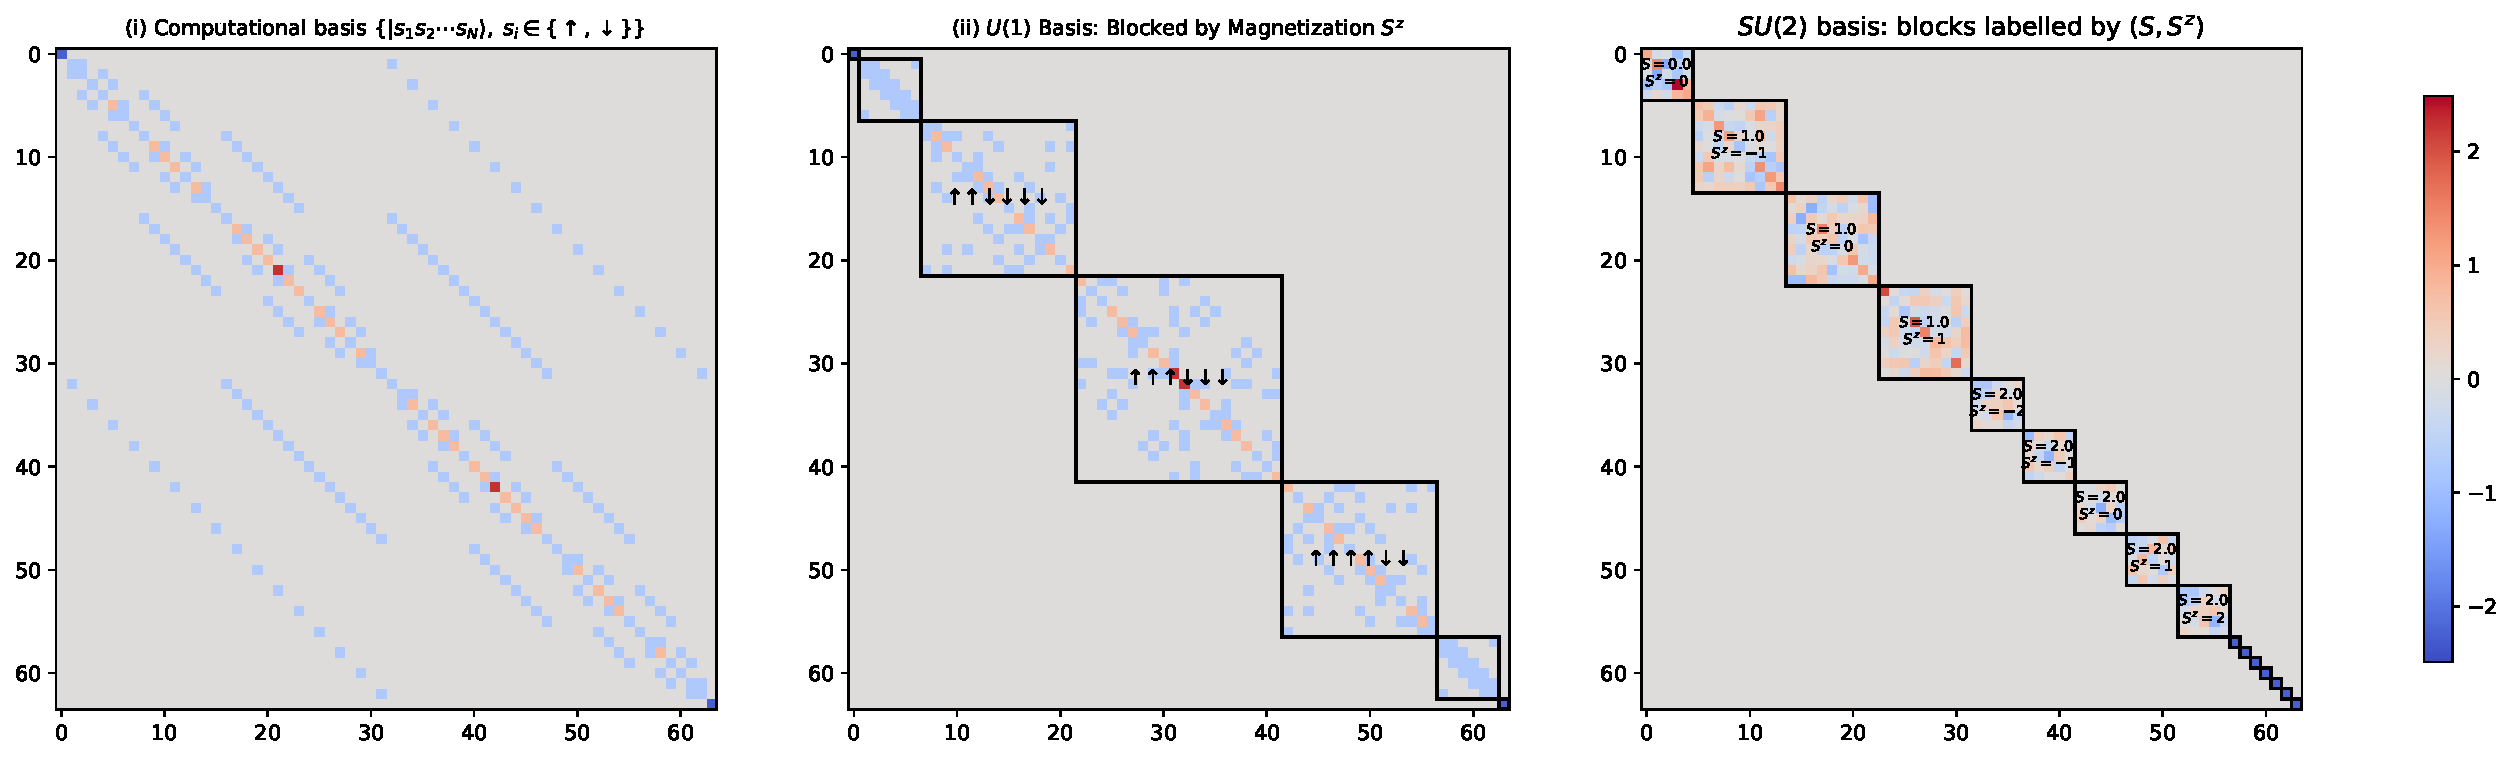
\includegraphics[width=\textwidth]{../experiments/plots/su2_block_structure.pdf}
  \caption{ Three different presentations of the XXZ Hamiltonian for $N = 6$. (i): In the default
    computational basis of spin vectors. (ii) In a reordering of the computational basis
    into equal spin up (down) classes, i.e. no spin up, one spin up etc..., here $U$ is
    simply a permutation matrix. (iii) After changing the basis into the $(S^2,S_Z)$
    basis. }
  \label{fig:diagonal_hamiltonians}
\end{figure}

We now show how to obtain this block-sparse structure and more by example of the $XXZ$ hamiltonian:

\begin{definition}\label{def:xxzHamiltonian}
  The \emph{\green{XXZ Hamiltonian}} on $N$ sites is
  \begin{equation}
    H 
    = 
    J \cdot 
    \sum_{i = 1}^{N-1}
      (\sigma_i^x \sigma_{i+1}^x + \sigma_i^y \sigma_{i+1}^y + \Delta \sigma_i^z \sigma_i^z  ),
  \end{equation}
  acting on the basis $\ket{s_1 s_2 \ldots s_n}$ where $s_i \in \{\uparrow, \downarrow\}$.
\end{definition}

This operator admits both a $\U{1}$ symmetry, and a $\SU{2}$ symmetry for $\Delta = 1$.
We elaborate on the (simpler) abelian case first:

The representations of $\U{1}$ here are induced by the operator
\[
  S^z_{\mathrm{tot}} = \frac12 \sum_{i = 1}^{N - 1} \sigma_i^z \quad \text{ with action } \quad U(\theta) : \theta \in \U 1 \mapsto e^{-i\theta S^z_{\mathrm{tot}}}
\]


It can be shown that $H$ is invariant under $U(\theta)$:
\begin{equation}\label{sym:eq:u1_commutes}
  U(\theta)HU(\theta)^\dagger \quad \underset{\text{suffices by \ref{app:proof:u1_commutes}}}{\iff} \quad  [H,S^z_{\mathrm{tot}}]=0.
\end{equation} % Something is weird with the reference here.

Diagonalizing both operators yields a block structure as in \Cref{fig:diagonal_hamiltonians}(ii). Note that change of base matrix in this case is given by a permutation matrix.

If we want to state this in terms of irreps, we have to realize that $\C^2 \cong \chi_{-1} \oplus \chi_1$. Then we can state the full space as
\[
  (\C^2)^{\otimes 6} \cong \chi_{-3} \oplus \chi_{-2}^6 \oplus \chi_{-1}^{\oplus 15} \oplus \chi_{0}^{\oplus 20} \oplus \chi_{1}^{\oplus 15} \oplus \chi_2^{\oplus 6} \oplus \chi_3 
\] 
and so we should expect $7$ blocks in total, just as given in \Cref{fig:diagonal_hamiltonians}.

%% Fine up until here.


In the $\SU 2$ case, we have the generators
\[
  S_{tot}^\alpha = \frac{1}{2} \sum_{i = 1}^{N} \sigma_i^\alpha, \quad \alpha \in \{x,y,z\} 
\]

The representation here is  $U(R) = e^{i\theta n \cdot S_{tot} }$ and the Hamiltonian is invariant under
\[
  U(R) H U(R)^\dagger = H, \quad R \in \SU 2
\]

Since
\[
  [S_{tot}^x, S_{tot}^y ] = i S_{tot}^z 
\]
we need a new operator for the simulatenous diagonalization
\[ 
  S_{tot} = \sum_{a \in \{x,y,z\}}^{} (S_{tot}^{a})^2
\]
and we need to verify this is indeed the correct operator TODO.

The eigenvalues of $S_{tot}^2$ are  $S(S + 1)$ where  $S$ are the half integers.

Again, we can solve this by diagonalizing all 3 operators? Do this calculation as in the .ipynb and put it in the appendix.

%%%
Or we can do the representation theoritical approach. Let $V_j$ denote the spin-$j$ irrep
of $\SU 2$. We have that $\C^2 \cong V_{\frac{1}{2}}$ and by \cref{sym:eq:cqseries} that
\[
  (\mathbb{C}^2)^{\otimes6} \cong V_{\frac{1}{2}}^{\otimes 6} \cong 5 V_0 \oplus 9V_1 \oplus 5V_2 \oplus V_3 \cong \C^5 \otimes V_{\frac{1}{2}} \oplus \C^9 \otimes V_0 \oplus \C^5 \otimes V_2 \oplus V_3
\]

Now our operator is a morphism in $End(V_{\frac{1}{2}}^{\otimes 6})$ and thus by Schurs
lemma\footnote{These are related by a permutation matrix. Proof? Is this the X from
\cite{devosTensorKitjlJuliaPackage2025}? We prefer the second presentation as this realizes more blocks.   }
\begin{equation}\label{sym:eq:blockdiag}
  H \in \bigoplus_{S \in 0,1,2,3} Mat_{m_S \times m_S} \otimes I_{2S+1} (\mathbb{C}) \cong \bigoplus_{S \in 0,1,2,3} I_{2S+1} \otimes Mat_{m_S \times m_S}(\mathbb{C}) 
\end{equation}

So we expect 20 blocks? 
$5$ have dimension $1$, $9$ have dimension $3$, $5$ have dimension $5$ and $1$ has $7$.

To get an interpretation of the matrix coefficients in $\eqref{sym:eq:cgseries}$, consider
a tiny Hamiltonian on $N = 2$ spins
\[
  H = \frac{J}{2} (\sigma_1^x \sigma_2^x + \sigma_1^y \sigma_2^y + \sigma_1^z \sigma_2^z)
  = J \cdot S_1 \cdot S_2
\]

This acts on the space $V_{\frac{1}{2}} \otimes V_{\frac{1}{2}}$ and thus on the basis
$\{\ket{\uparrow},\ket{\downarrow}\}^{\otimes 2}$ This has two distinct fusion outcomes,
$V_0$ and $V_1$. The basis on the rhs is given by
$\ket{1,1},\ket{1,0},\ket{1,-1}$ and $\ket{0,0}$, and we want to reformulate $S_1 \cdot S_2$ in
the total spin basis. Lets unfold this definition by 
\[
  S^2 = S_1^2 + S_2^2 + 2(S_1 \cdot S_2) \implies S_1 \cdot S_2 = \frac{1}{2}(S^2 - S_1^2 - S_2^2).
\]
Since $S_i^2 = s(s+1)$ is fixed for $s = \frac{1}{2}$ here, we ought to write
\[
  H = \frac{J}{2}(S^2 - 3/2)
\]
and this again splits into the sectors for $S = 0$ and $S = 1$
\[
  c_0 = \frac{J}{2}(0 - 3/2) = -\frac{3}{4}J
  \quad \text{ and } \quad
  c_1 = \frac{J}{2}(2 - 3/2) = \frac{1}{4}J
\]
which are exactly the two degrees of freedom we get by the direct sum. So we
expect our operator to look like
\[
  \begin{pmatrix}
    -3/4J &  0 \\
    0 &  \id_3 \otimes 1/4J \\
  \end{pmatrix}.
\]

By direct isomorphism\todo{meaningless phrasing}, we can write this as an element of $\End{V_{1/2}^{\ot 2}}$ \emph{factored} through its fusion result:
\begin{equation}\label{sym:eq:S1S2}
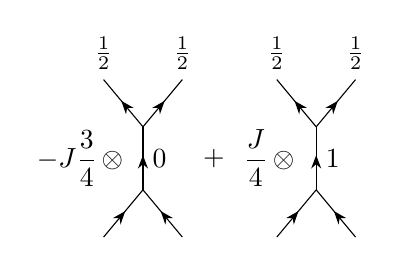
\begin{tikzpicture}[
    baseline=(current bounding box.center),
    scale=1.0,
    string arrow/.style={
        postaction={decorate},
        decoration={
            markings,
            mark=at position 0.55 with {\arrow[scale=1.0]{Stealth}}
        }
    }
  ]
  
  \node at (0.8,2.0) {$\displaystyle -J\frac{3}{4}\,\otimes$};
  \coordinate (bot_a) at (1.1, 1.0);
  \coordinate (bot_b) at (2.1, 1.0);
  

  \coordinate (mid_bot) at (1.6, 1.6);
  \coordinate (mid_top) at (1.6, 2.4);
  
  \coordinate (top_a) at (1.1, 3.0);
  \coordinate (top_b) at (2.1, 3.0);

  \draw[string arrow] (bot_a) -- (mid_bot);
  \draw[string arrow] (bot_b) -- (mid_bot);
  
  \draw[string arrow] (mid_bot) -- (mid_top) node[right, pos=0.5] {$0$};
  
  \draw[string arrow] (mid_top) -- (top_a) node[above] {$\frac{1}{2}$};
  \draw[string arrow] (mid_top) -- (top_b) node[above] {$\frac{1}{2}$};
  
  \node at (2.5, 2.0) {$+$};

\begin{scope}[shift={(2.2,0.0)}]
  \node at (1.0,2.0) {$\displaystyle\frac{J}{4}\,\otimes$};
  \coordinate (bot_a) at (1.1, 1.0);
  \coordinate (bot_b) at (2.1, 1.0);
  
  \coordinate (mid_bot) at (1.6, 1.6);
  \coordinate (mid_top) at (1.6, 2.4);
  
  \coordinate (top_a) at (1.1, 3.0);
  \coordinate (top_b) at (2.1, 3.0);


  \draw[string arrow] (bot_a) -- (mid_bot);
  \draw[string arrow] (bot_b) -- (mid_bot);
  
  \draw[string arrow] (mid_bot) -- (mid_top) node[right, pos=0.5] {$1$};
  
  \draw[string arrow] (mid_top) -- (top_a) node[above] {$\frac{1}{2}$};
  \draw[string arrow] (mid_top) -- (top_b) node[above] {$\frac{1}{2}$};
\end{scope}

\end{tikzpicture}
\end{equation}

Now we consider the same hamiltonian with $N = 3$, our ground state is
\[
  V_{1/2}^{\ot 3} = V_{3/2} \op V_{1/2} \op V_{1/2}
\]
with a multiplicity $2$ on the $1/2$ state and the Operator is
\[
  H = \frac{1}{2} (S_1 \cdot S_2 + S_2 \cdot S_3)
\]

\noindent
\begin{minipage}{0.65\textwidth}
\begin{align*}
S_1 \cdot S_2 
&=
\underbrace{\id_{V_{1/2}}}_{\dim 2}
\otimes
\begin{pmatrix}
  1/4 & 0  \\
  0 & -3/4
\end{pmatrix} 
\oplus
\underbrace{\id_{V_{3/2}}}_{\dim 4}
\otimes
(1/4) \\[0.8em]
S_2 \cdot S_3
&=
\underbrace{\id_{V_{1/2}}}_{\dim 2}
\otimes
\begin{pmatrix}
  -\frac{1}{2} & \frac{\sqrt{3}}{4} \\
  \frac{\sqrt{3}}{4} & 0
\end{pmatrix}
\oplus
\underbrace{\id_{V_{3/2}}}_{\dim 4}
\otimes
(1/4)
\end{align*}
\end{minipage}%
\begin{minipage}{0.35\textwidth}
\centering
\includegraphics[width=0.7\linewidth]{../experiments/plots/su2_sz_block_structure_3.png}
\end{minipage}



Visually we can define the operators before and include the groung state in a
tree-like fashion:
\begin{equation}
  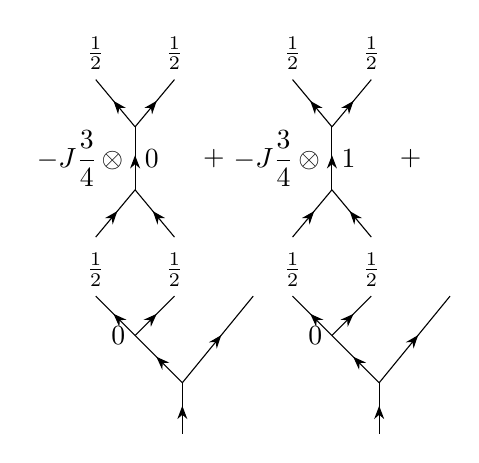
\begin{tikzpicture}[
    baseline=(current bounding box.center),
    scale=1.0,
    string arrow/.style={
        postaction={decorate},
        decoration={
            markings,
            mark=at position 0.55 with {\arrow[scale=1.0]{Stealth}}
        }
    }
  ]
  
  \coordinate (top_a) at (1.0, 1.0);
  \coordinate (top_b) at (2.0, 1.0);
  \coordinate (top_c) at (3.0, 1.0);
  
  \coordinate (mid_1) at (1.5, 0.5);
  \coordinate (mid_2) at (2.1, -0.1);

  \coordinate (bot_d) at (2.1, -0.75);

  \draw [string arrow] (bot_d) -- (mid_2);
  \draw [string arrow] (mid_2) -- (top_c);
  \draw [string arrow] (mid_2) -- (mid_1) node[left] {$0$};
  \draw [string arrow] (mid_1) -- (top_b) node[above] {$\frac{1}{2}$};
  \draw [string arrow] (mid_1) -- (top_a) node[above] {$\frac{1}{2}$};



  \begin{scope}[yshift=0.75cm]
    
  \node at (0.8,2.0) {$\displaystyle -J\frac{3}{4}\,\otimes$};
  \coordinate (bot_a) at (1.0, 1.0);
  \coordinate (bot_b) at (2.0, 1.0);
  

  \coordinate (mid_bot) at (1.5, 1.6);
  \coordinate (mid_top) at (1.5, 2.4);
  
  \coordinate (top_a) at (1, 3.0);
  \coordinate (top_b) at (2, 3.0);

  \draw[string arrow] (bot_a) -- (mid_bot);
  \draw[string arrow] (bot_b) -- (mid_bot);
  
  \draw[string arrow] (mid_bot) -- (mid_top) node[right, pos=0.5] {$0$};
  
  \draw[string arrow] (mid_top) -- (top_a) node[above] {$\frac{1}{2}$};
  \draw[string arrow] (mid_top) -- (top_b) node[above] {$\frac{1}{2}$};
  
  \node at (2.5, 2.0) {$+$};
  \end{scope}

  \begin{scope}[xshift = 2.5cm, yshift=0.75cm]
    
  \node at (0.8,2.0) {$\displaystyle -J\frac{3}{4}\,\otimes$};
  \coordinate (bot_a) at (1.0, 1.0);
  \coordinate (bot_b) at (2.0, 1.0);
  

  \coordinate (mid_bot) at (1.5, 1.6);
  \coordinate (mid_top) at (1.5, 2.4);
  
  \coordinate (top_a) at (1, 3.0);
  \coordinate (top_b) at (2, 3.0);

  \draw[string arrow] (bot_a) -- (mid_bot);
  \draw[string arrow] (bot_b) -- (mid_bot);
  
  \draw[string arrow] (mid_bot) -- (mid_top) node[right, pos=0.5] {$1$};
  
  \draw[string arrow] (mid_top) -- (top_a) node[above] {$\frac{1}{2}$};
  \draw[string arrow] (mid_top) -- (top_b) node[above] {$\frac{1}{2}$};
  
  \node at (2.5, 2.0) {$+$};

  \coordinate (top_a) at (1.0, 0.25);
  \coordinate (top_b) at (2.0, 0.25);
  \coordinate (top_c) at (3.0, 0.25);
  
  \coordinate (mid_1) at (1.5, -0.25);
  \coordinate (mid_2) at (2.1, -0.85);

  \coordinate (bot_d) at (2.1, -1.5);

  \draw [string arrow] (bot_d) -- (mid_2);
  \draw [string arrow] (mid_2) -- (top_c);
  \draw [string arrow] (mid_2) -- (mid_1) node[left] {$0$};
  \draw [string arrow] (mid_1) -- (top_b) node[above] {$\frac{1}{2}$};
  \draw [string arrow] (mid_1) -- (top_a) node[above] {$\frac{1}{2}$};

  \end{scope}


  \end{tikzpicture}
\end{equation}

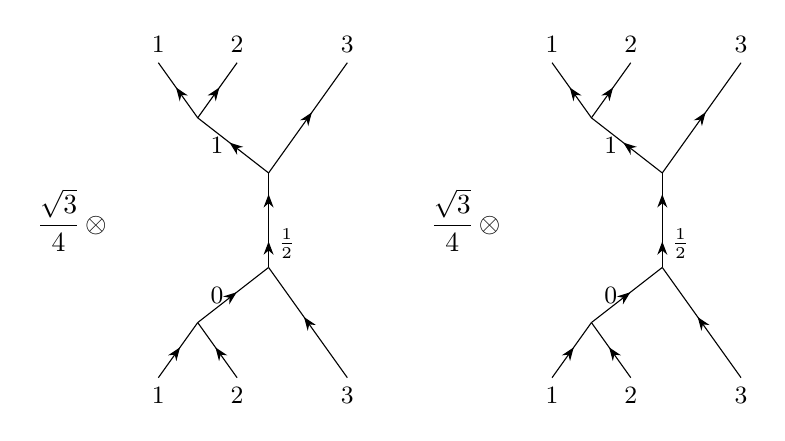
\begin{tikzpicture}[
    baseline=(current bounding box.center),
    string arrow/.style={postaction={decorate},
      decoration={markings, mark=at position 0.55 with {\arrow[scale=1.0]{Stealth}}}}
  ]
\node at (-1.1,2.0) {$\displaystyle\frac{\sqrt3}{4}\,\otimes$};
\coordinate (b1) at (0,0); \coordinate (b2) at (1,0); \coordinate (b3) at (2.4,0);
\coordinate (v1) at (0.5,0.7); \coordinate (v2) at (1.4,1.4); \coordinate (mid) at (1.4,2.0);
\draw[string arrow] (b1) -- (v1); \draw[string arrow] (b2) -- (v1);
\draw[string arrow] (v1) -- (v2) node[left,pos=0.5]{\small$0$};
\draw[string arrow] (b3) -- (v2);
\draw[string arrow] (v2) -- (mid) node[right,pos=0.5]{\small$\frac12$};

\coordinate (v2t) at (1.4,2.6); \coordinate (v1t) at (0.5,3.3);
\coordinate (t1) at (0,4.0); \coordinate (t2) at (1,4.0); \coordinate (t3) at (2.4,4.0);
\draw[string arrow] (mid) -- (v2t);
\draw[string arrow] (v2t) -- (v1t) node[left,pos=0.5]{\small$1$};
\draw[string arrow] (v2t) -- (t3);
\draw[string arrow] (v1t) -- (t1); \draw[string arrow] (v1t) -- (t2);

\node[below] at (b1) {\small 1}; \node[below] at (b2) {\small 2}; \node[below] at (b3) {\small 3};
\node[above] at (t1) {\small 1}; \node[above] at (t2) {\small 2}; \node[above] at (t3) {\small 3};

\begin{scope}[xshift=5.0cm]
  \node at (-1.1,2.0) {$\displaystyle\frac{\sqrt3}{4}\,\otimes$};
\coordinate (b1) at (0,0); \coordinate (b2) at (1,0); \coordinate (b3) at (2.4,0);
\coordinate (v1) at (0.5,0.7); \coordinate (v2) at (1.4,1.4); \coordinate (mid) at (1.4,2.0);
\draw[string arrow] (b1) -- (v1); \draw[string arrow] (b2) -- (v1);
\draw[string arrow] (v1) -- (v2) node[left,pos=0.5]{\small$0$};
\draw[string arrow] (b3) -- (v2);
\draw[string arrow] (v2) -- (mid) node[right,pos=0.5]{\small$\frac12$};

\coordinate (v2t) at (1.4,2.6); \coordinate (v1t) at (0.5,3.3);
\coordinate (t1) at (0,4.0); \coordinate (t2) at (1,4.0); \coordinate (t3) at (2.4,4.0);
\draw[string arrow] (mid) -- (v2t);
\draw[string arrow] (v2t) -- (v1t) node[left,pos=0.5]{\small$1$};
\draw[string arrow] (v2t) -- (t3);
\draw[string arrow] (v1t) -- (t1); \draw[string arrow] (v1t) -- (t2);

\node[below] at (b1) {\small 1}; \node[below] at (b2) {\small 2}; \node[below] at (b3) {\small 3};
\node[above] at (t1) {\small 1}; \node[above] at (t2) {\small 2}; \node[above] at (t3) {\small 3};
\end{scope}
\end{tikzpicture}






\section{Symmetric Tensors}

%Here we want to define tensors that are invariant under a symmetry $G$ (a compact group). We say that a tensor $T \in ()

Let $G$ be a compact group. Consider a tensor $T$ living in the tensor product
space of its legs:
\[
  T \in V_1 \otimes \cdots \otimes V_n \otimes W_m^\ast \otimes \cdots \otimes W_1^\ast
\]

Let $\rho_i : G \to \GL{V_i}$ be the linear representation of $G$ on each vector
space $V_i$, and let $\sigma_j^\ast : G \to \text{GL}(W_j^\ast)$ be the dual
representation on $W_j^\ast$. 

The total action of the group $G$ on the entire tensor product space is given by
\begin{gather*}
  \Pi: G \to \text{GL}\left(\bigotimes_i V_i \otimes \bigotimes_j W_j^\ast\right) \\
  \Pi(g) = \rho_1(g) \otimes \cdots \otimes \rho_n(g) \otimes \sigma_m^\ast(g) \otimes \cdots \otimes \sigma_1^\ast(g)
\end{gather*}


A tensor $T$ is defined to be a \textbf{symmetric tensor} (or $G$-invariant
tensor) if it is invariant under simultaneous action on all legs for all $g \in
G$ \cite{singhTensorNetworkDecompositions2010a}:
\[
  \Pi(g) T = T \quad \forall g \in G
\]

Recall that by the isomorphism $\Hom(V,W) \cong W \otimes V^\ast$ as
\[
  w \otimes f \mapsto (v \mapsto f(v)w).
\]
We can push the product representation through this isomorphism as
\begin{equation}\label{sym:eq:pushThrough}
   \pi(g)(w \otimes f) = \rho_W(g)w \otimes \rho_{V^\ast}(g)f = \rho_W(g)w \otimes (\rho_V(g)^{-1})^T  f = \rho_W(g)w \otimes f(\rho_V(g)^{-1} )
\end{equation}
 

\[
  \cong v \mapsto f(\rho_V(g)^{-1}v ) \rho_W(g)w
\]

By interpreting $T$ as a map
\[
  T : W_1 \otimes \cdots \otimes W_m \to V_1 \otimes \cdots \otimes V_n
\]
it follows directly from the definition of global invariance that the tensor must commute with the group action and we get the following definition of a symmetric tensor:

\begin{definition}
  \label{def:symmetricTensor}
  A \green{\emph{symmetric tensor}} is an intertwiner of the representations of the group $G$:
  \[
    \bigotimes_{j=1}^m \sigma_j(g) \circ T = T \circ  \bigotimes_{i=1}^n \rho_i(g) \quad \forall g \in G,
  \]
  which we denote by
  \[
    T \in Hom_G(W,V).
  \]
\end{definition}

\[
\begin{array}{c}
  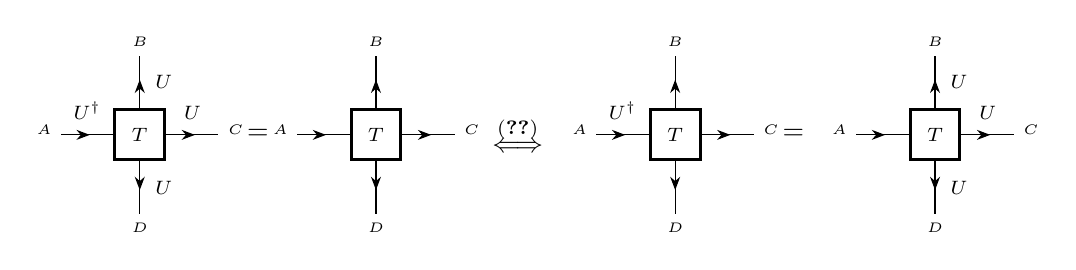
\begin{tikzpicture}[
    baseline=(current bounding box.center),
    leg2/.style={
      line width=1.1pt,
      postaction={
        decorate,
        decoration={
          markings,
          mark=at position 0.7 with {\arrow{Stealth[scale=1.0, fill=black]}}
        }
      }
    },
    leg/.style={
        postaction={decorate},
        decoration={
            markings,
            mark=at position 0.55 with {\arrow[scale=1.0]{Stealth}}
        }
    },
    tensor/.style={
      draw=black,
      fill=white,
      line width=1.1pt,
      minimum size=18pt,
      inner sep=2pt,
      rectangle
    }
  ]
    

  \begin{scope}
    \node[tensor] (T1) at (0,0) {\scriptsize $T$};
    \draw[leg] (-1,0) node[left, yshift=2pt] {\tiny $A$} -- (T1.west) node[midway, above=2pt] {\scriptsize $U^\dagger$}; 
    \draw[leg] (T1.north) -- (0,1) node[above] {\tiny $B$} node[midway, right=2pt] {\scriptsize $U$};        
    \draw[leg] (T1.south) -- (0,-1) node[below] {\tiny $D$} node[midway, right=2pt] {\scriptsize $U$};        
    \draw[leg] (T1.east) -- (1,0) node[right, yshift=2pt] {\tiny $C$} node[midway, above=2pt] {\scriptsize $U$};        
  \end{scope}

  \node at (1.5,0) {$=$};

  \begin{scope}[xshift=3.0cm]
    \node[tensor] (T2) at (0,0) {\scriptsize $T$};
    \draw[leg] (-1,0) node[left, yshift=2pt] {\tiny $A$} -- (T2.west);       
    \draw[leg] (T2.north) -- (0,1) node[above] {\tiny $B$};       
    \draw[leg] (T2.south) -- (0,-1) node[below] {\tiny $D$};      
    \draw[leg] (T2.east) -- (1,0) node[right, yshift=2pt] {\tiny $C$};        
  \end{scope}

  \node at (4.8,0) {$\overset{\eqref{sym:eq:pushThrough}}{\Longleftrightarrow}$};


  \begin{scope}[xshift=6.8cm]
    \node[tensor] (T3) at (0,0) {\scriptsize $T$};
    \draw[leg] (-1,0) node[left, yshift=2pt] {\tiny $A$} -- (T3.west) node[midway, above=2pt] {\scriptsize $U^\dagger$}; 
    \draw[leg] (T3.north) -- (0,1) node[above] {\tiny $B$};
    \draw[leg] (T3.south) -- (0,-1) node[below] {\tiny $D$};
    \draw[leg] (T3.east) -- (1,0) node[right, yshift=2pt] {\tiny $C$};
  \end{scope}

  \node at (8.3,0) {$=$};

  \begin{scope}[xshift=10.1cm]
    \node[tensor] (T4) at (0,0) {\scriptsize $T$};
    \draw[leg] (-1,0) node[left, yshift=2pt] {\tiny $A$} -- (T4.west);                  
    \draw[leg] (T4.north) -- (0,1) node[above] {\tiny $B$} node[midway, right=2pt] {\scriptsize $U$};        
    \draw[leg] (T4.south) -- (0,-1) node[below] {\tiny $D$} node[midway, right=2pt] {\scriptsize $U$};        
    \draw[leg] (T4.east) -- (1,0) node[right, yshift=2pt] {\tiny $C$} node[midway, above=2pt] {\scriptsize $U$};        
  \end{scope}
  \end{tikzpicture}\\[2.0em]
  
  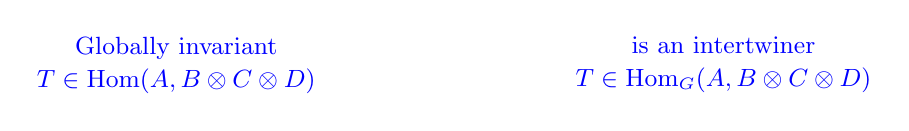
\begin{tikzpicture}[baseline=(current bounding box.center)]
    \node[anchor=north, align=center, text=blue] at (1.5,0) {
      \small Globally invariant \\
      \small $T \in \operatorname{Hom}(A, B \otimes C \otimes D)$
    };
    
    \node[anchor=north, align=center, text=blue] at (8.45,0) {
      \small is an intertwiner \\
      \small $T \in \operatorname{Hom}_G(A, B \otimes C \otimes D)$
    };
  \end{tikzpicture}
\end{array}
\]

\begin{corollary}[Networks of symmetric tensors are symmetric]
  Since a tensor network is built by composition and application of the $(co)ev$ maps,
  both of which are intertwiners, the full network is also an intertwiner. Important there
  is that this entire discussion is only about FdVect or FdHilb for now, but i think the
  same applies to any braided category.    
\end{corollary}


\begin{definition}\label{def:MPS}
  A \emph{\green{Matrix Product State}} is a quantum state $\ket{\psi}$ with $n$ legs written as
  the contraction of $n$ trivalent tensors $\{A^{[i]}\}_{i \in [n]}$. Formally this reads
  \[
    \ket{\psi[A]}
    =
    \sum_{i_1,\ldots,i_n}
    \operatorname{Tr}\!\left(
    A^{[1]}_{i_1}
    A^{[2]}_{i_2}
    \cdots
    A^{[n]}_{i_n}
    \right)
    \ket{i_1i_2\cdots i_n},
  \]
  where $A^{[i]}_{i_{k}} \in \mathbb{C}^{D_i \times D_{i+1} }$. The elements of the
  collection $\{D_i\}_{i \in [n]}$ is referred to as the \emph{\green{bond-dimensions}}.
\end{definition}
Note that this is a state with closed boundaries. If we want open boundaries we have to
replace the trace with appropriate end vectors (nice source?).

\begin{example}
  We can represent each product state $\ket{\varPsi} = \ket{\psi}^{\otimes n}$ as a MPS with bond dimension $1$.
\end{example}

\begin{theorem}[Fundamental Theorem of MPS]
  If two MPS states generated by $A$ and $B$ respectively.
  Figure out what we can do with this. 
  
  Proof \cite{ciracMatrixProductDensity2017},\cite{vercleyenMathematicalStructureTensor2018}, \cite{perez-garciaStringOrderSymmetries2008a}.
\end{theorem}

\subsection{Algorithms for block-sparse
tensors}\label{sym:sec:algorithms_for_block_sparse_tensors}
\newpage

% TODO: fix
\chapter{Anyons I : Introduction}
\label{sec:anyonsIntro}
This chapter introduces the theory of anyons by a set of physical requirements.
The algebraic definition of anyons will then by given by the discussion in
\Cref{sect:Categories}.

Anyons are proposed as a \emph{defect} in a $2$ dimensional space (manifold?
compact?) with \emph{exotic exchange statistics}. These exchange statistics
differ from bosons or fermions in that we allow particles to pick up a arbitrary
phase $e^{i\theta}$ on exchange in the abelian case, and a phase as a matrix
element in the nonabelian case.

We group anyons into theories. An anyon theory carries a finite set of charges
(types) $a,b,c\ldots$ including a trivial \emph{vacuum} charge. We are then
interested in their spacetime histories, as this is where the topological
properties of the anyon become apparent. First fix an oriented manifold $D$ of
dimension two as our base space. Then introduce an anyonic defect as a point
like hole (that is also oriented), that is carrying a charge. Such a particles
spacetime history is then given by an appropriate 3-manifold.\todo{I dont like
this whole section.}

\section{Configuration Spaces \& The Braid Group}
\label{sect:anyons1:configurations_spaces_and_the_braid_group}

The original article by \textcite{leinaasTheoryIdenticalParticles1977a}
identifies a generalized theory of \emph{identical} particles. Denote the space
where a particle lives by $\Sigma$ and thus the space of $n$ particles possible
coordinates of equal type by $\Sigma^n \coloneqq \bigtimes^n \Sigma$. Since the
particles are assumed to be identical, any permutation (an action of $S_n$)
necessarily leads to the same physical state, so we denote the full space of our
system by the quotient
\[
    \Sigma^n / S_n.
\] 
However we also want no two particles occupying the same space\footnote{If this
were the case, then the resulting exchange statistics would be bosonic
\cite[Footnote~12]{wuGeneralTheoryQuantum1984}.}, so the diagonal in $\Delta =
\{x \in \Sigma^n \mid x_i = x_j \text{ for some } i \neq j\}$\todo{rephrase!}
needs to be excluded as well \cite{wuGeneralTheoryQuantum1984}. This leads to
the expression
\[
    \uConf_n(\Sigma) = (\Sigma^n - \Delta) / S_n
\]  
which is defined to be the \emph{configuration space} of $n$ unordered
particles. However as we will see, anyons come in different "types", and we
consider only particles of the same type to be identical. Later publications
however define a swath of different notions of configuration spaces. We follow
\cite{satiDifferentialCohomotopyImplies2022}\todo{original publications.} with
the following definition:
\begin{definition}
    The \emph{\green{ordered Configuration Space}} of $n$ particles of possibly
    differnt types (or labeled particles with the same type) on a surface of
    dimension $D$ is
    \[
        \oConf n (\Sigma) := (\Sigma)^n - \Delta_{\Sigma}^n
    \] 
    and the \emph{\green{unordered Configuration Space}} of $n$ unlabeled
    identical particles is defined as 
    \[
        \uConf_n (\Sigma) := \oConf n (\Sigma) / S_n.
    \]
\end{definition}    

\begin{figure}
  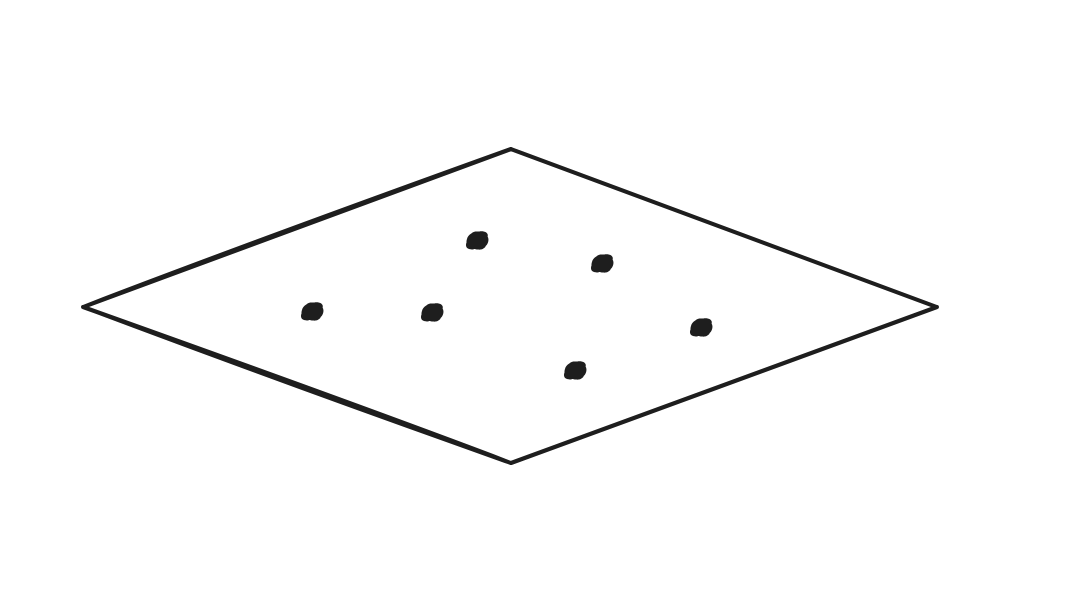
\includegraphics[width=0.5\textwidth]{figures/conf_5.png}
  \caption{The configuration space of 5 particles in the plane $\R^2$.}
\end{figure}

Note that while \cite{leinaasTheoryIdenticalParticles1977a} conjectured
computations for strange exchange statistics in both $2$ and $3$ dimensions, the
concept of an anyon as a $1$ dimensional representation is due to
\cite{wilczek1990}. 

Now we want to classify all the possible motions particles can take in this
space. The \emph{motion group} of the configuration space is given by the spaces
\emph{homotopy classes} (c.f. \Cref{app_gen:homotopy}), which are given by the
fundamental group(oid) of the spcae. Informally, this group collects all the
loops at some configuration $x_0$ up to homotopy. We want to differentiate two
cases here: If $D = 2$ it is known that

\[
    \pi_1(\uConf_n (\Sigma)) = \Br_n(\Sigma) \quad \text{ and } \quad \pi_1(\oConf{n} (\Sigma)) = \PBr_n(\Sigma)
\]
however if $D >= 3$ we know that both of these coincide with the symmetric group
$S_n$ instead. In fact there is an exact sequence
\[
    1 
    \longrightarrow 
    \mathrm{PBr}_n(\Sigma) 
    \longrightarrow 
    \mathrm{Br}_n(\Sigma)
    \longrightarrow 
    S_n 
    \longrightarrow 
    1 .
\]
For an example in the plane $\R^2$ (or $\C$?), we give an explicit
representation of the \emph{braid group} $\Br_n(\R^2)$ and the \emph{pure braid
group} $\PBr_n(\R^2)$. There is a well know presentation in terms of generators
due to \cite{artin25} as
\[
    \Br_n(\R^2)
    = 
    \left\langle
    \sigma_1, \ldots, \sigma_{n-1}
    \;\middle\vert\;
    \begin{aligned}
        \sigma_i\sigma_{i+1}\sigma_i &= \sigma_{i+1}\sigma_i \sigma_{i+1} \\
        \sigma_i\sigma_j &= \sigma_j\sigma_i,\; \vert i - j \vert \geq 2
    \end{aligned}
    \right\rangle.
\]
These generators also have a graphical interpretation as
\begin{equation}
\sigma_i
\;\coloneqq\;
\left[
\color{black}
\raisebox{-28pt}{
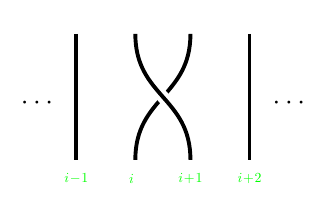
\begin{tikzpicture}[yscale=.8]

\begin{scope}[shift={(-1.6,0)}]
\draw[line width=1.4]
  (+.5,1) to (+.5,-1);
\draw
  (-0,-.1) node {$\mathclap{\cdots}$};
\end{scope}
\draw[line width=1.4]
  (-.35,-1)
  .. controls (-.35,0) and (+.35,0)  ..
  (+.35,1);

\draw[line width=4.5, white]
  (+.35,-1)
  .. controls (+.35,0) and (-.35,0)  ..
  (-.35,1);
\draw[line width=1.4]
  (+.35,-1)
  .. controls (+.35,0) and (-.35,0)  ..
  (-.35,1);
\begin{scope}[shift={(+1.6,0)}]
\draw[line width=1.4]
  (-.5,1) to (-.5,-1);
\draw
  (-0,-.1) node {$\mathclap{\cdots}$};
\end{scope}

\draw
  (-1.1, -1.3) node {\color{green}\scalebox{.5}{$i\!-\!1$}};
\draw
  (-.4, -1.3) node {\color{green}\scalebox{.5}{$i$}};
\draw
  (+.35, -1.3) node {\color{green}\scalebox{.5}{$i\!+\!1$}};
\draw
  (+1.1, -1.3) node {\color{green}\scalebox{.5}{$i\!+\!2$}};
\end{tikzpicture}
} 
\right]
\end{equation}

Now we can give a process as the \emph{spacetime history} diagram of the $n$ particles.

    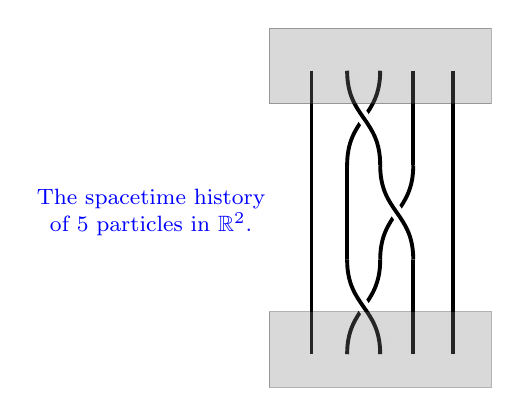
\begin{tikzpicture}
\begin{scope}[scale=0.6]
  \begin{scope}[shift={(-1.6,0)}]
    \draw[line width=1.2]
      (+.5,5) to (+.5,-1);
  \end{scope}

  \begin{scope}[shift={(0,4)}]
    \draw[line width=1.4]
      (-.35,-1)
      .. controls (-.35,0) and (+.35,0)  ..
      (+.35,1);

    \draw[line width=4.5, white]
      (+.35,-1)
      .. controls (+.35,0) and (-.35,0)  ..
      (-.35,1);
    \draw[line width=1.4]
      (+.35,-1)
      .. controls (+.35,0) and (-.35,0)  ..
      (-.35,1);
  \end{scope}

  \draw[line width=1.4]
    (-.35,3)
    --
    (-.35,1);

  \draw[line width=1.4]
    (+1.05,5)
    --
    (+1.05,3);

  \begin{scope}[shift={(.7,2)}]
    \draw[line width=1.4]
      (-.35,-1)
      .. controls (-.35,0) and (+.35,0)  ..
      (+.35,1);

    \draw[line width=4.5, white]
      (+.35,-1)
      .. controls (+.35,0) and (-.35,0)  ..
      (-.35,1);
    \draw[line width=1.4]
      (+.35,-1)
      .. controls (+.35,0) and (-.35,0)  ..
      (-.35,1);
  \end{scope}

  \begin{scope}
    \draw[line width=1.4]
      (-.35,-1)
      .. controls (-.35,0) and (+.35,0)  ..
      (+.35,1);

    \draw[line width=4.5, white]
      (+.35,-1)
      .. controls (+.35,0) and (-.35,0)  ..
      (-.35,1);
    \draw[line width=1.4]
      (+.35,-1)
      .. controls (+.35,0) and (-.35,0)  ..
      (-.35,1);
  \end{scope}

  \draw[line width=1.4]
    (1.05,1) to (1.05,-1);

  \begin{scope}[shift={(+2.4,0)}]
    \draw[line width=1.4]
      (-.5,5) to (-.5,-1);
  \end{scope}

  \draw[fill=gray, opacity=0.3] (-2,4.3) rectangle (2.7,5.9);

  \draw[fill=gray, opacity=0.3] (-2,-0.1) rectangle (2.7,-1.7);

  \node[align=center, blue, font=\footnotesize] at (-4.5, 2) 
        {The spacetime history \\ of $5$ particles in $\R^2$.};

  \end{scope}
\end{tikzpicture}

We can also do an example on there $2$-sphere, since there is an extra relation
of the $\R^2$ braid group. Generally, this braid group arises as a
\emph{quotient} of the Artin group, but this does not hold in general.

\begin{figure}[H]
  \centering
  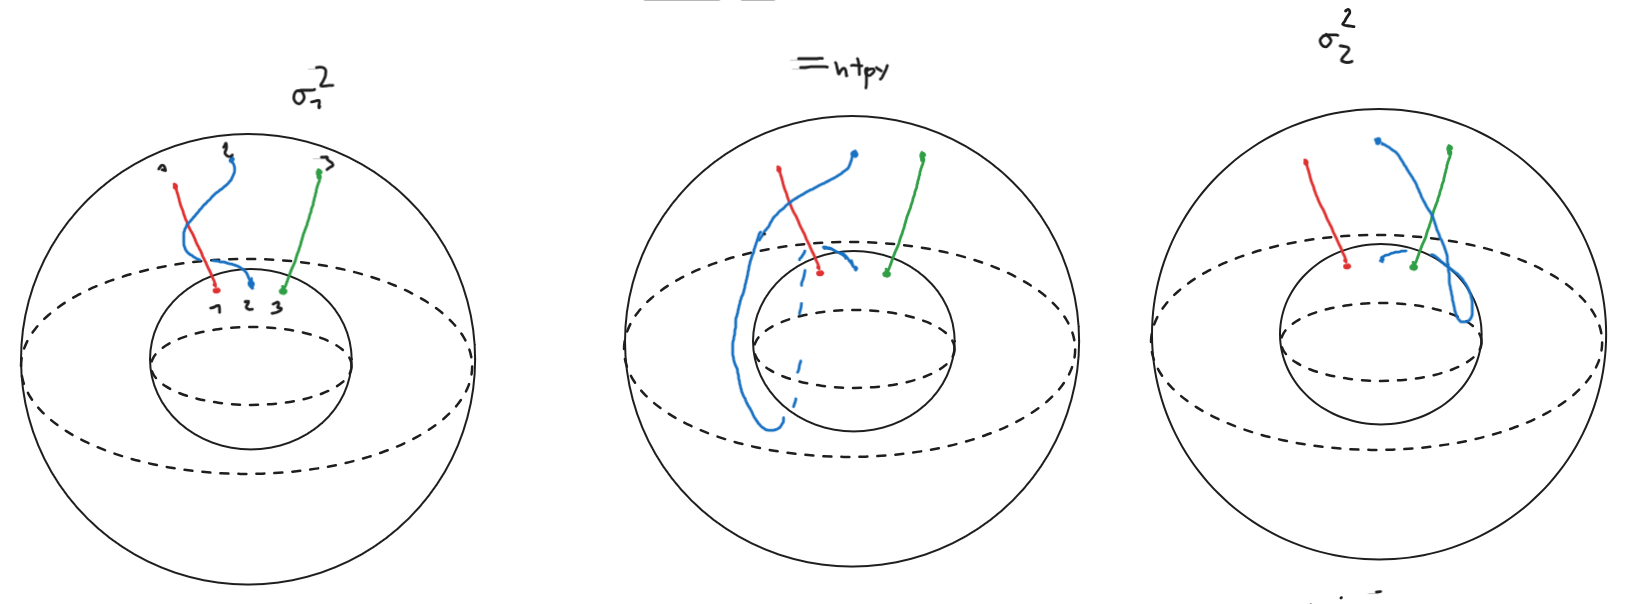
\includegraphics[width=0.8\textwidth]{figures/anyons_sphere.png}
  \caption{ $3$ Anyons on the sphere $S^2$ with the equivalence of the braids $\sigma_1^2$
    and $\sigma_2^2$. From an
    exercise\href{https://github.com/jkr11/maths-notes/tree/main/tq-simons-solutions}{github}
    in \cite{simonTopologicalQuantum2023}. }
  \label{anyon:fig:sphere}
\end{figure}

Analyzing this case further yields that 
\[
  \pi_1(\mathrm{Conf}_3(S^2)) \cong Br(S^2) \cong \Z_4 \boxtimes \Z_3
\]
and thus finite. In fact, we know about the braid group on spheres that the
order of $Br_n(S^2)$ is given by
\begin{equation}
  \left\vert Br_n(S^2) \right\vert = \begin{dcases}
    \left\vert \Z_2 \right\vert = 2 &\text{ if } n = 2,\\
    \left\vert ??? \right\vert = 12  &\text{ if } n = 3, \\
    \infty &\text{ if } n \geq 4.
  \end{dcases}
  %\text{
  %  \stackrel{\cite[P~255]{fadellBraidGroupsE21962}}{\cite[Prop~2.2]{nlab:spherical_braid_group}}
  %}
  \shortstack[l]{
    \cite[p.~255]{fadellBraidGroupsE21962} \\
    \cite[Prop~2.2]{nlab:spherical_braid_group}
  }
\end{equation}

Now, if we associate a Hilbert space to this configuration space, we can achieve
this by using a \emph{Hilbert Bundle}
\[
  \mathcal{H} \overset{\pi}{\longrightarrow} \oConf{n}(\Sigma),
\]
i.e. to each point $x \in \oConf{n}(\Sigma)$ there is an associated Hilbert
space $\mathcal{H}_{x}$. Furthermore, a path through the configuration space
$[\gamma] : x_0 \to x_1 \in \oConf{n}(\Sigma)$ is lifted to some unitary
representation
\[
  \rho([\gamma]) \in U(\mathcal{H}_{x_0} \to \mathcal{H}_{x_1})
\]
by \emph{parallel transport}.

The closed paths in the respective groups form a \emph{monodromy} in the
configuration space and a \emph{holonomy} in the Hilbert Bundle, and it is these
generators that yield us unitary gates that are universal for \emph{topological
quantum computation} (c.f. \Cref{sect:anyon:tqc})


However, in the usual literature anyons are also identified over their
\emph{fusion tensor category} (c.f. \Cref{sect:Categories}). Shifting the
viewpoint from configuration spaces to fusion categories requires additional
postulates \todo{is this true?} about the systems we want to reason about.
Although this correspondence is well known and the categorical interpretation
can be considered standard, a formal treatment and proof \todo{Check if htis is
a full proof.} were only given recently. These are pointed out in
\cite{valeraFusionStructureExchange2021}, and formally rigorous derivations of
this fact are given in \cite{satiAnyonicTopologicalOrder2023}. However we will
not give a derivation of this result and instead assume it. Perhaps a more
natural introduction to this correspondence is given by an excursion over MCGs
as done in \cite{burtonShortGuideAnyons2016}.

\chapter{Categorical Networks}
\label{sect:Categories}
In the existing literature it is well known that all of the concepts we have seen up to know are modeled by a formalism called \emph{tensor categories}:
\begin{enumerate}
  \item $\Veck$ and $\Hilb$ tensors are the most trivial and motivating case and
  trivial build tensor categories.
  \item $\Rep(G)$ (for $G$ finite) as in \cref{sect:symmetricTensorNetworks} are
  one of the primary motivations for construction fusion tensor categories.
  \cite{etingofFusionCategories2017}.
  \item All anyonic topological orders (i.e species of quasiparticles as in
  \cref{sect:anyons1:configurations_spaces_and_the_braid_group}) can be
  classified by \emph{modular tensor categories (MTCs)}
  \cite{kitaevAnyonsExactlySolved2006}\cite{rowellClassificationModularTensor2009}.
\end{enumerate}

\begin{literature}[Tensor Categories]
  Grothendieck investigated what we now know as tensor categories as part of a
  larger study on \emph{tannakian categories} to related the methods of
  representation theory (c.f. 3) to less related mathematical problems. Monoidal
  categories in turn were introduce by Benabou \cite{} and MacLane \cite{} under
  the name \emph{bicategory} and \emph{category with multiplication}, although
  an elementary construction of such categories is given by Tannaka \cite{} 

  The name \emph{tensor category} is due to \textcite{Deligne1990} in
  "Catégories Tannakiennes" and its followup
  \cite{deligneCategoriesTensorielles2002} \todo{there is one here from 1982
  find what this does.}
  BlaBlub

  The correspondence between the penrose notation (i.e. planar diagrams) and the
  calculus provdided by tensor categories is explained in great detail in
  \textcite{joyalGeometryTensorCalculus1991}, although earlier accounts such as
  \cite{reshetikhinInvariants3manifoldsLink1991} already make use of such a
  string calculus.


\end{literature}

We have also seen a method for evaluating networks built in $\Rep(G)$ in
\cref{sect:symmetricTensorNetworks} by decomposing a network into its fusion
tree and it's degneracy spaces. As an immedeate consequence, this yields an
algorithm for evaluating generalized \emph{anyonic} and \emph{categorical}
tensor networks, as in
\cite[§~4]{dissertation}\cite{devosTensorKitjlJuliaPackage2025}
\cite{pfeiferSimulationAnyonsUsing2012,pfeiferSimulationAnyonsTensor2010}
\cite{ayeniStudiesBraidedNonAbelian2017}
\cite[§~?]{schmollProgrammingGuideTensor2020}.

In light of this we provide a bottom-up construction of the theory of fusion
categories in \cref{cat:sub:introCat}, each concept will carry along an example
for representations, a physical interpretation in terms of anyonic
worldlines\todo{or tqfts?} as well as the correspondence to the ATS systems of
\textcite{Penrose1971Applications}. We formalize the aforementioned
decomposition in \cref{cat:sub:decomp} and list the algorithms necessary for
achieving a tensor network out of these theories.

If we however mention ATSs, it must be said that there is a multitude of
tensor-like string calculi and correspondences to categories. A great review of
these string like languages is given by
\textcite{selingerSurveyGraphicalLanguages2011}. Furthermore, the string
calculus as defined by penrose for the ATSs does not have an abstract
formulation that is sound and coherent as defined by
\cite{joyalGeometryTensorCalculus1991}. The definitions of these terms will be
given in the boxes labeled Graphical Notation.

\section{Tensor \& Fusion Categories}\label{cat:sub:introCat}

The general idea of a category is that it admits a sort of \emph{interface}. As
noticed, there are many similarities in data and structure between the entities
we already dealt with, i.e. the tensor product of vector space, the tensor
product of representations, of Hilbert spaces etc.... We can view all these
concepts as a category with additional constraints added.

\begin{definition}\label{cat:def:category} A \emph{\green {category}}
  $\mathcal{C}$ consists of\todo{Mention consisting of data?}
  \begin{itemize}
    \item a set of \emph{objects} $\mathrm{ob}(\mathcal{C})$,
    \item for every pair $A, B \in \mathrm{ob}(\mathcal{C})$, a \emph{hom-set}
    $\Hom_{\mathcal{C}}(A,B)$ of \emph{morphisms} $f : A \to B$,
    \item for every $A \in \mathrm{ob}(\mathcal{C})$, an \emph{identity
    morphism} $\id_A : A \to A$,
    \item for every triple $A,B,C \in \mathrm{ob}(\mathcal{C})$, a
    \emph{composition} map
    \[
      \circ \, : \, \Hom_\CC(B,C) \times \Hom_\CC(A,B) \longrightarrow \Hom_\CC(A,C),
    \]
  \end{itemize} such that composition is \emph{associative}, i.e.\ $(f \circ g)
  \circ h = f \circ (g \circ h)$ whenever defined, and \emph{unital}, i.e.\ $f
  \circ \mathrm{id}_A = f = \mathrm{id}_B \circ f$ for all $f : A \to B$.
\end{definition}

\begin{example}
  Some examples here:
  \begin{enumerate}
    \item The category $\Veck{}$ is the category of finite dimensional vector
    spaces and its morpisms are the linear operators between vector spaces.
    \item The category $\Hilb$ is the category whose objects are Hilbert spaces
    and whose morphisms are the bounded linear operators between them. Here we
    can alternatively take the objects to be the tuple $(\mathcal{H},
    \left\langle -, -\right\rangle)$.
    \item The category $\Set$ admits sets as objects and functions between sets
    as the morphisms.
    \item The product category $\CC \times \mathcal{D}$ holds as objects tuples
    $(a \in \CC, b \in \mathcal{D})$ and as morphisms tuples of maps $(f \in
    \Hom_\CC(a_1, a_2), g \in \Hom_\mathcal{D}(b_1, b_2))$.
  \end{enumerate}
\end{example}

We can take categories and associate them with each other by use of a
\emph{functor}.
\begin{definition}
  A \emph{\green{functor}} $F$ between the categories $\CC$ and $\CD$, denoted
  as $F : \CC \to \CD$ assigns to each object $A \in \CC$ an object $F(A) \in
  \CD$ as well as to every morphism in $f : A \to B \in \Hom_\CC$ a morphism
  $F(f) : F(A) \to F(B) \in \Hom_\CD$. Additionally, this must satisfy
  \[
    F(\id_A) = \id_{F(A)}
  \] as well as one of the cases 
  \begin{equation}
    F(g \circ f) = F(g) \circ F(f) \quad \text{ in the \emph{\green{covariant}} case}
  \end{equation}
  or 
  \begin{equation}
    F(g \circ f) = F(f) \circ F(g) \quad \text{ in the \emph{\green{contravariant}} case.}
  \end{equation}
\end{definition}

We can also relate functor with each other through maps between them. An
important relation here will be \emph{naturality}:
\begin{definition}
  A transformation $\tau$ between functors $F,G : \CC \to \CD$ is
  \emph{\green{natural}} if the diagram commutes for all $A : \ob(\CC)$ and $f :
  \Hom_\CC(A,B)$:
  % https://q.uiver.app/#q=WzAsNCxbMCwwLCJGKEEpIl0sWzIsMCwiRyhBKSJdLFswLDIsIkYoQikiXSxbMiwyLCJHKEIpIl0sWzEsMywiRyhmKSJdLFswLDIsIkYoZikiXSxbMCwxLCJcXHRhdV9BIl0sWzIsMywiXFx0YXVfQiJdXQ==
  \[\begin{tikzcd} {F(A)} && {G(A)} \\
	  \\
	  {F(B)} && {G(B)}
	  \arrow["{\tau_A}", from=1-1, to=1-3]
	  \arrow["{F(f)}", from=1-1, to=3-1]
	  \arrow["{G(f)}", from=1-3, to=3-3]
	  \arrow["{\tau_B}", from=3-1, to=3-3]
  \end{tikzcd}\]
\end{definition}

\begin{example}
  As an immedeate appliation, consider the category of Hilbert spaces $\Hilb$
  and assign it a \emph{forgetfull} functor $\omega : \Hilb \to \Veck$ that
  takes each Hilbert space to its underlying vector space, and each bounded
  linear operator to its linear operator between vector spaces.
\end{example}

%We want to embed some of the larger structures of $\Rep(G)$ and $\VecCat{\C}$
%into the categorical formalism. For fdVect, the hom spaces of linear maps $V
%\to W$ have a natural identification as a vector space as well. The composition
%map is $\C$-bilinear. This immedeately motivates the following definition:
%
%\begin{definition}\label{cat:def:clinear} A \green{\emph{$\C$-linear category}}
%  \todo{Check if we need enrichment.} endows each of its hom-sets with a module
%  structure, such that the composition is bilinear. That is
%  \[
%    \circ \, : \, \Hom_\mathcal{C}(B,C) \times \Hom_\mathcal{C}(A,B) \longrightarrow \Hom_\mathcal{C}(A,C)
%  \]
%  is $\C$-bilinear: for all $f, f' : B \to C$, \,\, $g, g' : A \to B$, and $c
%  \in \C$,
%  \[
%    (f + f') \circ g = f \circ g + f' \circ g, \qquad
%    f \circ (g + g') = f \circ g + f \circ g', \qquad
%    (cf) \circ g = c(f \circ g) = f \circ (cg).
%  \]
%\end{definition}
%
We will now explore how to use category theory to model quantum processes. We want this to
be able to do a list of things. First, given two systems $A$ and$B$, we want the combined
system to be an object as well. Given processes, i.e. operators on each individual system
$f : A \to A^\prime$,$g : B \to B^\prime $, there should be a combined process.
Additionally, structures such as entanglement and no-cloning should be readily apparent in
this theory.

\todo{Do we need to give an intro to these properties?} Consider the tensor product $\otimes_{\mathbb{C}}$ of vector spaces $V$,$W$. We can define
this using a \emph{universal property}.

This should motivate the following definition:

\begin{definition}\label{cat:def:monoidalCat}
  A \emph{\green{monoidal category}} $\CC$ is a category that admits a unit object $I \in ob(\CC)$ and a bifunctor $\otimes : \CC \times \CC \to \CC$, as well as 3 constraining isomorphisms
  \[
      \rho_A : A \otimes I \cong A \qquad \lambda_B : I \otimes B \cong B \qquad \alpha_{ABC} : (A \otimes B) \otimes C \cong A \otimes (B \otimes C)
  \]
  such that the following \emph{triangle} and \emph{pentagon}\footnote{Medieval
  mathematicians used to include the diagonal composite morphisms in this
  diagram, however, after a few stake burning incidents, this practice was
  abandoned.} diagrams commute:
  \begin{center} % Is there really no way ro make this work as a tikzcd?
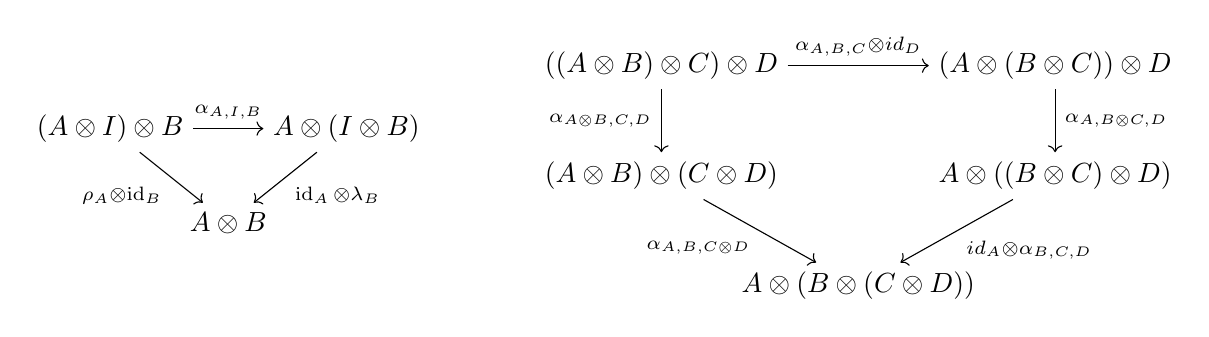
\begin{tikzpicture}[baseline=(current bounding box.center)]\label{cat:def:monoidalCat:pentagon}
  \node (AIB)  at (0,1.2)   {$(A \otimes I) \otimes B$};
  \node (AIB2) at (3,1.2)   {$A \otimes (I \otimes B)$};
  \node (AB)   at (1.5,0)     {$A \otimes B$};

  \draw[->] (AIB)  -- node[above] {$\scriptstyle \alpha_{A,I,B}$} (AIB2);
  \draw[->] (AIB)  -- node[below left]  {$\scriptstyle \rho_A \otimes \id_B$} (AB);
  \draw[->] (AIB2) -- node[below right] {$\scriptstyle \id_A \otimes \lambda_B$} (AB);
\begin{scope}[shift={(7.0,0)}]
  \node (TL) at (0,2)     {$((A \otimes B) \otimes C) \otimes D$};
  \node (TR) at (5,2)     {$(A \otimes (B \otimes C)) \otimes D$};
  \node (ML) at (0,0.6)   {$(A \otimes B) \otimes (C \otimes D)$};
  \node (MR) at (5,0.6)   {$A \otimes ((B \otimes C) \otimes D)$};
  \node (B)  at (2.5,-0.8)  {$A \otimes (B \otimes (C \otimes D))$};

  \draw[->] (TL) -- node[above] {$\scriptstyle \alpha_{A,B,C} \otimes id_D$} (TR);
  \draw[->] (TL) -- node[left]  {$\scriptstyle \alpha_{A \otimes B, C, D}$} (ML);
  \draw[->] (TR) -- node[right] {$\scriptstyle \alpha_{A, B \otimes C, D}$} (MR);
  \draw[->] (ML) -- node[below left]  {$\scriptstyle \alpha_{A,B,C \otimes D}$} (B);
  \draw[->] (MR) -- node[below right] {$\scriptstyle id_A \otimes \alpha_{B,C,D}$} (B);
\end{scope}
\end{tikzpicture}
\end{center}
For simplicity we denote a monoidal category as the sextuple $(\CC, \otimes, I, \alpha, \lambda, \rho   )$.
\end{definition}

Note that because we defined $- \otimes - : \CC \times \CC \to \CC$ to be a \emph{(bi)functor}, we immedeately gain the follwing relations by functoriality:
\begin{equation}\label{cat:monoidal:bifunctor}
  (f \ot g) \circ (f^\prime \ot g^\prime) = (f \circ f^\prime) \ot (g \circ g^\prime)
\end{equation}
\[
  \id_{A \otimes B} = \id_A \otimes \id_B 
\]

\begin{graphicalCalculus}
  We denote the elemenets of this Category by simple lines, and the morphisms as
  boxes between these lines. Since the tensor product corresponds to paralell
  execution, we describe tensored objects as parallel lines and tensored
  operators as parallel squares.
  \[
  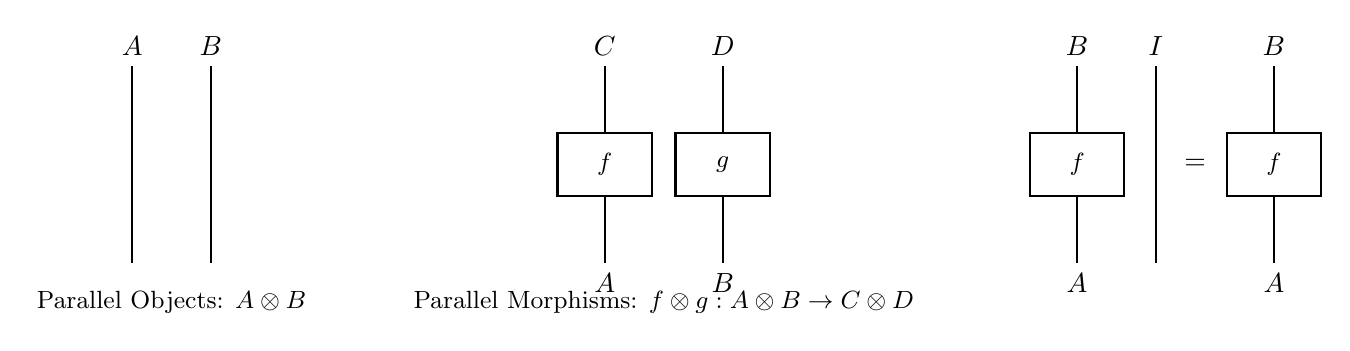
\begin{tikzpicture}[
    node distance=1.5cm and 1cm,
    thick,
    morphism/.style={draw, rectangle, minimum width=1.2cm, minimum height=0.8cm, fill=white, font=\small}
  ] 
    \begin{scope}
      % Strings / Objects
      \draw[thick] (0, 0) -- (0, 2.5) node[above] {$A$};
      \draw[thick] (1, 0) -- (1, 2.5) node[above] {$B$};
      
      \node at (0.5, -0.5) {\small Parallel Objects: $A \otimes B$};
    \end{scope}

    \begin{scope}[shift={(6,0)}]
      \node[morphism] (f) at (0, 1.25) {$f$};
      \node[morphism] (g) at (1.5, 1.25) {$g$};

      \draw[thick] (0, 0) node[below] {$A$} -- (f.south);
      \draw[thick] (1.5, 0) node[below] {$B$} -- (g.south);

      \draw[thick] (f.north) -- (0, 2.5) node[above] {$C$};
      \draw[thick] (g.north) -- (1.5, 2.5) node[above] {$D$};

      \node at (0.75, -0.5) {\small Parallel Morphisms: $f \otimes g : A \otimes  B \to C \otimes D$};
    \end{scope}

    \begin{scope}[shift={(12,0)}]
      \node[morphism] (f) at (0, 1.25) {$f$};

      \draw[thick] (0, 0) node[below] {$A$} -- (f.south);
      \draw[thick] (f.north) -- (0, 2.5) node[above] {$B$};
      
      \draw[thick] (1, 0) -- (1, 2.5) node[above] {$I$};

      \node at (1.5, 1.25) {$=$};

      \node[morphism] (f) at (2.5, 1.25) {$f$};

      \draw[thick] (2.5, 0) node[below] {$A$} -- (f.south);
      \draw[thick] (f.north) -- (2.5, 2.5) node[above] {$B$};

    \end{scope}
  \end{tikzpicture}
  \]
\end{graphicalCalculus}

The commuting condition in \cref{cat:def:monoidalCat:pentagon} is an instance of
the \emph{MacLane-coherence-theorem} \cite{maclane?} (for monoidal categories).
This essentially assert that no matter how many objects we look at, their
tensoring are isomorphic to each other without specifying another isomorphism on
higher spaces, but instead reusing the $\alpha$ associtator on $3$ strands is
enough.

\begin{example}
  Some examples of this tensor product here:
  \begin{enumerate}
    \item In $\Veck$, we denote the tensor product as $\ot_k$, and this is the
    default kronecker-product on $k$-vector spaces. The monoidal unit in this
    case is the field $k$. \todo{Does $k$ need to be algebraically closed?}
    \item The category $\Rep(G)$ is monoidal and has a tensor product by
    \cref{symm:def:tensor_product_representation}:
      \[
        (V \otimes_k W, \rho_{V \otimes_k W})
      \]
      and on morphisms $f \in \Hom_G(V_1, V_2), g \in \Hom_G(W_1,W_2)$ this
      gives 
      \[
        (f \otimes g)(v \otimes w) = f(v) \otimes g(w) \in \Hom_G(V_1 \ot_k W_1, V_2 \ot_k W_2)
      \]
    \item Take for example the $\Fib$ anyon theory. We can take products of
    anyons $a \otimes b$ and we can also identify the vacuum type $I$ over $a
    \otimes I = a$ and so on. \todo{rephrase!} However we also know that these
    anyons come in pairs, so they ought to be in a fusion channel. For now we do
    not have a concept of antiparticles or of fusion channels. We can only give
    the pairings of the anyons by bracketings of the monoidal tensors.
  \end{enumerate}
\end{example}

\begin{definition}
  Let $(\CC, \ot_\CC, 1_\CC)$ and $(D,\ot_D, 1_D)$ be monoidal categories. A \emph{\green{monoidal functor}} is a functor $F : \CC \to D$ that preserves the monoidal structure 
\end{definition}

\begin{definition}
Let $(\mathcal{V}, \ot_\mathcal{V}, I, \alpha, \lambda, \rho)$ be a monoidal category. A category
$\CC$ \green{\emph{enriched over $\mathcal{V}$}} (or a \emph{$\mathcal{V}$-category})
consists of
\begin{enumerate}
  \item for every $A, B \in \ob(\CC)$, a \emph{hom-object} $\Hom_\CC(A,B) \in \mathcal{V}$ (as opposed to Set in normal category),
  \item for every triple $A,B,C \in \ob(\CC)$, a \emph{composition morphism} in $\mathcal{V}$
  \[
    \circ_{A,B,C} : \Hom_\CC(B,C) \ot_\mathcal{V} \Hom_\CC(A,B) \longrightarrow \Hom_\CC(A,C),
  \]
  \item for every $A \in \ob(\CC)$, a \emph{unit morphism} in $\mathcal{V}$
  \[
    j_A : I \longrightarrow \Hom_\CC(A,A),
  \]
\end{enumerate}
\end{definition}

This immedeately gives us another defintion: 
\[
  \Hom_\CC(-,X) : \CC \to \mathcal{V} \quad \text{ is a contravariant functor. }
\]


\begin{definition}[\cite{joyalGeometryTensorCalculus1991}]\label{cat:def:braidedMonoidalCat}
A \emph{\green{braided monoidal category}} is a monoidal category $(\mathcal{C},
\otimes, I, \alpha, \lambda, \rho)$ equipped with an additional isomorphism, the
\emph{\green{braiding}}
\[
  \beta_{A,B} : A \otimes B \; \cong \; B \otimes A,
\]
on $A$ and $B$ satisfying
\begin{equation}\label{cat:braiding_naturality}
  \beta_{A,B\otimes C} = (\id_A \otimes \beta_{A,C}) \circ (\beta_{A,B} \otimes \id_C) \quad\text{ and }\quad \beta_{A \otimes B, C} = (\beta_{A,C} \otimes \id_B) \circ (\id_A \otimes \beta_{B,C}).
\end{equation} 

As a consequence, the \emph{hexagon} relations commute for all $A,B,C \in
\mathcal{C}$:

\begin{center}
% https://q.uiver.app/#q=WzAsMTIsWzAsMCwiKEEgXFxvdGltZXMgQikgXFxvdGltZXMgQyJdLFsxLDAsIkEgXFxvdGltZXMoQlxcb3RpbWVzIEMpIl0sWzIsMCwiKEIgXFxvdGltZXMgQylcXG90aW1lcyBBIl0sWzAsMSwiKEJcXG90aW1lcyBBKVxcb3RpbWVzIEMiXSxbMSwxLCJCIFxcb3RpbWVzIChBIFxcb3RpbWVzIEMpIl0sWzIsMSwiQiBcXG90aW1lcyAoQyBcXG90aW1lcyBBKSJdLFszLDAsIkEgXFxvdGltZXMgKEIgXFxvdGltZXMgQykiXSxbNCwwLCIoQSBcXG90aW1lcyBCKSBcXG90aW1lcyBDIl0sWzUsMCwiQ1xcb3RpbWVzKEFcXG90aW1lcyBCKSJdLFszLDEsIkEgXFxvdGltZXMoQyBcXG90aW1lcyBCKSJdLFs0LDEsIihBIFxcb3RpbWVzIEMpXFxvdGltZXMgQiJdLFs1LDEsIihDIFxcb3RpbWVzIEEpIFxcb3RpbWVzIEIiXSxbMCwxLCJcXGFscGhhIl0sWzEsMiwiXFxiZXRhX3tBLEJcXG90aW1lcyBDfSJdLFszLDQsIlxcYWxwaGEiXSxbNCw1LCJcXGlkX0IgXFxvdGltZXNcXGJldGFfe0EsQ30iXSxbMCwzLCJcXGJldGFfe0EsQn1cXG90aW1lcyBcXGlkX0MiLDJdLFsyLDUsIlxcYWxwaGEiXSxbNiw3LCJcXGFscGhhXnstMX0iXSxbNiw5LCJcXGJldGEiLDJdLFs5LDEwLCJcXGFscGhhXnstMX0iLDJdLFs3LDgsIlxcYmV0YSJdLFs4LDExLCJcXGFscGhhXnstMX0iXSxbMTAsMTEsIlxcYmV0YSIsMl1d
\begin{tikzcd}[column sep=scriptsize]
	{(A \otimes B) \otimes C} & {A \otimes(B\otimes C)} & {(B \otimes C)\otimes A} & {A \otimes (B \otimes C)} & {(A \otimes B) \otimes C} & {C\otimes(A\otimes B)} \\
	{(B\otimes A)\otimes C} & {B \otimes (A \otimes C)} & {B \otimes (C \otimes A)} & {A \otimes(C \otimes B)} & {(A \otimes C)\otimes B} & {(C \otimes A) \otimes B}
	\arrow["\alpha", from=1-1, to=1-2]
	\arrow["{\beta_{A,B}\otimes \id_C}"', from=1-1, to=2-1]
	\arrow["{\beta_{A,B\otimes C}}", from=1-2, to=1-3]
	\arrow["\alpha", from=1-3, to=2-3]
	\arrow["{\alpha^{-1}}", from=1-4, to=1-5]
	\arrow["\beta"', from=1-4, to=2-4]
	\arrow["\beta", from=1-5, to=1-6]
	\arrow["{\alpha^{-1}}", from=1-6, to=2-6]
	\arrow["\alpha", from=2-1, to=2-2]
	\arrow["{\id_B \otimes\beta_{A,C}}", from=2-2, to=2-3]
	\arrow["{\alpha^{-1}}"', from=2-4, to=2-5]
	\arrow["\beta"', from=2-5, to=2-6]
\end{tikzcd}
\end{center}
\end{definition}

\begin{definition}
A braided monoidal category is \emph{\green{symmetric}} if $\beta_{B,A} \circ
\beta_{A,B} = \mathrm{id}_{A \otimes B}$ for all $A, B$.
\end{definition}

\begin{lemma}
  The \emph{Yang-Baxter equation}\todo{define this somewhere} holds for the braiding:
  \[
    (\beta_{A,B} \ot \id_textC)(\id_A \ot \beta_{A,C})(\beta_{B,C} \ot \id_A) = 
  \]
\end{lemma}

\begin{graphicalCalculus}
  Now the graphical calculus changes, as we need to consider whether the
  braidings defined by $\beta$ are over or under. We denote the simple braidings
  as \todo{Check for the correct definition of the ambient space here.}
  \[
    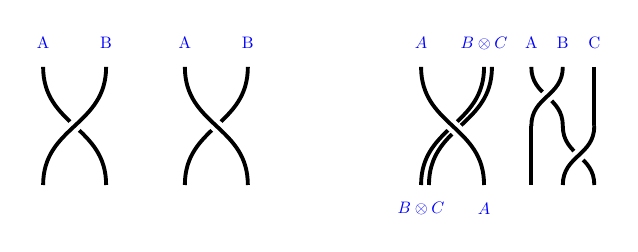
\begin{tikzpicture}[yscale=1.0]
      \draw (-0.40, 0.3) node {\color{blue}\scalebox{.6}{A}};
      \draw (0.40, 0.3) node {\color{blue}\scalebox{.6}{B}};
      \draw[line width=1.4] (-0.40, 0.00) .. controls (-0.40, -0.75) and (0.40, -0.75) .. (0.40, -1.50);
      \draw[line width=4.5, white] (0.40, 0.00) .. controls (0.40, -0.75) and (-0.40, -0.75) .. (-0.40, -1.50);
      \draw[line width=1.4] (0.40, 0.00) .. controls (0.40, -0.75) and (-0.40, -0.75) .. (-0.40, -1.50);
    
      \begin{scope}[shift={(1,0)}]
        \draw (0.40, 0.3) node {\color{blue}\scalebox{.6}{A}};
        \draw (1.20, 0.3) node {\color{blue}\scalebox{.6}{B}};
        \draw[line width=1.4] (1.20, 0.00) .. controls (1.20, -0.75) and (0.40, -0.75) .. (0.40, -1.50);
        \draw[line width=4.5, white] (0.40, 0.00) .. controls (0.40, -0.75) and (1.20, -0.75) .. (1.20, -1.50);
        \draw[line width=1.4] (0.40, 0.00) .. controls (0.40, -0.75) and (1.20, -0.75) .. (1.20, -1.50);
      \end{scope}

      \begin{scope}[shift={(4,0)}]
  \draw (0.40, 0.3) node {\color{blue}\scalebox{.6}{$A$}};
  \draw (1.20, 0.3) node {\color{blue}\scalebox{.6}{$B \ot C$}};
  \draw[line width=1.4] (1.20, 0.00) .. controls (1.20, -0.75) and (0.40, -0.75) .. (0.40, -1.50);
  \draw[line width=1.4] (1.30, 0.00) .. controls (1.30, -0.75) and (0.50, -0.75) .. (0.50, -1.50);
  \draw[line width=4.5, white] (0.40, 0.00) .. controls (0.40, -0.75) and (1.20, -0.75) .. (1.20, -1.50);
  \draw[line width=1.4] (0.40, 0.00) .. controls (0.40, -0.75) and (1.20, -0.75) .. (1.20, -1.50);
  \draw (1.20, -1.80) node {\color{blue}\scalebox{.6}{$A$}};
  \draw (0.40, -1.80) node {\color{blue}\scalebox{.6}{$B \ot C$}};
  \end{scope}

  \begin{scope}[shift={(6,0)}, scale=0.5]
  \draw (-0.40, 0.6) node {\color{blue}\scalebox{.6}{A}};
  \draw ( 0.40, 0.6) node {\color{blue}\scalebox{.6}{B}};
  \draw ( 1.20, 0.6) node {\color{blue}\scalebox{.6}{C}};
  \draw[line width=1.4] (1.20, 0.00) to (1.20, -1.50);

  \draw[line width=1.4] (-0.40, 0.00) .. controls (-0.40, -0.75) and (0.40, -0.75) .. (0.40, -1.50);
  \draw[line width=4.5, white] (0.40, 0.00) .. controls (0.40, -0.75) and (-0.40, -0.75) .. (-0.40, -1.50);
  \draw[line width=1.4] (0.40, 0.00) .. controls (0.40, -0.75) and (-0.40, -0.75) .. (-0.40, -1.50);

  \draw[line width=1.4] (-0.40, -1.50) to (-0.40, -3.00);
  \draw[line width=1.4] (0.40, -1.50) .. controls (0.40, -2.25) and (1.20, -2.25) .. (1.20, -3.00);
  \draw[line width=4.5, white] (1.20, -1.50) .. controls (1.20, -2.25) and (0.40, -2.25) .. (0.40, -3.00);
  \draw[line width=1.4] (1.20, -1.50) .. controls (1.20, -2.25) and (0.40, -2.25) .. (0.40, -3.00);
  \end{scope}
\end{tikzpicture}
  \]
\end{graphicalCalculus}

\begin{example}
  \begin{enumerate}
    \item In $\Veck$ this mapping is trivial.
    \item For representations, there exist transformations on the basis states,
    for example the theory $\Rep(\SU{2})$ picks up the phase $(-1)^{j_a + j_b +
    j_c}$\todo{Notation!}. For all categories built from representations of
    groups, these are symmetric.
    \item For anyons, these correspond to the phase picked up when exchaning the
    anyons. For abelian anyons, these braidings are symmetric indeed, however
    for nonabelians these create non-symmetric categories.
  \end{enumerate}
\end{example}


If we want to use contractions between matchings legs, and overall want the
ability to take duals just like in $\FDVec{\C}$, we need both a concept of
duality and the evaluation maps. This is also the categorification of the
\emph{creation} and \emph{annihilation} maps from \Cref{sect:Anyons}. Let this
motivate the following definition:
\begin{definition}
  A monoidal category $(\CC, \otimes, 1)$ is \emph{\green{rigid}} if, for every $A \in \CC$, there exists a \emph{\green{dual object}} $A^\ast$ with the following maps:
  \[
    \ev_A : A^\ast \otimes A \to 1 \quad \text{ and } \quad \coev_A : 1 \to A \otimes A^\ast
  \]
  subject to the diagrammatic constraints
% MODIFIED
% https://q.uiver.app/#q=WzAsMTIsWzAsMCwiQSJdLFsyLDAsIjFcXG90IEEiXSxbNCwwLCIoQSBcXG90IEFeXFxhc3QpIFxcb3QgQSJdLFs2LDAsIkFcXG90KEFeXFxhc3QgXFxvdCBBKSJdLFs4LDAsIkEgXFxvdCAxICJdLFsxMCwwLCJBIl0sWzAsMiwiQV5cXGFzdCJdLFsyLDIsIiBBXlxcYXN0IFxcb3QgMSJdLFs0LDIsIkFeXFxhc3QgXFxvdCAoQSBcXG90IEFeXFxhc3QpIl0sWzYsMiwiKEFeXFxhc3QgXFxvdCBBKSBcXG90IEFeXFxhc3QiXSxbOCwyLCIxIFxcb3QgQV5cXGFzdCJdLFsxMCwyLCJBXlxcYXN0Il0sWzQsNSwiXFxyaG9fQSJdLFszLDQsIlxcaWRfQSBcXG90IFxcZXZfQSJdLFsyLDMsIlxcYWxwaGFfe0EsQV5cXGFzdCxBfSJdLFsxLDIsIlxcY29ldl9BIFxcb3QgXFxpZF9BIl0sWzAsMSwiXFxsYW1iZGFfQSJdLFs3LDgsIlxcaWRfe0FeXFxhc3R9IFxcb3QgXFxjb2V2X3tBfSJdLFs4LDksIlxcYWxwaGFfe0FeXFxhc3QsQSxBXlxcYXN0fSJdLFs5LDEwLCJcXGV2X0EgXFxvdCBcXGlkX3tBXlxcYXN0fSJdLFsxMCwxMSwiXFxsYW1iZGFfe0FeXFxhc3R9Il0sWzYsNywiXFxyaG9fe0FeXFxhc3R9Il1d
\[\begin{tikzcd}[cramped, column sep=scriptsize]
	A && {1\ot A} && {(A \ot A^\ast) \ot A} && {A\ot(A^\ast \ot A)} && {A \ot 1 } && A \\
	\\
	{A^\ast} && { A^\ast \ot 1} && {A^\ast \ot (A \ot A^\ast)} && {(A^\ast \ot A) \ot A^\ast} && {1 \ot A^\ast} && {A^\ast}
	\arrow["{\lambda_A}", from=1-1, to=1-3]
	\arrow["{\coev_A \ot \id_A}", from=1-3, to=1-5]
	\arrow["{\alpha_{A,A^\ast,A}}", from=1-5, to=1-7]
	\arrow["{\id_A \ot \ev_A}", from=1-7, to=1-9]
	\arrow["{\rho_A}", from=1-9, to=1-11]
  \arrow[from=1-1, to=1-11, u path, "\id_A"' {below, distance=2pt}]
	\arrow["{\rho_{A^\ast}}", from=3-1, to=3-3]
	\arrow["{\id_{A^\ast} \ot \coev_{A}}", from=3-3, to=3-5]
	\arrow["{\alpha_{A^\ast,A,A^\ast}}", from=3-5, to=3-7]
	\arrow["{\ev_A \ot \id_{A^\ast}}", from=3-7, to=3-9]
	\arrow["{\lambda_{A^\ast}}", from=3-9, to=3-11]
  \arrow[from=3-1, to=3-11, u path, "\id_{A^\ast}"' {below, distance=2pt}]
\end{tikzcd}\]
  % https://q.uiver.app/#q=WzAsOCxbMCwwLCIxIFxcb3RpbWVzIEEiXSxbMiwwLCIoQSBcXG90aW1lcyBBXlxcYXN0KSBcXG90aW1lcyBBIl0sWzAsMiwiQSBcXG90aW1lcyAxIl0sWzIsMiwiQSBcXG90aW1lcyAoQV5cXGFzdCBcXG90aW1lcyBBKSJdLFs0LDIsIjEgXFxvdGltZXMgQV5cXGFzdCJdLFs0LDAsIkFeXFxhc3RcXG90aW1lcyAxIl0sWzYsMiwiKEFeXFxhc3QgXFxvdGltZXMgQSkgXFxvdGltZXMgQV5cXGFzdCJdLFs2LDAsIkFeXFxhc3QgXFxvdGltZXMgKEEgXFxvdGltZXMgQV5cXGFzdCkiXSxbMCwxLCJcXGNvZXZfQSBcXG90aW1lcyBcXGlkX0EiXSxbMCwyLCJcXGxhbWJkYV9BIFxcY2lyYyBcXHJob19BIiwyXSxbMiwzLCJcXGlkXzEgXFxvdGltZXMgXFxldl9BIiwyXSxbMSwzLCJcXGFscGhhX3tBLEFeXFxhc3QsQX0iXSxbNCw2LCJcXGV2X0EgXFxvdGltZXNfe0FeXFxhc3R9IiwyXSxbNSw0LCJcXGxhbWJkYV97QV5cXGFzdH0gXFxjaXJjIFxccmhvX3tBXlxcYXN0fSIsMl0sWzYsNywiXFxhbHBoYV97QV5cXGFzdCxBLEFeXFxhc3R9IiwyXSxbNSw3LCJcXGlkX0EgXFxvdGltZXMgXFxjb2V2X0EiXV0=
  %\[\begin{tikzcd}
	%  {1 \otimes A} && {(A \otimes A^\ast) \otimes A} && {A^\ast\otimes 1} && {A^\ast \otimes (A \otimes A^\ast)} \\
	%  \\
	%  {A \otimes 1} && {A \otimes (A^\ast \otimes A)} && {1 \otimes A^\ast} && {(A^\ast \otimes A) \otimes A^\ast}
	%  \arrow["{\coev_A \otimes \id_A}", from=1-1, to=1-3]
	%  \arrow["{\lambda_A \circ \rho_A}"', from=1-1, to=3-1]
	%  \arrow["{\alpha_{A,A^\ast,A}}", from=1-3, to=3-3]
	%  \arrow["{\id_A \otimes \coev_A}", from=1-5, to=1-7]
	%  \arrow["{\lambda_{A^\ast} \circ \rho_{A^\ast}}"', from=1-5, to=3-5]
	%  \arrow["{\id_1 \otimes \ev_A}"', from=3-1, to=3-3]
	%  \arrow["{\ev_A \otimes_{A^\ast}}"', from=3-5, to=3-7]
	%  \arrow["{\alpha_{A^\ast,A,A^\ast}}"', from=3-7, to=1-7]
  %\end{tikzcd}\]
\end{definition}

\begin{example}
  \begin{enumerate}
    \item 
  In $\Veck$, the dual object for every vector space $V$ is given by its \emph{dual-space} $V^\ast \coloneqq \Hom(V, k)$. The evaluation and coevaluation maps here correspond to 
  \[
    \ev_V : V \otimes V^\ast \to k, 
  \]
  \[
    \coev_V : k \to V^\ast \otimes V, 
  \]
    \item 
    In Anyon theories we generally want the ability to take antiparticles for
    each species of anyon, and furthermore, we want to be able to \emph{create}
    and \emph{annihilate} these anyons. So the dual object corresponds to the
    antiparticle, and the $\ev$ and $\coev$ maps either produce a
    particle-antiparticle pair from the vacuum or annihilate them (to a state
    containing the vacuum).
  \end{enumerate}
\end{example}

\newcommand{\Astrand}[2]{
  \draw[->, #1] (#2) -- ++(0,1);
}
\newcommand{\Adualstrand}[2]{
  \draw[<- , #1] (#2) -- ++(0,1);
}

\begin{graphicalCalculus}
  \todo{Do these need to point up or down?} Now we have to introduce this notion
  of duality on the level of the graphical calculus. We denote an object in the
  category by an oriented arrow, and denote its dual object by the reverse.
  \[
    \begin{tikzpicture}[baseline=-0.5ex]
      \Astrand{}{0,0}
      \node[right] at (0.1,0.5) {$A$};
    \end{tikzpicture}
    \qquad\qquad
    \begin{tikzpicture}[baseline=-0.5ex]
      \Adualstrand{}{0,0}
      \node[right] at (0.1,0.5) {$A^\ast$};
    \end{tikzpicture}
  \]
  Similarly the $\ev_{A}$ and $\coev_A$ maps induce a graphical menaing:
  \[
  \coev_A :
  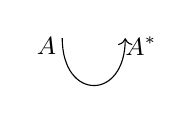
\begin{tikzpicture}[baseline=-0.5ex]
    \draw[->] (-0.4, 0.6) .. controls (-0.4, -0.2) and (0.4, -0.2) .. (0.4, 0.6);
    \node at (-0.6, 0.5) {\small $A$};
    \node at (0.6, 0.5) {\small $A^*$};
  \end{tikzpicture}
  \qquad\text{and}\qquad
  \ev_A :
  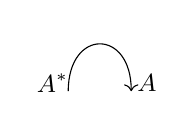
\begin{tikzpicture}
    \draw[->] (-0.4, -0.6) .. controls (-0.4, 0.2) and (0.4, 0.2) .. (0.4, -0.6);
    \node at (-0.6, -0.5) {\small $A^*$};
    \node at (0.6, -0.5) {\small $A$};
  \end{tikzpicture}.
\]

\end{graphicalCalculus}

Observe that in the graphical calculus, we denoted this as a bent arrow from $A \to A^\ast$. In fact, we gain the following identities:
\[
  \Hom_\CC(X \ot A, Y) \cong \Hom_\CC(X, A^\ast \ot Y) : f \mapsto 
\]
We can also build dualities for morphisms here: Let $f : A \to B$ be arbitrary and define
\[
  f^\ast : B^\ast \to A^\ast = (\ev_B \ot \id_{A^\ast})(\id_{B^\ast} \ot f \ot \id_{A^\ast})(\id_{B^\ast} \ot \coev_A)
\]
This gives us a few additional theorems:
\begin{enumerate}
  \item $\id^\ast_A = \id_{A^\ast}$
  \item $(g \circ f)^\ast = f^\ast \circ g^\ast$ 
  \item $(f \ot g)^\ast = g^\ast \ot f^\ast$
  \item $f \mapsto f^\ast$ is linear
\end{enumerate}
Also notice by this that $(-)^\ast$ is a contravariant functor.

Further the natural observation that $A \cong A^{\ast\ast}$ holds should be
encoded in these categories.
\begin{definition}
  A \emph{\green{pivotal structure}} on a rigid monoidal category is given by a natural isomorphism $\id \to (-)^{\ast\ast}$, i.e. a collection of isomorphisms that identify $\{A \to A^{\ast\ast}\}$.
\end{definition}

This allows us to define a notion of a traced category.
\begin{definition}
  We can define a notion of a \emph{\green{right trace}} on any endomorphism $V
  \to V$ in such categories:
    % https://q.uiver.app/#q=WzAsNSxbMSwwLCIxIl0sWzMsMCwiQSBcXG90aW1lcyBBXlxcYXN0Il0sWzUsMCwiQV57XFxhc3RcXGFzdH0gXFxvdCBBXlxcYXN0Il0sWzcsMCwiMSJdLFswLDAsIlxcdHJfUiJdLFswLDEsIlxcY29ldl9BIl0sWzEsMiwiKFxcZGVsdGFfQSBcXGNpcmMgKC0pIFxcb3QgXFxpZF97QV5cXGFzdH0pIl0sWzIsMywiXFxldl97QV5cXGFzdH0iXSxbNCwwLCJcXGNvbG9uZ2VxcSIsMSx7InN0eWxlIjp7ImJvZHkiOnsibmFtZSI6Im5vbmUifSwiaGVhZCI6eyJuYW1lIjoibm9uZSJ9fX1dXQ==
  \[\begin{tikzcd}[cramped]\label{cat:eq:Rtrace}
	  {\tr_R} & 1 && {A \otimes A^\ast} && {A^{\ast\ast} \ot A^\ast} && 1
	  \arrow["\coloneqq"{description}, draw=none, from=1-1, to=1-2]
	  \arrow["{\coev_A}", from=1-2, to=1-4]
	  \arrow["{(\delta_A \circ (-)) \ot \id_{A^\ast}}", from=1-4, to=1-6]
	  \arrow["{\ev_{A^\ast}}", from=1-6, to=1-8]
    \end{tikzcd}\]
\end{definition}

\begin{definition}
  A pivotal rigid braided monoidal category is called \emph{\green{spherical}}
  if 
  \[
    \tr_R = \tr_L
  \]
  and we can further define the \emph{\green{quantum dimension}} of an object
  $A$ as
  \begin{equation}\label{cat:eq:dim}
    \dim(A) = \tr(\id_A)
  \end{equation}
\end{definition}

\begin{graphicalCalculus}
  The usage of \emph{spherical} here derives from the fact that we can
  arbitrarily reorder our string calculus on the surface of the $2$-sphere:
  \todo{Does this lead naturally into the ribbon being the only obstacle to
  planarity?}Consider for example the trace where the connecting strand is
  swapped around the back of the sphere.
  \begin{figure}[H]
    \centering
    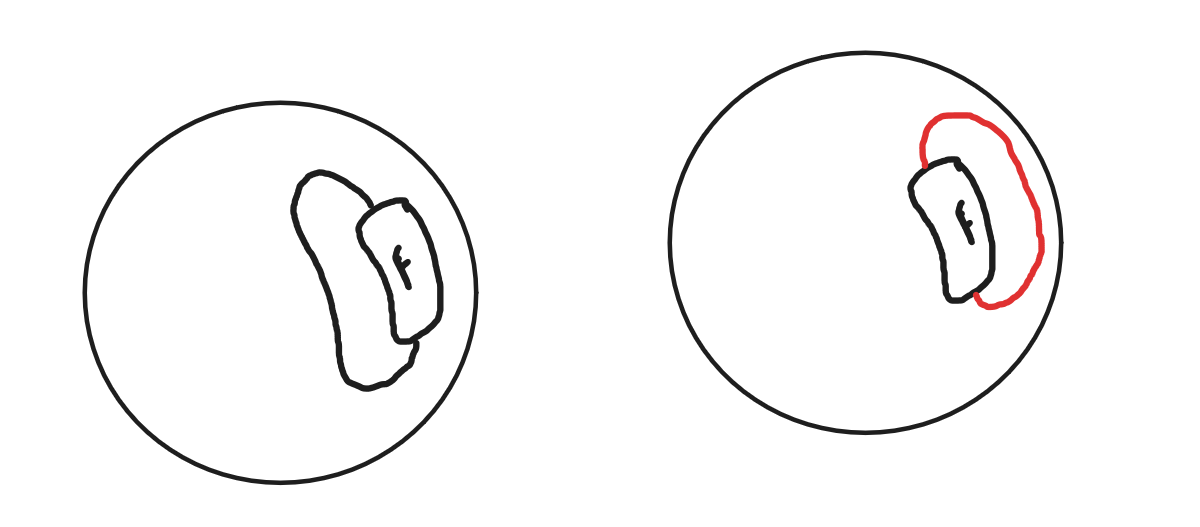
\includegraphics[width=0.8\textwidth]{figures/sphericalcat.png}
  \end{figure}
\end{graphicalCalculus}

\begin{lemma}
  State without proof, in any spherical category $\CC$ we can make the following
  statements about the trace. Let $A\in\CC$ and $f,g\in\End(A)$ arbitrary, let 
  \[
    \tr : \End_\CC(A) \to \End_\CC(\mathrm{I})
  \]
  \begin{enumerate}
    \item $\tr(f^\ast) = \tr(f)$
    \item $\tr(f \otimes g) = \tr(f) \cdot \tr(g)$
    \item $\tr(h \circ k) = \tr(k \circ h)$
    \item \todo{Likely more, but which ones do we actually need?}
  \end{enumerate}
\end{lemma}

So there is two reasons that we need this morphism here. One is to resolve the
third Reidemeister move (which we havent introduced yet!) and another is that we
can consider anyons to have an intrinsic rotation, however, this would
contradict that we considered them equivalent particles with no degrees of
freedom. I think \cite{burtonShortGuideAnyons2016} uses a deformed braid group
for this, but I would need to double check this.

\begin{definition}
  A \emph{\green{ribbon}} category is a braided monoidal rigid category
  $(\CC,\otimes,1,\alpha,\gamma,\rho,\beta,\ev,\coev)$ with maps $\theta_A : A
  \to A$ that realizes a \emph{self-braiding} of the object. This is subject to
  \[
    \theta_{A \otimes B} = (\theta_A \otimes \theta_B) \circ \beta_{B,A} \circ \beta_{A,B}
  \]
  as well as
  \[  
    \theta_{A^\ast} = (\theta_A)^\ast
  \]
\end{definition}

\begin{example}
  Since this is an endomorphism, physically this acts by a phase.
\end{example}


\begin{definition}\label{cat:def:directSum}
  Given a linear category $\CC$ with objects $\{A_j\}_{j=1}^N \subseteq \ob(\CC)$, an object $\bigoplus_{i=1}^n A_i \in \CC$ is
  called the \emph{\green{direct sum}} if it is equipped with the injection and projection
  map
  \[
    \iota_i : A_j \to \bigoplus A_i \quad \text{ and } \quad \pi_i : \bigoplus A_j \to A_i 
  \]
  such that
  \[
    \pi_i \circ \iota_i = \id_{A_i} \forall i \quad \text{ and } \quad \sum_{i}^{} \iota_i \pi_i = \id_{\bigoplus A_i}
  \]
\end{definition}

A great resource on semisimple categories \cite{bailieSemisimple2017}.

\begin{definition}\label{cat:def:semisimpleCategory} A \emph{\green{semisimple}}
  category\footnote{There are multiple definitions of semisimplicity and
  semisimple categories, and here we are using the definition of \emph{object
  simplicity}. A review of these definitions is given in
  \cite{bailieSemisimple2017}.} is a category in which every object $S \in
  \ob(\CC)$ decomposes as a finite direct sum 
  \begin{equation}\label{cat:eq:semisimple_decomp_1}
    S \cong \bop_i S_i, \qquad S_i \text{ simple }
  \end{equation}
  where a \emph{\green{simple}} object is an object, where for any other object
  $A$ that admits an injective \todo{this is vector space intuition, not sure if
  this works. Maybe we need to introduce monomorphism? Need to review this
  definition for general categories.} map, the object is either the $0$ morphism
  or an isomorphism to $S$ \todo{Is this just the first part of schurs lemma?}.
  If we group these simples by isomorphism, we can restate \eqref{cat:eq:semisimple_decomp_1} equivalently as
  $$
    S \cong \bop_i S_i^{\oplus n_i}
  $$
  where $n_i = \dim\Hom_\CC(S_i, S)$. Note that by our assumption of
  $\Veck$-enrichment, all the $n_i$s are finite. \todo{Erichment first.} Further
  denote the set of simple objects by $\Irr(\CC) \subseteq \ob(\CC)$.
\end{definition}

\begin{example}
  \begin{enumerate}
    \item In $\Rep(G)$, we know that either the representations are simple
      (Irreps) or they decompose as some direct sum representation.
    \item In Anyonic theories, we primarily only consider simple objects $a,b,c
      \ldots$ and tensor products between them. Then we assign each
      combinationof anyons a fusion outcome $a \otimes b = c \oplus d \oplus
      \cdots$. 
  \end{enumerate}
  
\end{example}

\begin{lemma}[Schur's lemma
    \cite{deutscheakademiederwissenschaftenzuberlinSitzungsberichteKoeniglichPreussischen1882}
  ]
  \label{cat:lemma:schur}
  If $A$ and $B$ are simple objects in a linear category over an algebraically
  closed field $k$ (this is always $\C$ in our case), then it holds that
  \[
    \Hom(A,B) = \begin{dcases}
      k \cdot \id_S, &\text{ if } A \cong B ;\\
      0 , &\text{ if } A \ncong B .
    \end{dcases}
  \]
  Proof \cite[Theorem~7.5]{ibortIntroductionGroupsGroupoids2019}.
\end{lemma}

Now assume that we take a semisimple category that is also monoidal. By
semisimplicity, any of the objects of the form $R_a \ot R_b$ are isomoprhic to $\bop R_c$
where $R_a,R_b, \{R_c\}$ are all simple. A simple consequence of \Cref{cat:lemma:schur} produces
\[
  \dim \Hom_\CC(R_a \ot R_b, R_c) 
  = \dim \Hom_\CC (\bop_c N^{ab}_d R_d, R_c) 
  = \dim \bop_d \Hom_\CC (R_d, R_c)^{\op N^{ab}_d} 
  \overeq{\cref{cat:lemma:schur}} \dim k^{N^{ab}_c}
\]
Call this isomorphism $\Phi: \bigoplus_{c,\mu} R_c \to R_a \otimes R_b$. Then we
can extend projection and injection maps in dependence of the tensor product by
the following diagram:
\begin{equation}\label{cat:eq:fusionprop}
% https://q.uiver.app/#q=WzAsNSxbMCwwLCJcXGJpZ29wbHVzX2MgUl9jIl0sWzIsMCwiUl9hIFxcb3RpbWVzIFJfYiJdLFswLDEsIlJfYyJdLFs0LDAsIlxcYmlnb3BsdXNfYyBSX2MiXSxbNCwxLCJSX2MiXSxbMCwxLCJcXFBoaSJdLFsyLDAsIlxcaW90YV9jIl0sWzIsMSwiXFxleGlzdHMgXFxpb3RhX3tjLFxcbXV9XnthYn0iLDJdLFsxLDMsIlxcUGhpXnstMX0iXSxbMyw0LCJcXHBpX2MiXSxbMSw0LCJcXGV4aXN0c1xccGlfe2FifV57YyxcXG11fSIsMl1d
%\begin{tikzcd}
%	{\bigoplus_c R_c} && {R_a \otimes R_b} && {\bigoplus_c R_c} \\
%	{R_c} &&&& {R_c}
%	\arrow["\Phi", from=1-1, to=1-3]
%	\arrow["{\Phi^{-1}}", from=1-3, to=1-5]
%	\arrow["{\exists\pi_{ab}^{c,\mu}}"', from=1-3, to=2-5]
%	\arrow["{\pi_c}", from=1-5, to=2-5]
%	\arrow["{\iota_c}", from=2-1, to=1-1]
%	\arrow["{\exists \iota_{c,\mu}^{ab}}"', from=2-1, to=1-3]
%\end{tikzcd}
% https://q.uiver.app/#q=WzAsNyxbMCwwLCJcXGJpZ29wbHVzX2MgUl9jIl0sWzMsMCwiUl9hIFxcb3RpbWVzIFJfYiJdLFswLDIsIlJfYyJdLFs2LDAsIlxcYmlnb3BsdXNfYyBSX2MiXSxbNiwyLCJSX2MiXSxbMSwwLCJcXGJpZ29wbHVzX3tcXG11LGN9Ul9jIl0sWzUsMCwiXFxiaWdvcGx1c197XFxtdSxjfVJfYyJdLFsyLDAsIlxcaW90YV9jIl0sWzIsMSwiXFxleGlzdHMgXFxpb3RhX3tjLFxcbXV9XnthYn0iLDJdLFszLDQsIlxccGlfYyJdLFsxLDQsIlxcZXhpc3RzXFxwaV97YWJ9XntjLFxcbXV9IiwyXSxbNSwxLCJcXFBoaSJdLFswLDUsIlxcaW90YV9cXG11Il0sWzIsNSwiXFxpb3RhX3tjLFxcbXV9IiwxXSxbMSw2LCJcXFBoaV57LTF9Il0sWzYsMywiXFxwaV9cXG11Il0sWzYsNCwiXFxwaV97XFxtdSxjfSIsMV1d
\begin{tikzcd}[cramped]
	{\bigoplus_c R_c} & {\bigoplus_{\mu,c}R_c} && {R_a \otimes R_b} && {\bigoplus_{\mu,c}R_c} & {\bigoplus_c R_c} \\
	\\
	{R_c} &&&&&& {R_c}
	\arrow["{\iota_\mu}", from=1-1, to=1-2]
	\arrow["\Phi", from=1-2, to=1-4]
	\arrow["{\Phi^{-1}}", from=1-4, to=1-6]
	\arrow["{\exists\pi_{ab}^{c,\mu}}"', from=1-4, to=3-7]
	\arrow["{\pi_\mu}", from=1-6, to=1-7]
	\arrow["{\pi_{\mu,c}}"{description}, from=1-6, to=3-7]
	\arrow["{\pi_c}", from=1-7, to=3-7]
	\arrow["{\iota_c}", from=3-1, to=1-1]
	\arrow["{\iota_{c,\mu}}"{description}, from=3-1, to=1-2]
	\arrow["{\exists \iota_{c,\mu}^{ab}}"', from=3-1, to=1-4]
\end{tikzcd}
\end{equation}

Furthermore, these admit similar constraints as the direct sum:
\begin{equation}
  \pi^{c,\mu}_{ab} \iota_{d,\nu}^{ab} = \pi_{c,\mu} \Phi^{-1}\Phi  \iota_{d,\nu} = \delta_{cd}\delta_{\mu\nu} \id_{R_c}
\end{equation}
and
\begin{equation}\label{cat:eq:basis_completeness}
  \sum_{c,\mu}^{} \iota_{c,\mu}^{ab} \pi^{c,\mu}_{ab} = \Phi \left(\sum_{c,\mu}^{} \iota_{c,\mu}\pi_{c,\mu}\right) \Phi^{-1} = \Phi \id_{\bigoplus R_{c}} \Phi^{-1} = \id_{R_a \otimes R_b}  
\end{equation}

We take these maps as above and claim they form a basis of the spaces $\Hom_\CC
(a \otimes b, c)$ and $\Hom_\CC (c, a \otimes b)$.

\begin{proof}
  First we show linear independence. Let $\{x_\mu\}_{1}^{N_c^{ab}}$ be a set of
  scalars and suppose that $\sum_\mu x_\mu \iota_{c,\mu}^{ab} = 0$. Observe that
  \[
    \pi_{c,\mu}^{ab} (\sum_{\mu} x_\mu \iota_{c,\mu}^{ab}) = \sum x_\mu \delta_{\mu,\nu} \id_{R_c} = x_\nu \id_{R_c}
  \]
  and since $\id_{R_c} \neq 0$ these form a linearly independent set. 

  Now let $f \in \Hom_\CC(R_c, R_a \ot R_b)$ be an arbitrary morphism. By
  \eqref{cat:eq:basis_completeness}, we can write
  \[
    f = \id_{R_a \ot R_b} \circ f = \sum_{d,\nu} \iota_{d,\nu}^{ab} (\pi^{d,\nu}_{ab} \circ f \in \Hom_\CC(R_c,R_d)) \overeq{\Cref{cat:lemma:schur}} \sum_{d,\nu} \iota_{d,\nu}^{ab} \delta_{R_c \cong R_d} \lambda_\nu \id_{R_c} = \sum_\nu \lambda_\nu \iota_{c,\nu}^{ab}
  \]
  and $f$ is an arbitrary linear combination and thus
  \[
    \text{span}_\C \left\{\iota_{d,\nu}^{ab}\right\}_{\nu = 1}^{N_{ab}^c} \cong \Hom_{\CC}(R_c, R_a \otimes R_b)
  \]
  and the statement follows dually for $\Hom_\CC(R_a \otimes R_b, R_c)$.
\end{proof}

%\begin{graphicalCalculus}
%  We carry over the graphical calculus for the monoidal categories (and all the
%  extra structure defined thus far) and introduce new notation for the nodes 
%\end{graphicalCalculus}

If we look at $\Hom$ spaces of a higher order such as $\Hom_\CC(R_d, (R_a \ot
R_b) \ot R_c)$, we have to choose a bracketing of the tensor products since we
can only associate $(R_a \ot R_b) \ot R_c \cong R_a \ot (R_b \ot R_c)$.
Under the (covariant) functor $\Hom_\CC(-, R_d)$ this introduces a pushforward
\[
  (\alpha_{abc}^d)^\ast : \Hom_\CC((R_a \ot R_b) \ot R_c, R_d) \cong \Hom_\CC(R_a \ot (R_b \ot R_c), R_d)
\]
and a pullback under $\Hom_\CC(R_d, -)$ 
\[
  (\alpha^{abc}_d)^\ast : \Hom_\CC(R_d, (R_a \otimes R_b \otimes R_c)) \cong \Hom_\CC(R_d, R_a \ot (R_b \ot R_c)).
\]
We can also define a basis for these extended spaces. In fact, lets generalize this to the space $\Hom_\CC(R_b, \bigotimes_{i=1}^n R_{a_i})$ where we assume this is fully left-algined bracketing. 

We define the higher bases recursively: Let $n > 2$ and intermediate labels
$e_1, e_2, \ldots, e_{n-2} \in \Irr(\CC)$ and multiplicity indices $\mu_1,
\ldots, \mu_{n-1}$. We fix some notation to let $\vec \mu_{k-1}$ to denote the
tuple of all labels up to $\mu_{k-1}$. Then we can define
\[
  \iota^{a_1 \cdots a_n}_{d,\hat e_{n-2},\hat\mu_{n-1}} \coloneqq \left(\iota^{a_1 \cdots a_{n-1}}_{e_{n-2},\vec e_{n-3},\vec\mu_{n-2}} \otimes \id_{R_{a_n}}\right) \circ \iota^{e_{n-2}a_n}_{d,\mu_{n-1}}.
\]
We can assume this holds by induction for $(n-1)$:
\[
  \pi^{a_1\cdots a_{n-1}}_{e;\vec e,\vec\mu}\circ
  \iota^{a_1\cdots a_{n-1}}_{e';\vec e\,',\vec\mu'}
  = \delta_{ee'}\,\delta_{\vec e\vec e\,'}\,\delta_{\vec\mu\vec\mu'}\;\id_{R_e}.
\]
\[
  \sum_{e,\vec e,\vec\mu}
  \iota^{a_1\cdots a_{n-1}}_{e;\vec e,\vec\mu}\circ
  \pi^{a_1\cdots a_{n-1}}_{e;\vec e,\vec\mu}
  = \id_{\bigotimes_{i<n}R_{a_i}}.
\]
\[
    \pi^{a_1\cdots a_n}_{c;\vec e,\vec\mu} \circ \iota^{a_1\cdots a_n}_{d;\vec f,\vec\nu}
    \overeq{\eqref{cat:monoidal:bifunctor}} \pi^{e_{n-2}a_n}_{c,\mu_{n-1}}\circ\Big[\big(\pi^{a_1\cdots a_{n-1}}_{e_{n-2};\vec e_{n-3},\vec\mu_{n-1}}
    \circ \iota^{a_1\cdots a_{n-1}}_{f_{n-2}; \vec f_{n-3}, \vec\nu_{n-1}}\big)\otimes\id_{R_{a_n}}\Big]
    \circ\iota^{f_{n-2}a_n}_{d,\nu_{n-1}}.
  \]
By the inductive hypothesis the bracket evaluates to
$\delta_{e_{n-2}f_{n-2}}\,\delta_{\vec e_{n-3}\vec f_{n-3}}\,
\delta_{\vec\mu_{n-2}\vec\nu_{n-2}}\,\id_{R_{e_{n-2}}}$,
and the $n=2$ case finishes orthoonality.

Let $e:=e_{n-2}$, $\iota'=\iota^{a_1\cdots a_{n-1}}_{e;\vec e_{n-3},\vec\mu_{n-2}}$,
and $\pi'$ likewise. Then
\[
  \sum_{d,\vec e,\vec\mu}
  \iota^{a_1\cdots a_n}_{d;\vec e,\vec\mu}\circ\pi^{a_1\cdots a_n}_{d;\vec e,\vec\mu}
  = \sum_{e,\vec e_{n-3},\vec\mu_{n-2}}
  (\iota'\ot\id_{R_{a_n}})\circ
  \Big[\sum_{d,\mu_{n-1}}
  \iota^{e a_n}_{d,\mu_{n-1}}\circ\pi^{e a_n}_{d,\mu_{n-1}}\Big]
  \circ(\pi'\ot\id_{R_{a_n}}).
\]

%\[
%  \pi^{a_1\cdots a_n}_{d;\vec e,\vec\mu}\circ\iota^{a_1\cdots a_n}_{d';\vec e\,',\vec\mu'}
%    = \pi^{e_{n-2}a_n}_{d,\mu_{n-1}}\circ\Big[\big(\pi^{a_1\cdots a_{n-1}}_{e_{n-2},\vec\mu_{n-1}}
%    \circ \iota^{a_1\cdots a_{n-1}}_{e'_{n-2},\vec\mu'_{n-1}}\big)\otimes\id_{R_{a_n}}\Big]
%    \circ\iota^{e'_{n-2}a_n}_{d',\mu'_{n-1}}.
%\]

In fact, we can also form a "canoncial" basis for the spaces $\Hom_\CC(X^{\ot
n}, X^{\ot n})$\todo{this needs a lot of conventions?} as given in
\cite{ValeraThesis}
\begin{equation}
\text{Hom}\left( \bigotimes_{k=1}^m X_{i_k}, \bigotimes_{l=1}^n X_{j_l} \right) = \text{span}_{\mathbb{C}} \left\{
\begin{gathered}
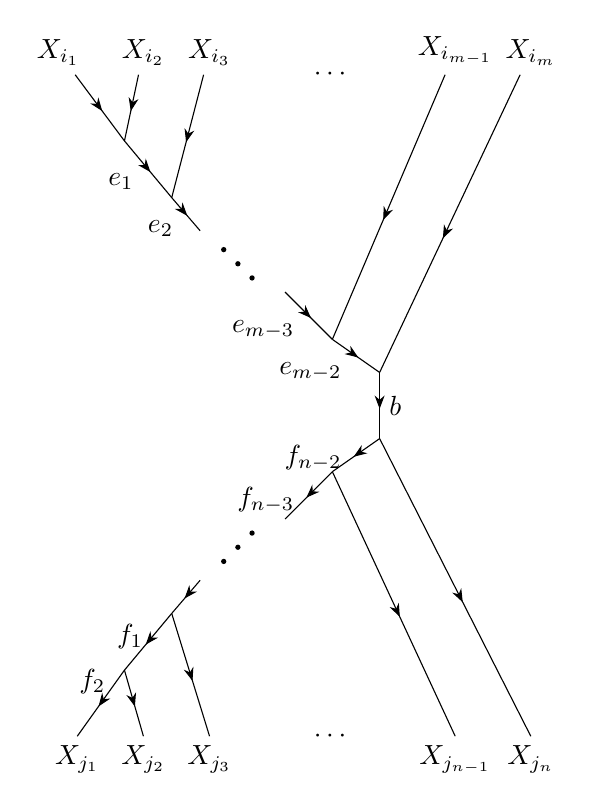
\begin{tikzpicture}[
    baseline=(current bounding box.center),
    scale=1.2,
    string arrow/.style={
        postaction={decorate},
        decoration={
            markings,
            mark=at position 0.55 with {\arrow[scale=1.0]{Stealth}}
        }
    }
]
    \node (xi1) at (-3.4, 3.2) [above] {$X_{i_1}$}; % I dont get why it is assym with -3.2
    \node (xi2) at (-2.5, 3.2) [above] {$X_{i_2}$};
    \node (xi3) at (-1.8, 3.2) [above] {$X_{i_3}$};
    \node at (-0.5, 3.2) {$\cdots$};
    \node (xim1) at (0.8, 3.2) [above] {$X_{i_{m-1}}$};
    \node (xim) at (1.6, 3.2) [above] {$X_{i_m}$};

    % Internal Vertices
    \coordinate (Ve1) at (-2.7, 2.5);
    \coordinate (Ve2) at (-2.2, 1.9);
    \coordinate (Vem3) at (-1.0, 0.9);
    \coordinate (Vem2) at (-0.5, 0.4);
    \coordinate (Btop) at (0, 0.05);

    \draw[string arrow] (xi1) -- (Ve1);
    \draw[string arrow] (xi2) -- (Ve1);
    \draw[string arrow] (xi3) -- (Ve2);
    \draw[string arrow] (xim1) -- (Vem2);
    \draw[string arrow] (xim) -- (Btop);

    \draw[string arrow] (Ve1) -- (Ve2) node[below left, pos=0.4] {$e_1$};
    \draw[string arrow] (Ve2) -- (-1.9, 1.55) node[below left, pos=0.4] {$e_2$};
    
    \fill (-1.65, 1.35) circle (0.8pt);
    \fill (-1.50, 1.20) circle (0.8pt);
    \fill (-1.35, 1.05) circle (0.8pt);
    
    %\draw[string arrow] (-1.2, 0.9) -- (Vem3); 
    \draw[string arrow] (Vem3) -- (Vem2) node[below left, pos=0.4] {$e_{m-3}$};
    \draw[string arrow] (Vem2) -- (Btop) node[below left, pos=0.4] {$e_{m-2}$};


    \coordinate (Bbot) at (0, -0.65);
    \draw[string arrow] (Btop) -- (Bbot) node[right, pos=0.5] {$b$};


    \coordinate (Vfn2) at (-0.5, -1.0);
    \coordinate (Vfn3) at (-1.0, -1.5);
    \coordinate (Vf2) at (-2.2, -2.5);
    \coordinate (Vf1) at (-2.7, -3.1);

    \draw[string arrow] (Bbot) -- (Vfn2) node[left, pos=0.6] {$f_{n-2}$};
    \draw[string arrow] (Vfn2) -- (Vfn3) node[left, pos=0.6] {$f_{n-3}$};
    
    \fill (-1.35, -1.65) circle (0.8pt);
    \fill (-1.50, -1.80) circle (0.8pt);
    \fill (-1.65, -1.95) circle (0.8pt);
    
    \draw[string arrow] (-1.9, -2.15) -- (Vf2);
    \draw[string arrow] (Vf2) -- (Vf1) node[left, pos=0.4] {$f_1$};
    \path (Vf2) -- (Vf1) node[left, pos=1.2] {$f_2$}; % Label position adjustment

    \draw[string arrow] (Vf1) -- (-3.2, -3.8);
    \draw[string arrow] (Vf1) -- (-2.5, -3.8);
    \draw[string arrow] (Vf2) -- (-1.8, -3.8);
    \draw[string arrow] (Vfn2) -- (0.8, -3.8);
    \draw[string arrow] (Bbot) -- (1.6, -3.8);

    \node (xj1) at (-3.2, -3.8) [below] {$X_{j_1}$};
    \node (xj2) at (-2.5, -3.8) [below] {$X_{j_2}$};
    \node (xj3) at (-1.8, -3.8) [below] {$X_{j_3}$};
    \node at (-0.5, -3.8) {$\cdots$};
    \node (xjn1) at (0.8, -3.8) [below] {$X_{j_{n-1}}$};
    \node (xjn) at (1.6, -3.8) [below] {$X_{j_n}$};

\end{tikzpicture}
\end{gathered}
\right\}_{ \substack{b, \, e_1, \dots,  e_{m-2}, \, f_1, \, \dots, \, f_{n-2} \\ \mu_1, \, \dots, \, \mu_{m-2}, \, \nu_1, \, \dots, \, \nu_{n-2}} }
\end{equation}

Now, what this construction allows us to do is as follows: Consider the decompositions
\begin{align*}
  \Hom_\CC((A \ot B) \ot C, D) &\cong \bop_{e \in \Irr(\CC)} \Hom_\CC(A \ot B, e) \ot_k \Hom_\CC(e \ot C, D) \\
  \Hom_\CC(A \ot (B \ot C)) &\cong \bop_{f \in \Irr(\CC)} \Hom_\CC(A \ot f, D) \ot_k \Hom_\CC(B \ot C, f)
\end{align*}
Which is induced by inverse of the isomorphism\todo{refer to basis}
\[
  \mu \ot_k \nu \mapsto (\mu \ot \id_c) \circ \nu.
\]

Using this we can coordinatize the pushforward as a matrix
\[
  F^{ABC}_D : \bop_{e \in \Irr(\CC)} \Hom_\CC(A \ot B, e) \ot_k \Hom_\CC(e \ot C, D) 
  \to \bop_{f \in \Irr(\CC)} \Hom_\CC(A \ot f, D) \ot_k \Hom_\CC(B \ot C, f)
\]
where the entries of this matrix are called the $6j$-symbols after Wigner.
However to actually get an element we need to specify 10
parameters\footnote{Wigner (on $\SU{2}$) considered theories that were
\emph{multiplicity-free}, so 6 symbols were sufficient.}, they are determined on
the basis vectors as such:
\begin{equation}
  \iota^{ab}_{e,\mu} \ot_k \iota^{ec}_{f,\nu} = \sum_{f,\alpha,\beta} [F^{abc}_d]_{(e\mu\nu)}^{(f\alpha\beta)}  \iota^{af}_{d,\beta} \ot_k \iota^{bc}_{f,\alpha} 
\end{equation}
and one should realize that this is really just a change of base matrix.

Graphically, we can represent this as
$$
F^{abc}_d : \C^{\mu_0 + \nu_0} \left[\FusionTreeThreeLabel{a}{b}{c}{d}{e_0}\right] \oplus \C^{\mu_1 + \nu_1} \left[\FusionTreeThreeLabel{a}{b}{c}{d}{e_1}\right] \oplus \cdots \overset{\cong}{\rightarrow}\C \left[\FusionTreeThreeLabelRight{a}{b}{c}{d}{f_0}\right] \oplus \C \left[\FusionTreeThreeLabelRight{a}{b}{c}{d}{f_1}\right] \oplus \cdots
$$

We can do the same construction for the braiding:
\[
  R^{ab}_c : \Hom(R_a \otimes R_b, R_c) \to \Hom(R_b \ot R_a, R_c)
\]
\[
  \iota^{ba}_{c,\mu} = \sum_{\nu} [R^{ab}_c]_{\mu}^{\nu} \iota^{ab}_{c,\nu}
\]


\begin{example}
  Lets look at some examples of semisimple monoidal categories.
  \begin{enumerate}
    \item We know that representations admit semisimple theories and are endowed
    with a tensor product. These can be considered enriches as the morphisms in
    $\Rep()$ are just linear maps. In the example of $\SU{2}$, the basis maps
    $\iota^{ab}_{c,\nu}$ are equal to the \emph{Clebsch-Gordan} coefficients, in
    fact these are multiplicity free and thus we can omit the index $\nu$.
    \todo{CG-coeffs can be indexed here (they are not symbolic only!)}
    \item In anyon theories however, these bases are fully symbolic. They denote
    the fusion and splitting spaces of an anyon.
  \end{enumerate}
\end{example}




%\begin{definition}
%  A $k$-enriched category $\CC$ is called semisimple if every object $X$ is ismorphic to a finite sum of simple objects. Let $\{R_a\}_a$ be representatives of the isomorphism classes of simple categories (and assume algebraic closure / absolute simplicity). 
%  Then every $X$ admits as \emph{isotypic} decomposition as
%  \[
%    X \cong \bigoplus_{a \in L} \Hom_\CC (R_a, X) \otimes_k R_a
%  \]
%\end{definition}

Now we would like the category that has all of these statements combined: 

\begin{definition}
  A \green{\emph{fusion-category}} is a semisimple, $\Veck$-enriched rigid braided monoidal category, where each simple object has only \emph{finitely many} isomorphism classes. Furthermore, we required that $I$ (the monoidal unit) is simple, equivalently $\End_\CC(I) \cong k$.
\end{definition}

\begin{remark}
  While each representation category $\Rep(G)$ forms a fusion category for finite $G$, this is not the case for infinite $G$ such as $\SU{2}$ or $\U{1}$. These violate the condition that there are finitely many simples. We can remedy this by instead considering a deformment of the underlying Lie-algebra as $U_q(\liesl 2)$. This has various reasons, one of them is that we only wish to consider gapped theories for our topological orders
\end{remark}

From the discussion above we can synthesize an alternative but equivalent
definition of a fusion category. This is the definition that is provided in the
physics literaturs such as in \cite{kitaevAnyonsExactlySolved2006} or
\cite{bondersonNonAbelianAnyonsInterferometry2007,bondersonInterferometryNonAbelianAnyons2008}.

\begin{definition}[\cite{moses25}]
  A \emph{\green{fusion category}} can be restated in its vector space form as a finite set of labels (sectors?) $L$ and vector spaces $V^{ab}_c \coloneqq \Hom_\CC(a \otimes b, c)$ for all $a,b,c \in L$, as well as the isomorphisms
  \[
    F^{abc}_{d} : \bigoplus_e V^{ab}_e \otimes V^{ec}_d \to \bigoplus_e V^{ae}_d \otimes V^{bc}_e
  \]
  such that the pentagon holds:
  \begin{equation}
  \begin{gathered} % From the seminar paper, adapted after skein paper.
  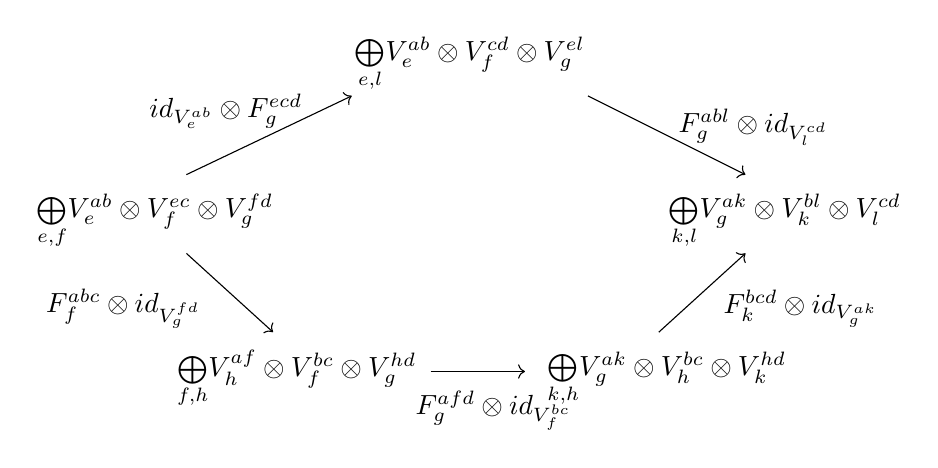
\begin{tikzpicture}
    \node at (0,-0.1) {$\underset{e,f}{\bigoplus} V^{ab}_e \otimes V^{ec}_f \otimes V^{fd}_g $};
    \draw[->, black] plot coordinates{(0.4,0.5) (2.5,1.5)};
    \node at (0.9,1.3) {$id_{V_{e}^{ab}} \otimes F^{ecd}_{g}$};
    \node at (4.0,1.9)  {$\underset{e,l}{\bigoplus} V^{ab}_e \otimes V^{cd}_{f} \otimes V^{el}_g$};
    \node at (7.6, 1.1) {$F^{abl}_{g} \otimes id_{V^{cd}_{l}}$};
    \draw[->] plot coordinates{(5.5, 1.5) (7.5,0.5)};
    \node at (8.0,-0.1) {$\underset{k,l}{\bigoplus} V^{ak}_{g} \otimes V^{bl}_{k} \otimes V^{cd}_{l}$};
    \node at (-0.4, -1.2) {$F^{abc}_{f} \otimes id_{V^{fd}_{g}}$};
    \draw[->] plot coordinates{(0.4,-0.5) (1.5,-1.5)};
    \node at (1.8,-2.1) {$\underset{f,h}{\bigoplus} V^{af}_{h} \otimes V^{bc}_{f}  \otimes V^{hd}_{g}$};
    \node at (4.3, -2.5) {$F^{afd}_{g} \otimes id_{V^{bc}_{f}}$};
    \draw[->] plot coordinates {(3.5,-2.0) (4.7, -2.0)};
    \node at (6.5, -2.1) {$\underset{k,h}{\bigoplus} V^{ak}_{g} \otimes V^{bc}_{h} \otimes V^{hd}_{k} $};
    \node at (8.2, -1.2) {$F^{bcd}_{k} \otimes id_{V^{ak}_{g}}$};
    \draw[->] plot coordinates {(6.4, -1.5) (7.5,-0.5) };
  \end{tikzpicture}
  \label{cat:pentagon}
  \end{gathered}
  \end{equation}
  The unit objects are given by 
\end{definition}

So far we have arrived at the structure of a fusion category. While we do not
have quantum systems based upon the objects of these categories, we can model
some processes through the hom-spaces, and we have $\C$-enrichment for them as
well. To model quantum systems, we need them to be Hilbert spaces as well.
Clasically this is done by defining a \emph{unitary structure} on the fusion
category. \todo{So why can we not jst do a Hilber-Enrichment?}

\todo{We could give this as a functor, but this has a weird target.}


\begin{definition}\label{cat:def:unitary}
  Let $\CC$ be a fusion category over $\C$. A \emph{\green{unitary structure}} on
  $\CC$ is a family of maps
  \[
    (-)^\dagger : \Hom_\CC(A,B) \to \Hom_\CC(B,A)
  \]
  which is the identity on objects and satisfies
  \begin{enumerate}
    \item \emph{(involution)} $(\lambda f + \mu g)^\dagger = \bar\lambda f^\dagger + \bar\mu g^\dagger$ and $f^{\dagger\dagger} = f$.
    \item \emph{(Contravariance)} $(f\circ g)^\dagger = g^\dagger \circ f^\dagger$ and $\id_A^\dagger = \id_A$.
    \item \emph{(Positivity)} $f^\dagger \circ f = 0 \implies f = 0$.
    \item \emph{(Monoidality)} $(f\ot g)^\dagger = f^\dagger \ot g^\dagger$, and the
      associator and unitors are unitary, e.g.\ $\alpha_{A,B,C}^\dagger = \alpha_{A,B,C}^{-1}$.
    \item \emph{(Duality)} the pivotal isomorphism $j_A : A \to A^{**}$ is
      unitary, equivalently $(f^\dagger)^* = (f^*)^\dagger$ for all $f$.
  \end{enumerate}
  A fusion category together with this structure is called a \emph{\green{unitary fusion category}}.
\end{definition}

\begin{proposition}
  In a unitary fusion category:
  \begin{enumerate}
    \item $\Hom_\CC(A,B)$ is a finite-dimensional Hilbert space for all $A,B$.
    \item The bases can be chosen with $\pi^{c,\mu}_{ab} =
      (\iota^{ab}_{c,\mu})^\dagger$, so each $\iota$ is an isometry, $\Phi$ is
      unitary, and $\iota\iota^\dagger$ is an orthogonal projection. The higher
      fusion-tree bases are orthonormal.
    \item The F-symbols $F^{abc}_d$ are unitary matrices.
    \item We can dfine an inner product on $\CC$ by
      \[
        \left\langle f, f\right\rangle = \tr(f^\dagger \circ f)
      \]
    \item Reciprocity $\Hom(R_c,R_a\ot R_b)\cong\Hom(R_a^*\ot R_c,R_b)$ is
      unitary up to the factor ???.
    \item If $\CC$ is braided with braiding $\beta$, then $\beta_{A,B}^\dagger =
      \beta_{A,B}^{-1}$ , so the R-symbols are unitary. In the ribbon case the
      twist satisfies $\theta_A^\dagger=\theta_A^{-1}$.
  \end{enumerate}
\end{proposition}

Now there is only one last structure missing before we can model anyons, and
this is perhaps the least intuitive of all of these structures. While
foundational for the physical interpretations of these theories, it is of little
interest to our tensor formalisms and we will not go into depth on this. 
\begin{definition}
  In a braided fusion category $\CC$ with $A,B \in \CC$ define the
  \emph{\green{S-matrix}}
  \[
    S_{AB} \coloneqq \tr(\beta_{B,A} \circ \beta{A,B}).
  \]
  If $S$ is invertible, we call the category \emph{\green{modular}}.
\end{definition}

\section{Decompositions for Categorical Networks}\label{cat:sub:decomp}

This chapter generalizes the decomposition in
\cite[Equation~27]{singhTensorNetworkStates2012a} to both Fusion Categories and the
Representation categories of compact groups. Note that in
\cite{devosTensorKitjlJuliaPackage2025}, such a generalization is given for
representations of finite groups, which does not include $SU(2)$. However I do not yet
know if we should do so, since I not yet sure how to argue the F moves here. If we instead
take the deformation $U_q(sl_2)$ we get finiteness (and fusion cats?), unfortunately
$U_q(sl_2)$ is not a group

\begin{definition}
  Recall that in a semisimple category $\CC$ we can express every object $S$ as a finite direct sum over isomorphism classes
  \[
    S \cong \bop_i S_i^{\op n_i}
  \]
  and we also work purely over $\C$ here. We now wish to mirror \emph{isotypic
  decomposition}\cref{sym:def:isotypic} within categories, i.e. we wish to
  categorify this construction. Let $V$ be a vector space of dimension $n$, i.e.
  choose a basis ${v_1, \ldots, v_n}$ and define
  \[
    V \iot C \coloneqq \bop_{i=1}^n C
  \]
  and we call $V$ the \emph{\green{multiplicity space}} of the object $C \in
  \CC$.
\end{definition}

Furthremore, we can assert that $- \iot - : \Veck \times \CC \to \CC$ is a
functor. 

\begin{lemma}\label{HomTensorFactorization}
Let $\CC$ be a $k$-linear category and let $D,E$ be finite-dimensional
$k$-vector spaces. For any objects $R,S\in \CC$, there is a natural
isomorphism
\[
\Hom_\CC(D \iot R,E \iot S)
\cong
\Hom_k(D,E)\otimes \Hom_\CC(R,S).
\]
\end{lemma}

\begin{proof}
Let $m=\dim_k D$ and $n=\dim_k E$. Proof by isomorphism chains: \todo{Redo this over a universal property, this is not natural.}
$$
  \begin{aligned}
    \Hom_C(D\otimes R,E\otimes S)
    &\cong \Hom_C(R^{\oplus m},S^{\oplus n})
    && \text{by \cref{lem:IsotopyHelper}} \\[1ex]
    &\cong \bigoplus_{i=1}^{m} \bigoplus_{j=1}^{n} \Hom_C(R,S)
    && \text{by additivity of $\Hom_C$} \\[1ex]
    &\cong k^{mn} \otimes \Hom_C(R,S)
    && \text{by \cref{lem:IsotopyHelper}} \\[1ex]
    &\cong \Hom_k(D,E)\otimes \Hom_C(R,S)
    && \text{since $\Hom_k(D,E) \cong k^{mn}$}
  \end{aligned}
$$
(The last as s)
\end{proof}

\begin{theorem}[Decomposition of Semisimple Categories]
  \label{DecompositionOfSemisimpleCategories}
  Let $C$ be a semisimple, monoidal, $k$-linear category whose tensor product is
  $k$-linear in each variable, with simple objects $\{R_a\}_{a\in L}$ and let $V_i, W_i$
  be a collection of (not necessarily simple) objects in $C$. Every morphism
  \[
    T \in \Hom_C\left(\bigot_{i = 1}^n V_i, \bigot_{i = 1}^m W_{i}\right)
  \]
  admit a decomposition as
  \[
    T \cong \bop_{\hat a,\hat b}
    \Hom_{k}(D_{\hat a}, E_{\hat b}) \ot_k \Hom_C(R_{\hat a},R_{\hat b}),
  \]
  where $\hat a = (a_1, \ldots , a_n )$ and $P$ is a $k$-vector space of dimension ???
\end{theorem}

\begin{proof}
\begin{align*}
\Hom_C&\!\left(
  \bigot_i V_i,
  \bigot_j W_j
\right) \\
&\cong
\Hom_C\!\left(
  \bigot_i
  \Bigl(
    \bop_{a_i}
    D_{i,a_i}\ot R_{a_i}
  \Bigr),
  \,
  \bigot_j
  \Bigl(
    \bop_{b_j}
    E_{j,b_j}\ot R_{b_j}
  \Bigr)
\right)
&\text{(\textcolor{gray}{\Cref{IsotopicDecomposition}})} 
\\[1.5ex]
&\cong
\Hom_C\!\left(
  \bop_{\hat a}
  D_{\hat a}\ot R_{\hat a},
  \,
  \bop_{\hat b}
  E_{\hat b}\ot R_{\hat b}
\right)
&\text{(\textcolor{gray}{linearity of $\ot$})}
\\[1.5ex]
&\cong
\bop_{\hat a,\hat b}
\Hom_C\!\left(
  D_{\hat a}\ot R_{\hat a},
  E_{\hat b}\ot R_{\hat b}
\right)
&
\text{\textcolor{gray}{(additivity of $\Hom_{\CC}$)}} 
\\[1.5ex]
&\cong
\bigoplus_{\hat a,\hat b}
\Hom\!\left(
  D_{\hat a},
  E_{\hat b}
\right)
\otimes
\Hom_C\!\left(
  R_{\hat a},
  R_{\hat b}
\right)
&\text{\textcolor{gray}{(\Cref{HomTensorFactorization})}} 
\end{align*}
In a basis expansion this then looks like
\[
  \cong
\bigoplus_{\hat a,\hat b}
\sum_{e,f,\mu,\nu}
\Hom\!\left(
  D_{\hat a},
  E_{\hat b}
\right)
\otimes_k
\mathsf{T}^{\widehat a,\widehat b}_{e,f;\mu,\nu}
\]
\end{proof}

\begin{corollary}[Operators are block matrices
\cite{kongInvitationTopologicalOrders2022b}] % TODO figure out why i cant cie theorems in
thm header.
  \label{cor:operator_blocks}
  An operator
  \[
    Hom(V,W) 
    \cong
    Hom_C\bigl(\bigoplus_a R_a^{\oplus d_a}, \bigoplus_b R_b^{\oplus e_b} \bigr) \cong \bigoplus_{a,b} Hom(D_a, E_b) \otimes Hom_C(R_a, R_b)
  \]
  and by Schurs lemma this is just
  \[
    \bigoplus_{a \in Irr(V) \cap Irr(W)} Hom(D_a, E_a) \cong \bigoplus_{a \in Irr(V) \cap Irr(W)} Mat_{d_a \times e_a}(k)
  \]
\end{corollary}

\begin{corollary}
  Let $Q_{\mu, \eta}$ be a basis of $Hom_C\bigl(\bigotimes_{\hat{a}} R_{\hat{a}},
  \bigotimes_{\hat{b} } R_{\hat{b} }  \bigr)$ where $\mu$ denotes the multiplicities and
  $\eta$ the internal fusions. In a \emph{multiplicity-free} Category we will omit $\mu$
  as a label. 
\end{corollary}

\begin{example}
  However, now assign $V_{\frac{1}{2}} \otimes V_{\frac{1}{2}}$ to each leg in the example
  above. Each leg then becomes $V_0 \oplus V_1 \cong \mathbb{C} \otimes V_0 \oplus
  \mathbb{C} \otimes V_1$. Then we can start with the decomposition.
  \[
    Hom_C(\bigoplus_{a,b,c \in (0,1)} (C \otimes C \otimes C) \otimes V_a \otimes V_b \otimes V_c, \bigoplus_{b \in (0,1)} C \otimes V_b) 
  \]
  \[
    = \bigoplus_{a,b,c,d \in (0,1)} Hom_C((C \otimes C \otimes C) \otimes (V_a \otimes V_b \otimes V_c), C \otimes V_d)
  \]
  \[
    = \bigoplus_{a,b,c,d} Hom(C^3, C) \otimes Hom_{\Rep(SU(2))} (V_a \otimes V_b \otimes V_c, V_d)
  \]
\end{example}

\begin{example}
  Easier. However, now assign $V_{\frac{1}{2}} \otimes V_{\frac{1}{2}}$ to each leg in the
  example above. Each leg then becomes $V_0 \oplus V_1 \cong \mathbb{C} \otimes V_0 \oplus
  \mathbb{C} \otimes V_1$. Then we can start with the decomposition.
  \[
    Hom_C\left(\bigoplus_{a,b\in (0,1)} (C \otimes C) \otimes V_a \otimes V_b \bigoplus_{b \in (0,1)} C \otimes V_b \right) 
  \]
  \[
    = \bigoplus_{a,b,c \in (0,1)} Hom_C((C \otimes C) \otimes (V_a \otimes V_b), C \otimes V_c)
  \]
  \[
    = \bigoplus_{a,b, c} Hom(C^2, C) \otimes Hom_{\Rep(SU(2))} (V_a \otimes V_b, V_c)
  \]
\end{example}

\begin{example}[XXZ-Hamiltonian]
  Consider a 4 leg tensor in $\End(V_{1/2} \ot V_{1/2})$, this decomposes as
  \[
A
  \]
\end{example}



\begin{example}
  Lets look at a tensor with in legs $(\tau \otimes \tau)$ and $\tau$ and out legs $\tau$.
  \[
    Hom_C(((k \otimes 1) \oplus (k \otimes \tau)) \otimes (k \otimes \tau), k\otimes\tau)
    =
    Hom_C()
  \]
  \[
    \begin{aligned}
      &\Hom_C\bigl(((k \otimes 1) \oplus (k \otimes \tau)) \otimes (k \otimes \tau),\, k\otimes\tau\bigr)\\
      &\cong
      \Hom_C\bigl((k\otimes1\otimes k\otimes\tau)
      \oplus
      (k\otimes\tau\otimes k\otimes\tau),\,k\otimes\tau\bigr)\\
      &\cong
      \Hom_C(k\otimes 1 \otimes k \otimes\tau,\,k\otimes\tau)
      \oplus
      \Hom_C(k\otimes \tau \otimes(k \otimes\tau),\,k\otimes\tau)\\
      &\cong
      \Hom(k \otimes k,k)\otimes\Hom_C(1 \otimes \tau,\tau)
      \oplus
      \Hom(k \otimes k,k)\otimes\Hom_C(\tau\otimes\tau,\tau).
    \end{aligned}
  \]
\end{example}

\begin{example}[Anyonic matrix operator]
  Finally, consider a $4 \to 4$ anyon operator with one leg on each side, representing the
  space $\mathrm{Hom}((\tau \otimes \tau \otimes \tau \otimes \tau), (\tau \otimes \tau
  \otimes \tau \otimes \tau))$. THe full decomposition is $2 + 3\tau$. Hence we obtain
  \[
    \Hom_C\!\left(
      (k^2 \otimes 1)\oplus(k^3\otimes\tau),
      (k^2 \otimes 1)\oplus(k^3\otimes\tau)
    \right).
  \]
  \[
    =
    \bigoplus_{a,b\in(1,\tau)}
    \Hom_C(k^{m_a}\otimes a,\,
    k^{m_b}\otimes b)
    =
    \bigoplus_{a,b\in(1,\tau)}
    \Hom(k^{m_a}, k^{m_b}) \otimes Hom_C(a,b)
  \]
  where
  \[
    m_1=2,
    \qquad
    m_\tau=3.
  \]
  For this case, Schurs lemma applies. So we have
  \[
    = Hom(k^2, k^2) \oplus Hom(k^3, k^3)
  \]
  which is just a block matrix with indexing $(1_1, 1_2, \tau_1, \tau_2, \tau_3)$.
\end{example}

\subsection{The Deligne Tensor Product \& Product Theories}
\label{subsect:deligne}



% https://q.uiver.app/#q=WzAsNSxbMCwyLCJcXGRpc3BsYXlzdHlsZVxcYmlnb3BsdXNfe2UsZn0gVl57YWJ9X2UgXFxvdGltZXMgVl57ZWN9X2YgXFxvdGltZXMgVl57ZmR9X2cgIl0sWzAsNCwiXFxkaXNwbGF5c3R5bGVcXGJpZ29wbHVzX3tmLGh9IFZee2FmfV9oIFxcb3RpbWVzIFZee2JjfV9mIFxcb3RpbWVzIFZee2hkfV9nICJdLFsyLDQsIlxcZGlzcGxheXN0eWxlXFxiaWdvcGx1c197ayxofSBWXntha31fZyBcXG90aW1lcyBWXntiY31faCBcXG90aW1lcyBWXntoZH1fayAiXSxbMSwwLCJcXGRpc3BsYXlzdHlsZVxcYmlnb3BsdXNfe2YsaH0gVl57YWZ9X2ggXFxvdGltZXMgVl57YmN9X2YgXFxvdGltZXMgVl57aGR9X2cgIl0sWzIsMiwiXFxkaXNwbGF5c3R5bGVcXGJpZ29wbHVzX3tmLGh9IFZee2FmfV9oIFxcb3RpbWVzIFZee2JjfV9mIFxcb3RpbWVzIFZee2hkfV9nICJdLFswLDEsIkZee2FiY31fZiBcXG90aW1lcyBpZF97Vl97Z31ee2ZkfX0iLDIseyJsYWJlbF9wb3NpdGlvbiI6NDB9XSxbMSwyLCJGXnthYmN9X2YgXFxvdGltZXMgaWRfe1Zfe2d9XntmZH19IiwyXSxbMCwzXSxbMyw0XSxbMiw0XV0=
\begin{tikzcd}
	& {\displaystyle\bigoplus_{f,h} V^{af}_h \otimes V^{bc}_f \otimes V^{hd}_g } & \\
	\\
	{\displaystyle\bigoplus_{e,f} V^{ab}_e \otimes V^{ec}_f \otimes V^{fd}_g } && {\displaystyle\bigoplus_{f,h} V^{af}_h \otimes V^{bc}_f \otimes V^{hd}_g } \\
	\\
	{\displaystyle\bigoplus_{f,h} V^{af}_h \otimes V^{bc}_f \otimes V^{hd}_g } && {\displaystyle\bigoplus_{k,h} V^{ak}_g \otimes V^{bc}_h \otimes V^{hd}_k }
	\arrow[from=1-2, to=3-3]
	\arrow[from=3-1, to=1-2]
	\arrow["{F^{abc}_f \otimes id_{V_{g}^{fd}}}"'{pos=0.4}, from=3-1, to=5-1]
	\arrow["{F^{abc}_f \otimes id_{V_{g}^{fd}}}"', from=5-1, to=5-3]
	\arrow[from=5-3, to=3-3]
\end{tikzcd}
\newpage

\chapter{Anyons II: Spin Chains \& Tensor Networks}
\label{sect:Anyons}
This chapter the diagrammatic methods that yield tensor networks on physical
systems that constitute \emph{anyons}. We introduce the fundamental theory of
anyons algebraically (\Cref{anyon:sec:algebraic_theory_of_anyons}), and make use
of the algebraic rules as the building blocks for our theory.
\Cref{anyon:sec:topology} gives examples of how the statistical properties of
anyons change with respect to it's ground state. Then, in
\Cref{anyon:sec:lattice_spin_chains}, we provide a worked examples of how anyons
are treated on \emph{spin-chains}, which motivates some aspect of the tensor
networks approach. TODO tensor network chapter. One of the primary motivations
for the study of anyons are their universality for quantum computation. In
\Cref{anyon:sec:tqc} we provide an interpretation of how both normal braiding
circuits and a variation in terms of \emph{weaves} can be simulated by the
tensor network theory.

\section{Algebraic Theory of Anyons}\label{anyon:sec:algebraic_theory_of_anyons}

Anyons are proposed as a \emph{defect} in a $2$ dimensional space (manifold? compact?)
with exotic exchange statistics. These exchange statistics differ from fermions in that we
allow particles to pick up a arbitrary phase $e^{i\theta}$ on exchange in the abelian
case, and a phase in a matrix element in the nonabelian case.

Generally when speaking about anyons, we group them into \emph{theories}. A anyon theory
is equipped with a (finite) set of charges $a,b,c,\ldots$ including a \emph{vacuum} charge
$I$. Additionally we are provided with a \emph{fusion rule} $a \times b = \sum_{c}^{}
N_{ab}^c c$ where $N_{ab}^c$ denotes the multiplicity. Since it can be shown (should I?)
that we cannot classify the vector space of two anyons $a,b$ by itself, we need to
parametrize this space over its \emph{fusion sectors}, i.e. the outcomes $c$ of the fusion
rule.

Consider an anyon to be a point-like defect on the plane carrying a charge out of the set
of labels. Since we need to reason about the properties of a pair of anyons using their
fusion-outcome, we draw this as follows:
%\[
%  \begin{tikzpicture}[scale=1.5]
%    \fill[gray!30] (3,0) ellipse (1 and 0.5);
%    \draw[->, thick] (3,0) ellipse (1 and 0.5);
%    \fill[white] (3.6,0) circle (0.1);
%    \draw[->, thick] (2.7,0) ellipse (0.6 and 0.3);
%    \node at (3.35,-0.2) {$1$};
%    \node[scale=2.5] at (2.4, 0) {$\cdot$};
%    \node at (2.5,0.1) {$\tau$};
%    \node[scale=2.5] at (3.0, 0) {$\cdot$};
%    \node at (3.1,0.1) {$\tau$};
%    \node[scale=2.5] at (3.6, 0) {$\cdot$};
%    \node at (3.7,0.1) {$\tau$};
%    \node at (4.0,-0.3) {$\tau$};
%\end{tikzpicture}
%\]
\[
  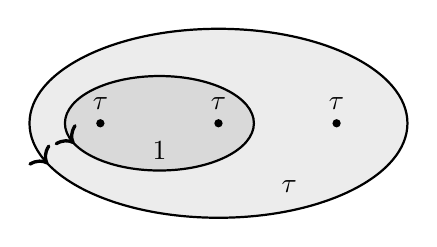
\begin{tikzpicture}[scale=1,
    ->-/.style={decoration={
      markings,
      mark=at position #1 with {\arrow[scale=1.5]{>}}},postaction={decorate}}
    ]

    \fill[gray!15] (1.5, 0) ellipse (2.4 and 1.2);
    \draw[thick, ->-=0.55] (1.5, 0) ellipse (2.4 and 1.2);
    \node at (2.4, -0.8) {$\tau$};

    \fill[gray!30] (0.75, 0) ellipse (1.2 and 0.6);
    \draw[thick, ->-=0.55] (0.75, 0) ellipse (1.2 and 0.6);
    \node at (0.75, -0.35) {$1$};

    \fill[black] (0, 0) circle (1.5pt);
    \node at (0, 0.25) {$\tau$};

    \fill[black] (1.5, 0) circle (1.5pt);
    \node at (1.5, 0.25) {$\tau$};

    \fill[black] (3.0, 0) circle (1.5pt);
    \node at (3.0, 0.25) {$\tau$};

\end{tikzpicture}
\]
The thick dark ellipses here denote the fusion outcome of two charges. Note that the line
here has an additional physical property in such that it is an \emph{observable}. This has
a nice interpretation in terms of bordisms: 

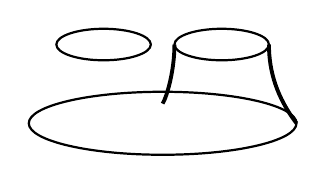
\begin{tikzpicture}
  \draw[thick] (3.25,0) ellipse (1.7 and 0.4);
  \draw[thick] (2.5,1) ellipse (0.6 and 0.2);
  \draw[thick] (4,1) ellipse (0.6 and 0.2);

  \draw[line width=1.4] (4.95, 0) .. controls (4.7, 0.33) and (4.6, 0.66) .. (4.6, 1);
  \draw[line width=1.4] (3.25, 0.25) .. controls (3.3, 0.33) and (3.4, 0.66) .. (3.4, 1);

\end{tikzpicture}

\[
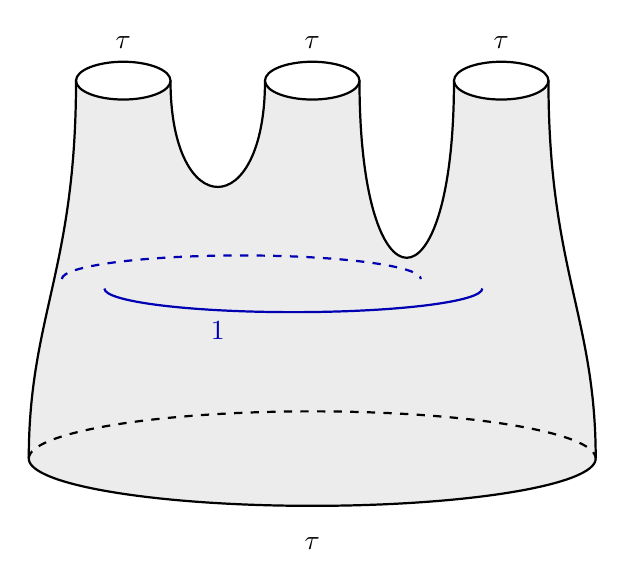
\begin{tikzpicture}[scale=1.2, thick]
    
    \fill[gray!15]
        (-2.5,0)
        .. controls (-2.5,1.5) and (-2,2) .. (-2,4)
        arc (180:360:0.5 and 0.2)
        .. controls (-1,2.5) and (0,2.5) .. (0,4) 
        arc (180:360:0.5 and 0.2)
        .. controls (1,1.5) and (2,1.5) .. (2,4)
        arc (180:360:0.5 and 0.2) 
        .. controls (3,2) and (3.5,1.5) .. (3.5,0) 
        arc (360:180:3.0 and 0.5);

    \draw (-2.5,0) .. controls (-2.5,1.5) and (-2,2) .. (-2,4);
    \draw (3.5,0)  .. controls (3.5,1.5) and (3,2) .. (3,4);
    
    \draw (-1,4) .. controls (-1,2.5) and (0,2.5) .. (0,4);
    \draw (1,4)  .. controls (1,1.5) and (2,1.5) .. (2,4);

    \draw[dashed, blue!70!black, thick] (-2.15, 1.9) arc (180:0:1.9 and 0.25);
    \draw[blue!70!black, thick] (-1.7, 1.8) arc (180:360:2.0 and 0.25
);
    \node[blue!70!black] at (-0.5, 1.35) {$1$};


    \fill[white] (-1.5,4) ellipse (0.5 and 0.2);
    \draw (-1.5,4) ellipse (0.5 and 0.2);
    \node at (-1.5, 4.4) {$\tau$};

    \fill[white] (0.5,4) ellipse (0.5 and 0.2);
    \draw (0.5,4) ellipse (0.5 and 0.2);
    \node at (0.5, 4.4) {$\tau$};

    \fill[white] (2.5,4) ellipse (0.5 and 0.2);
    \draw (2.5,4) ellipse (0.5 and 0.2);
    \node at (2.5, 4.4) {$\tau$};

    \draw[dashed] (-2.5,0) arc (180:0:3.0 and 0.5);
    \draw (-2.5,0) arc (180:360:3.0 and 0.5);
    \node at (0.5, -0.9) {$\tau$};

\end{tikzpicture}
\]



Let $V^{ab}_c$ be the space of 2 anyons of charges $a,b$ fusing to $c$. Then the

whole space $V^{ab}$ splits accordingly:
\[
  V^{ab} = \bigoplus_{c \in I} V^{ab}_c . 
\]
Since we wanted to assign meaning to the \emph{exchange} of particles, we define the exchange operator $R^{ab}$ componentwise:
\[
  R^{ab} : V^{ab} \to V^{ba}, \quad \bigoplus_c V^{ab}_c \cong \bigoplus_c V^{ba}_c.   
\]
as well as an isomorphism on combinations of more than $3$ particles
\[
  F^{abc} : V^{(ab)c} \cong V^{a(bc)}
\]

\subsection{Anyons on different topologies}\label{anyon:sec:topology}


\begin{figure}[h]
  \centering
  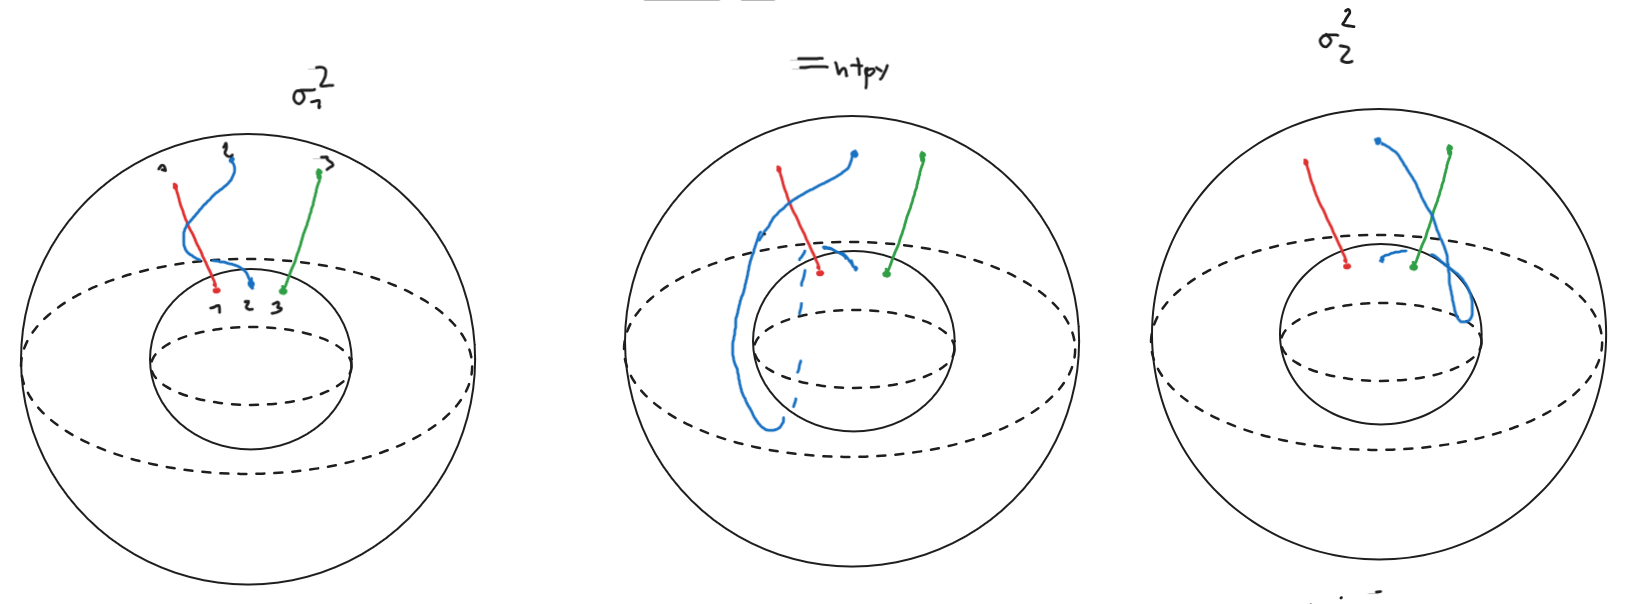
\includegraphics[width=0.8\textwidth]{figures/anyons_sphere.png}
  \caption{ $3$ Anyons on the sphere $S^2$ with the equivalence of the braids $\sigma_1^2$
    and $\sigma_2^2$. From an
    exercise\href{https://github.com/jkr11/maths-notes/tree/main/tq-simons-solutions}{github}
    in \cite{simonTopologicalQuantum2023}. }
  \label{anyon:fig:sphere}
\end{figure}

Analysing this case further yields that 
\[
  \pi_1(\mathrm{Conf}_3(S^2)) \cong Br(S^2) \cong \Z_4 \boxtimes \Z_3
\]
and thus finite. In fact, we know about the braid group on spheres that the order of
$Br_n(S^2)$ is given by
\begin{equation}
  \left\vert Br_n(S^2) \right\vert = \begin{dcases}
    \left\vert \Z_2 \right\vert = 2 &\text{ if } n = 2,\\
    \left\vert ??? \right\vert = 12  &\text{ if } n = 3, \\
    \infty &\text{ if } n \geq 4.
  \end{dcases}
  %\text{
  %  \stackrel{\cite[P~255]{fadellBraidGroupsE21962}}{\cite[Prop~2.2]{nlab:spherical_braid_group}}
  %}
  \shortstack[l]{
    \cite[p.~255]{fadellBraidGroupsE21962} \\
    \cite[Prop~2.2]{nlab:spherical_braid_group}
  }
\end{equation}


Also we should do or have done isotopy before. Technically the discussion here
also requires the completeness relations.

\begin{equation}\label{anyon:eq:complete}
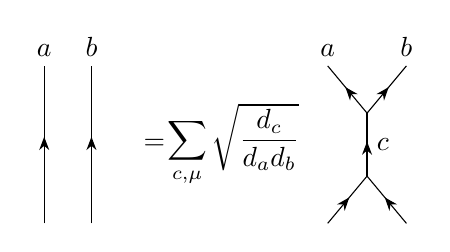
\begin{tikzpicture}[
    baseline=(current bounding box.center),
    scale=1.0,
    string arrow/.style={
        postaction={decorate},
        decoration={
            markings,
            mark=at position 0.55 with {\arrow[scale=1.0]{Stealth}}
        }
    }
  ]
  
  \draw[string arrow] (-2.5, 1.0) -- (-2.5, 3.0) node[above] {$a$};
  \draw[string arrow] (-1.9, 1.0) -- (-1.9, 3.0) node[above] {$b$};

  \node at (-1.1, 2.0) {$=$};
  \node at (-0.1, 2.0) {$\displaystyle\sum_{c,\mu} \sqrt{\frac{d_c}{d_a d_b}} $};

  \coordinate (bot_a) at (1.1, 1.0);
  \coordinate (bot_b) at (2.1, 1.0);
  
  \coordinate (mid_bot) at (1.6, 1.6);
  \coordinate (mid_top) at (1.6, 2.4);
  
  \coordinate (top_a) at (1.1, 3.0);
  \coordinate (top_b) at (2.1, 3.0);

  \draw[string arrow] (bot_a) -- (mid_bot);
  \draw[string arrow] (bot_b) -- (mid_bot);
  
  \draw[string arrow] (mid_bot) -- (mid_top) node[right, pos=0.5] {$c$};
  
  \draw[string arrow] (mid_top) -- (top_a) node[above] {$a$};
  \draw[string arrow] (mid_top) -- (top_b) node[above] {$b$};

\end{tikzpicture}
\end{equation}

\section{1D Lattice Models \& The Golden Chain}\label{anyon:sec:lattice_spin_chains}

%So from what i can read here (also the nlab or wikipedia) a spin chain specifically only
%refers to a per site construction with a tensor product hilbert space. An anyon chain is,
%well, an anyonic chain. These do not admit such a decomposition. So we should call these
%simply 1D lattice models.

What is a $2+1$D critical point? This is relevant for the distinction between
$1$D and $2$D models. Is a 2D model the same as a fusion surface model?

TODO: Write an outlook section here on work like
\cite{lootensDualitiesOnedimensionalQuantum2024}
\cite{eckQuantumLatticeModels2025} etc. This seems like a direct generalization
of our approach.

In \cite{feiguinInteractingAnyonsTopological2007}, anyonic chains, specifically in the
$\Fib$ model, are introduced as a $1$D lattice of $n$ $\tau$ anyons, defined as the fusion
space thereof.

\begin{tikzpicture}[
    baseline=(current bounding box.center),
    scale=1.2,
    string arrow/.style={
        postaction={decorate},
        decoration={
            markings,
            mark=at position 0.55 with {\arrow[scale=1.0]{Stealth}}
        }
    }
]
  \node (tleft) at (-3.9, 2.7) [left] {$\tau$};
  \node (t1) at (-3.2, 3.2) [above] {$\tau$};
  \node (t2) at (-2.5, 3.2) [above] {$\tau$};
  \node (t3) at (-1.8, 3.2) [above] {$\tau$};
  \node at (-0.5, 3.2) {$\cdots$};
  \node (tn1) at (0.8, 3.2) [above] {$\tau$};
  \node (tn) at (1.6, 3.2) [above] {$\tau$};

  \node (xi1) at (-3.2, 2.7) [inner sep=0pt, label=below:{$x_1$}] {};
  \node (xi2) at (-2.5, 2.7) [inner sep=0pt, label=below:{$x_2$}] {};
  \node (xi3) at (-1.8, 2.7) [inner sep=0pt, label=below:{$x_3$}] {};

  \draw [string arrow] (tleft) -- (xi1);
  \draw [string arrow] (t1) -- (xi1);

  \draw [string arrow] (t2) -- (xi2);
  \draw [string arrow] (xi1) -- (xi2);

  \draw [string arrow] (t3) -- (xi3);
  \draw [string arrow] (xi2) -- (xi3);

\end{tikzpicture}

Here, the state is fully characterized by its intermediate indeces $x_1 \ldots x_{n-1}$,
so we can choose a basis $\ket{x_1 x_2 \cdots x_{n-1} }$.

Similar to the Heisenberg-chain\footnote{Note that $\frac{1}{2} \otimes \frac{1}{2} = 0
\oplus 1$ in the Heisenberg $\SU 2$ model.}, the golden chain introduces a Hamiltonian
that assigns $-1$ to the interaction $\tau \otimes \tau = 1$ and $0$ to the interaction
$\tau \otimes \tau = \tau$.

We can decompose the whole space $\Hom(\tau^{\otimes n+1}, \tau)$ into the local states
\begin{equation}
  \Hom(\tau^{\otimes n+1}, \tau)
  =
  \bigoplus_{\mathclap{\substack{x_1, x_2, \ldots, x_{n-1} \\ \text{\color{RoyalBlue}{all admissible paths}}}}}
  \Hom(\tau \otimes \tau, x_1) \otimes \Hom(x_1 \otimes \tau, x_2)
  \otimes \cdots \otimes Hom(x_{n-1} \otimes \tau, \tau) 
\end{equation}
with the admissability condition that there are not adjacents $1$ in the sequence of
$x_i$s.

This is evaluated as a $3$ local hamiltonian, as we can decompose the spin chain into
local parts where two $\tau$ anyons are adjacent (check how they call it in the paper.).

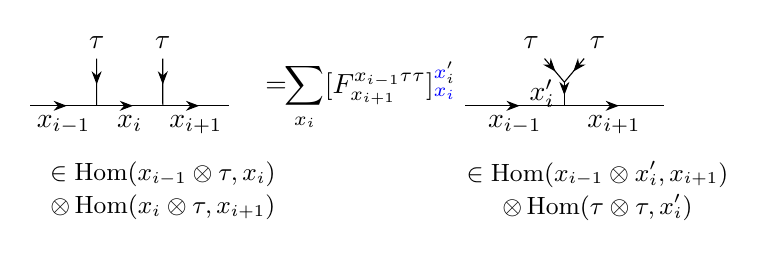
\begin{tikzpicture}[
    baseline=(current bounding box.center),
    scale=1.2,
    string arrow/.style={
        postaction={decorate},
        decoration={
            markings,
            mark=at position 0.55 with {\arrow[scale=1.0]{Stealth}}
        }
    }
]
  \coordinate (tleft) at (-3.9, 2.7);
  \node (t1) at (-3.2, 3.2) [above] {$\tau$};
  \node (t2) at (-2.5, 3.2) [above] {$\tau$};
  
  \coordinate (v1) at (-3.2, 2.7);
  \coordinate (v2) at (-2.5, 2.7);
  \coordinate (v3) at (-1.8, 2.7);

  \draw [string arrow] (tleft) -- node[below] {$x_{i-1}$} (v1);
  \draw [string arrow] (t1) -- (v1);

  \draw [string arrow] (v1) -- node[below] {$x_{i}$} (v2);
  \draw [string arrow] (t2) -- (v2);
  
  \draw [string arrow] (v2) -- node[below] {$x_{i+1}$} (v3);

  %\node (in1) at (-2.5, 2.0) {\tiny $\in Hom(x_{i-1} \otimes \tau, x_i)$ \\ $\otimes Hom(x_i \otimes \tau, x_{i+1} )$}; 
  \node (in1) at (-2.5, 1.8) [align=center] {
    \small $\in \Hom(x_{i-1} \otimes \tau, x_i)$ \\ 
    \small $\otimes \Hom(x_i \otimes \tau, x_{i+1})$
  };


  \node at (-1.3, 2.9) {$=$};
  \node at (-0.3, 2.8) {$\displaystyle\sum_{x_i} [F^{x_{i-1}\tau \tau }_{x_{i+1}}]_{\blue{x_i}}^{\blue x_i^\prime} $};

  \begin{scope}[xshift=4.6cm]
    \coordinate (rtleft) at (-3.9, 2.7);
    \node (rt1) at (-3.2, 3.2) [above] {$\tau$};
    \node (rt2) at (-2.5, 3.2) [above] {$\tau$};
    \coordinate (rtright) at (-1.8, 2.7);
    
    \coordinate (rvtau) at (-2.85, 2.95);
    
    \coordinate (rv1) at (-2.85, 2.7);

    \draw [string arrow] (rtleft) -- node[below] {$x_{i-1}$} (rv1);
    
    \draw [string arrow] (rt1) -- (rvtau);
    \draw [string arrow] (rt2) -- (rvtau);
    
    \draw [string arrow] (rvtau) -- node[left] {$x_{i}^\prime $} (rv1);
    
    \draw [string arrow] (rv1) -- node[below] {$x_{i+1}$} (rtright);

    \node (in1) at (-2.5, 1.8) [align=center] {
      \small $\in \Hom(x_{i-1} \otimes x_i^\prime , x_{i+1} )$ \\
      \small $\otimes \Hom(\tau \otimes \tau, x_{i}^\prime  )$
    }; 

  \end{scope}

\end{tikzpicture}

Now we can apply the interaction based on the intermediate state\footnote{Technically we
need a projector here read up again.} $x_i^\prime$ and apply another $F$-move back to the
chain basis:
$$
  H_{[i,i+1]} : 
  \ket{x_{i-1} x_i x_{i+1}  } \to \ket{x_{i-1} x_i^{\prime\prime} x_{i+1} } 
  \coloneqq
  \sum_{x_i^\prime \in \{1,\tau\} }^{} [F_{x_{i+1} }^{x_{i-1}\tau\tau}]_{x_i}^{x_i^\prime } 
    E_{x_{i}^\prime } 
    [F_{x_{i+1} }^{x_{i-1}\tau\tau }]_{x_{i^\prime }}^{x_{i^{\prime\prime}}}
  \label{anyon:eq:golden_chain_full}
$$
In the golden chain, we set $E_{1} = -1$ and $E_{\tau} = 0$. Then \eqref{anyon:eq:golden_chain_full} reduces to
\[
  H_{[i,i+1]} = - [F_{x_{i+1}}^{x_{i-1}\tau\tau}]_{x_i}^1 [F_{x_{i+1}}^{x_{i-1}\tau\tau}]_{1}^{x_{i}^{\prime\prime}}
\]

and we can write this three local hamiltonian as a matrix 
\[
  H_i = -J \begin{pmatrix}
    1 &  &  &  &   \\
     & 0 &  &  &   \\
     &  & 0 &  &   \\
     &  &  & \varphi^{-2}  & \varphi^{-\frac{3}{2}}  \\
     &  &  & \varphi^{-\frac{3}{2}} & \varphi^{-1}    \\
  \end{pmatrix}
\]


This method is reviewed and extended in \cite{trebstShortIntroductionFibonacci2008a}, with
longer ranger interaction. It will become apparent that the construction given in these
papers is a manualization of the tensor network constructions we will build here.
Generalizations to arbitrary models are given in \cite{gilsAnyonicQuantumSpin2013} as well
as \cite{buicanAnyonicChainsTopological2017}. Generalized spin chains and dualities using
module categories are given in \cite{eckQuantumLatticeModels2025}.

The tensor network formalism is handled in \cite{pfeiferSimulationAnyonsTensor2010},
\cite{pfeiferSimulationAnyonsUsing2012} and \cite{ayeniStudiesBraidedNonAbelian2017}, and
in terms of categories this is done in \cite{dissertation} and
\cite{devosTensorKitjlJuliaPackage2025}.


If we want to write this as a tensor contraction, we first define a hamiltonian
in a similar fashion to chapter 1. 

This takes the form of an operator in $Hom(\tau \otimes \tau, \tau \otimes \tau)$ as
\[
  \begin{tikzpicture}[scale=1.2,
    every node/.style={font=\small},
    fusion/.style={circle,fill=black,inner sep=1.2pt}
]

\node at (-2, 0.5) {$H_i = $};

\node at (-1, 0.5) {$E_1$};

\begin{scope}
  \node[fusion] (v1) at (0,0) {};
\node[fusion] (v2) at (0,1) {};

\draw (v1) -- (-0.7,-1);
\draw (v1) -- (0.7,-1);

\draw (v2) -- (0.7,2);
\draw (v2) -- (-0.7,2);

\draw (v1) -- (v2);

\node[left]  at (-0.7,-1) {$\tau$};
\node[right] at (0.7,-1) {$\tau$};
\node[left]  at (-0.7,2) {$\tau$};
\node[right] at (0.7,2) {$\tau$};

\node[left] at (-0.15,0.5) {$1$};

\end{scope}

\node at (1.5,0.5) {$+$};

\node at (2, 0.5) {$E_\tau$};

\begin{scope}[xshift=3cm]
  \node[fusion] (v1) at (0,0) {};
  \node[fusion] (v2) at (0,1) {};

  \draw (v1) -- (-0.7,-1);
  \draw (v1) -- (0.7,-1);

  \draw (v2) -- (0.7,2);
  \draw (v2) -- (-0.7,2);

  \draw (v1) -- (v2);

  \node[left]  at (-0.7,-1) {$\tau$};
  \node[right] at (0.7,-1) {$\tau$};
  \node[left]  at (-0.7,2) {$\tau$};
  \node[right] at (0.7,2) {$\tau$};

  \node[left] at (-0.15,0.5) {$\tau$};

\end{scope}

\end{tikzpicture}
\]
(Note this is allowed due to $\C$-linearity of $\Fib$.)


In this case we can view the golden chain approach chosen above as a manualization of the
tensor network process.

We can also write $H_i$ in its operator form matrix as
\[
  H_{i} \in \bigoplus_{a \in 1,\tau} Hom(\mathbb{C}, \mathbb{C})
\]
as 
\[
  H_i = -J \begin{array}{r@{\hspace{0.5em}}c}
  & \begin{array}{cc} 1 & \tau \end{array} \\
  \begin{array}{r} 1 \\ \tau \end{array} & 
  \begin{pmatrix}
   E_1 & 0\\
   0 & E_\tau   \\
  \end{pmatrix}
\end{array}
\]


\subsection{Topological Entanglement Entropy}

For simple lattice states, \cite{singhMatrixProductStates2014} defines a bipartition of
the lattice into anyons $A$ and $B$. Then we consider the whole space under charge
$a_{tot}$ as
\[
  V_{a_{tot}} = \bigoplus_{N_{ab}^{a_{tot} } = 1} (V^{A}_a \otimes V^{B}_b)
\] 
What i dont get here is why we are allowed to tensor both these sectors together without
the space $V_{ab}^{a_{tot} }$ explicitely.

TODO delete all of this and introduce this over the Hom category.

Anyhow, the fundamental building blocks we are using are the vector spaces $V^{ab}_c$
(where we refer to this as the fusion space from types $a$ and $b$ to $c$). This allows us
to build the vector space of two anyonic types $a,b$ as the sum over the fusion outcome:
\[
  V^{ab} = \bigoplus_{c \in Irr(C)} V^{ab}_c  
\]

We can directly introduce the $R$ move (a braiding of the initial anyons) to obtain the
isomorphic space $V^{ba}$ as
\[
  R : \bigoplus_{c \in Irr(C)} V^{ab}_c  \cong \bigoplus_{c \in Irr(C)} V^{ba}_c  
\] 

We can also write the space $V^{ab}_c = Hom(a \otimes b, c)$ in the categorical language.
Here we also need to realize that there is a difference between the isomorphism $\beta$
and the action of $R$, which is really on the hom space $\Hom(-, c)$. So this would be a
yoneda perspective? Since we know $R$ for all $a,b,c \in C$, we also know the action of
$R$ as an isomorphism. Well technically i believe that this allows us to determine for all
simples $c$, and then semisimplicity extends this to all subjects (this would be nice to
write down) and then the yoneda embedding is enough to know the whole space. Similarly, in
our Rep(G) categories (which i actually belive to be symmetric? Find this in etingof) 

The algebra-category correspondence in the theory of anyons was first noted by
\cite[App~E]{kitaevAnyonsExactlySolved2006}

\section{Topological Quantum Computation}\label{sect:anyon:tqc}

We want to build a quantum computer that acts purely on the topological data provided by the anyon theories, or as named by \textcite{freedmanNPQuantumField1998}, a \emph{Quantum Field Computer}. To do this we need 3 things:

\begin{enumerate}
  \item[] A ground state that has high enough dimension to represent a quantum bit, i.e. is $\cong \C^2$.
  \item[] A option to time evolve the system by application of unitaries.
  \item[] An option to read out the information of the evolved state (\emph{measurement}).
\end{enumerate}




Computing with nonabelian anyons requires a universal gate set built from representations
of the \emph{braid-group}:
\begin{definition}[Braid Group (algebraic)]
  \[
    Br(\R^2) 
    = 
    \left\langle 
      \begin{aligned}
      \sigma_i\sigma_j &= \sigma_j\sigma_i, \;\; \left\vert i - j \right\vert \geq 2\\
      \sigma_i\sigma_{i+1}\sigma_{i} &= \sigma_{i+1}\sigma_i\sigma_{i+1}, \;\; i \in [1,n-2]
    \end{aligned}
    \right\rangle
  \]
\end{definition}

and also the \emph{pure-braid-group}:

By the construction of anyon chains in \Cref{anyon:sec:algebraic_theory_of_anyons}, we know that the space of $3$ anyons fusing to $\tau$ is in fact $2$-dimensional. This motivates a choice of qubits as the following:

\begin{equation*}
  \vert 0 \rangle =
\raisebox{-20pt}{
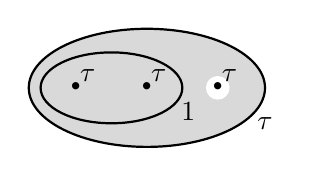
\begin{tikzpicture}[scale=1.5]
    \fill[gray!30] (3,0) ellipse (1 and 0.5);
    \draw[->, thick] (3,0) ellipse (1 and 0.5);
    \fill[white] (3.6,0) circle (0.1);
    \draw[->, thick] (2.7,0) ellipse (0.6 and 0.3);
    \node at (3.35,-0.2) {$1$};
    \node[scale=2.5] at (2.4, 0) {$\cdot$};
    \node at (2.5,0.1) {$\tau$};
    \node[scale=2.5] at (3.0, 0) {$\cdot$};
    \node at (3.1,0.1) {$\tau$};
    \node[scale=2.5] at (3.6, 0) {$\cdot$};
    \node at (3.7,0.1) {$\tau$};
    \node at (4.0,-0.3) {$\tau$};
\end{tikzpicture}
} 
\quad
\vert 1 \rangle = 
\raisebox{-20pt}{
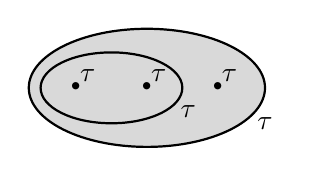
\begin{tikzpicture}[scale=1.5]    
    \fill[gray!30] (3,0) ellipse (1 and 0.5);
    \draw[thick] (3,0) ellipse (1 and 0.5);
    
    \draw[thick] (2.7,0) ellipse (0.6 and 0.3);
    \node at (3.35,-0.2) {$\tau$};

    \node[scale=2.5] at (2.4, 0) {$\cdot$};
    \node at (2.5,0.1) {$\tau$};
    \node[scale=2.5] at (3.0, 0) {$\cdot$};
    \node at (3.1,0.1) {$\tau$};
    \node[scale=2.5] at (3.6, 0) {$\cdot$};
    \node at (3.7,0.1) {$\tau$};
    \node at (4.0,-0.3) {$\tau$};
\end{tikzpicture}
}
\quad 
\vert NC \rangle =
\raisebox{-20pt}{
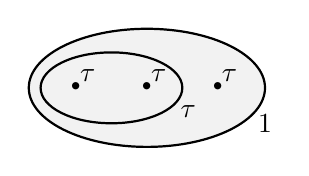
\begin{tikzpicture}[scale=1.5]

    \fill[gray!10] (3,0) ellipse (1 and 0.5);
    \draw[thick] (3,0) ellipse (1 and 0.5);
    
    \draw[thick] (2.7,0) ellipse (0.6 and 0.3);
    \node at (3.35,-0.2) {$\tau$};
    \node[scale=2.5] at (2.4, 0) {$\cdot$};
    \node at (2.5, 0.1) {$\tau$};
    \node[scale=2.5] at (3.0, 0) {$\cdot$};
    \node at (3.1,0.1) {$\tau$};
    \node[scale=2.5] at (3.6, 0) {$\cdot$};
    \node at (3.7,0.1) {$\tau$};
    \node at (4.0,-0.3) {$1$};

\end{tikzpicture}
}
\end{equation*}
and we say that $\C^2$ is \emph{embedded} in $V^{\tau \tau \tau}$. We could choose a different presentations, where each anyon is drawn from the vacuum as
\[
  TODO!
\]

Then we can build multi-qubit circuits by simply stacking these diagrams (inside their own fusion channel). This is what is called a \emph{sparse-encoding}. A dense encoding would correspond to just choosing the smallest space of appropriate dimension that includes one of the $(\C^2)^{\otimes d}$.

The solovay-kitaev theorem guarantees a polylog time and space algorithm for approximating
any gate in $\SU d$ to a desired accuracy. This, and similar procedures are realized by
the functor $\texttt{compile}$. A \emph{topological quantum compiler} essentially only
translates the qubits to their $\Hom$ space equivalences and translates the qudit-gates to
their braid group representations. There are of course special compilation methods, the
one we cover here takes first a decomposition of normal gates into CNOTs and then applies
injection weaving, so we only need to lower single qubit gates to braids.

% https://q.uiver.app/#q=WzAsNSxbMCwwLCIoXFxDXjIpXntcXG90aW1lcyBufSJdLFswLDIsIihcXENeMilee1xcb3RpbWVzIG59Il0sWzIsMiwiXFxIb20oXFx0YXVeezJuKzJ9LCBhKSJdLFsyLDAsIlxcSG9tKFxcdGF1XnsybiArIDJ9LCBhKSJdLFsxLDEsIlxcdGV4dHtDb21tdXRlcyB1cCB0b30gXFxcXCBcXHRleHR7Z2l2ZW4gfSBcXGVwc2lsb24gPSBcXHZlcnQgVSAtIFxccmhvKGIpIFxcdmVydCJdLFswLDMsIlxcdGV4dHR0e2NvbXBpbGV9Il0sWzEsMiwiXFx0ZXh0dHR7Y29tcGlsZX0iXSxbMywyLCJcXHJobyhiKSJdLFswLDEsIlUiLDJdXQ==
\[
\begin{tikzcd}
	{(\C^2)^{\otimes n}} && {\Hom(\tau^{2n + 2}, a)} \\
	& \begin{array}{c} \text{Commutes up to} \\ \text{given } \epsilon = \vert U - \rho(b) \vert \end{array} \\
	{(\C^2)^{\otimes n}} && {\Hom(\tau^{2n+2}, a)}
	\arrow["{\texttt{compile}}", hook, from=1-1, to=1-3]
	\arrow["U"', from=1-1, to=3-1]
	\arrow["{\rho(b)}", from=1-3, to=3-3]
	\arrow["{\texttt{compile}}", hook, from=3-1, to=3-3]
\end{tikzcd}
\]
Because this square commutes and $\texttt{compile}$ runs in polynomial time, we can in fact assert that the $QFC$ can simulate $BQP$.

However, compiling qudits for braids is a \emph{hard} (computationally
expensive) and slow process, as the dimension of the embedding is usually a
constant factor $> 1$ larger than the dimension of the desired qudit space. 

This process (and these do depend on the topology of the ground state) and the
indivuual gates are given in \cite{hadjiivanovBraidingFibonacciAnyons2024},
\cite{georgievDiagonalCosetApproach2024}.

The work of \textcite{simonTopologicalQuantumComputing2006a} provides a
alternative using the pure braid group. Remember that although we can represent any weave generator as 
\[
  T_{ij} = \sigma_i \sigma_{i+1} \cdots \sigma_{j-1} \sigma_{j}^2 \sigma_{j-1} \cdots \sigma_{i+1} \sigma_i
\]
a weave is effectively realized by moving only one of the particles (strands)
around $n-1$ fixed strands. As it turns out, the weave representations are also
dense in $\SU(2)$. (cite). This can also solve our problem of effectively
compiing controlled gates. Remember the presentation we chose for our qubits:
The $\ket{0}$ qubit has an intermediate channel of $1$ and the $\ket{1}$ qubit
has an intermediate channel of $\tau$. We also know that braiding a $1$-type
anyon around any other anyon shoulde have no effect. By our construction of
fusion we know that the tau anyons in the $1$ channel can only produce $1$ when
fused (i.e. $\tau \ot \tau = 1$). Should we have a superposition of qubits
$\alpha \ket{0} + \beta \ket{1}$ this means we produce a composite anyon of type
$0$ with probability $\alpha^2$ and a composite anyon of type $\tau$ with
probability $\beta^2$. Now if we find a weave realizing our controlled gate on
the lower qubit, we will have succesfully synthesized a controlled gate. For
this, we only need to \emph{inject} the composite anyon in the lower qubit
\emph{without} affecting the state of our system\todo{or doing so invertibly}.
After fusing in our top qubit, we effectively end up with a braiding problem in
$ \PBr_n$, however since we only want the $\tau$ part to have an effect we can
reduce this to $\Br_n$. Practically, this means that we need to find a
traditional braid $X \in Br_3$ such that the representation of 
\[
  \sigma_3
\]

We can use \emph{weaves} to build \emph{injection gates} which in
turn realize control gates. Then, by a universality argument of
\cite{freedmanModularFunctorWhich2000a} we can approximate any other multiqubit
gate, as single qubit gates can be computed in little time after an
algorithms\footnote{We provide an implementation of this process in
\texttt{Haskell} \cite{jeremiasJkr11Exactsynthhs2025} }\footnote{Although we
cannot reach the claimed bound of $\epsilon$ but instead reach
$\sqrt{\epsilon}$} of \cite{kliuchnikovAsymptoticallyOptimalTopological2013}
based on number theoretic methods (which are already mentioned in
\cite{freedmanLargeFourierTransforms2007}).\todo{Rewrite this.}

Specifically, there is a decomposition of an arbitrary gate in $(\C^{2})^{\ot
n}$ into a universal set of $CNOT$ and $\C^2$ unitaries. All that remains to do
is to reexpress a traditional working gate set in the $Fib$ basis of sets.

However we must also ensure that the decomposition in into CNOT does not produce
nonadjacent control-target pairs, as we can not freely cross the braids over
another qubit. This can however also be a problem for standard qubit
architectures, which is why we can decompose every unitary circuit into its
\emph{linear nearest neighbour} (LNN) form
\cite{kutinComputationDistance2007,saeediSynthesisQuantumCircuits2011}. Such
decompositions are already implemented in languages such as {\tt
Qiskit}\footnote{{\tt Qiskit} documentation:
\url{https://quantum.cloud.ibm.com/docs/en/api/qiskit}}\cite{javadiabhari2024quantum}.
%%%%%% This actually does not seem to be correct

\begin{figure}[h]
  
\vspace{.1cm}
\hspace{-1cm}
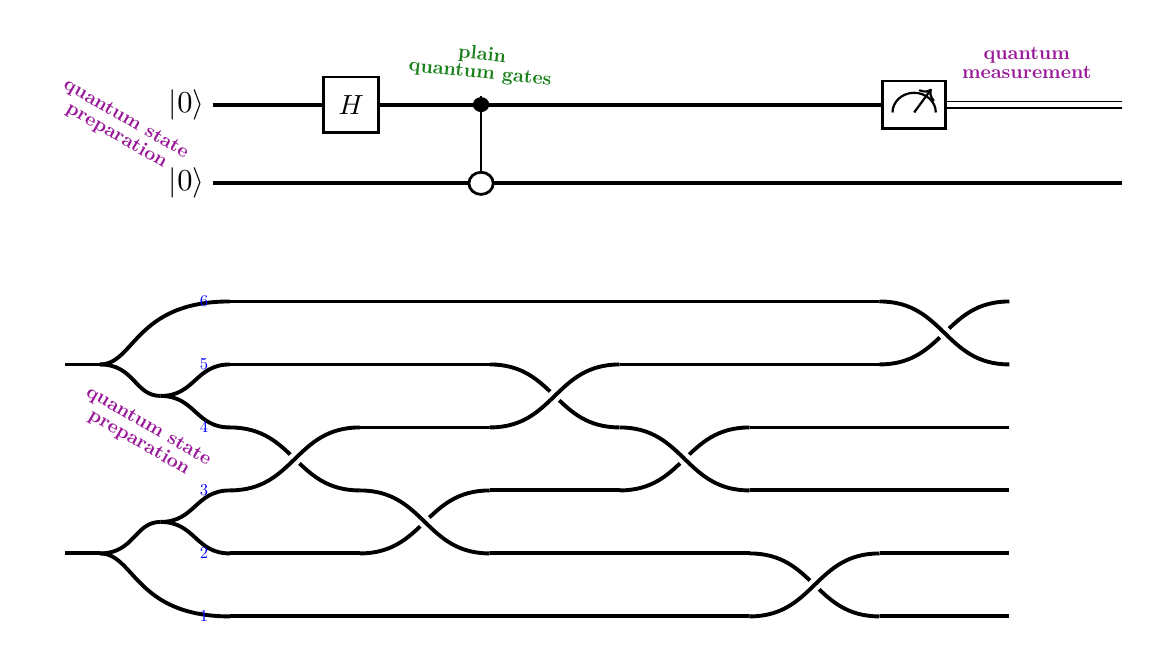
\begin{tikzpicture}[xscale={1.1}]

  \definecolor{purple}{rgb}{0.6, 0.1, 0.6}
  \definecolor{darkgreen}{rgb}{0.1, 0.5, 0.1}
  \definecolor{darkblue}{rgb}{0.1, 0.2, 0.7}

  \draw (-2.8, 0) node { \scalebox{1.1}{$\vert 0 \rangle$} };
  \draw (-2.8, -1) node { \scalebox{1.1}{$\vert 0 \rangle$} };

  \draw[line width=1.5pt] (-2.5,-1) to (+8,-1);
  \draw[line width=1.5pt] (-2.5,0) to (+5.5,0);

  \draw[line width=.6pt] (5.5,+.04) to (8,+.04);
  \draw[line width=.6pt] (5.5,-.04) to (8,-.04);

  \node[draw, fill=white, line width=1pt, minimum width=0.7cm, minimum height=0.7cm] (Hgate) at (-0.9, 0) {$H$};

  \draw[line width=1pt] (0.6, 0) -- (0.6, -1);
  \filldraw[black] (0.6, 0) circle (2.5pt);
  \draw[line width=1pt, fill=white] (0.6, -1) circle (4pt);
  \draw[line width=1pt] (0.6-4pt, -1) -- (0.6+4pt, -1);
  \draw[line width=1pt] (0.6, -1-4pt) -- (0.6, -1+4pt);

  \node[draw, fill=white, line width=1pt, minimum width=0.8cm, minimum height=0.6cm] (MeasBox) at (5.6, 0) {};
  \draw[line width=0.8pt] (5.6-0.25, 0-0.1) arc (180:0:0.25);
  \draw[line width=0.8pt, ->] (5.6, 0-0.1) -- (5.6+0.2, 0+0.2);

  \draw (-3.56, -.3) node[rotate=-30] {
    \scalebox{.7}{\color{purple}\bf\def\arraystretch{.8}\begin{tabular}{c}quantum state\\preparation\end{tabular}}
  };
  \draw (6.9, +.5) node {
    \scalebox{.7}{\color{purple}\bf\def\arraystretch{.8}\begin{tabular}{c}quantum\\measurement\end{tabular}}
  };
  \draw (1-.4, +.5) node[rotate=-6] {
    \scalebox{.7}{\color{darkgreen}\bf\def\arraystretch{.8}\begin{tabular}{c}plain\\quantum gates\end{tabular}}
  };


  \begin{scope}[shift={(-2.3, -4.5)}, rotate=90, yscale=1.0]

    \draw[line width=1.4] (-1.20, 1.90) to (-1.20, 1.50); 
    \draw[line width=1.4] (-1.20, 1.50) .. controls (-1.20, 1.10) and (-2.00, 1.10) .. (-2.00, 0.00); 
    \draw[line width=1.4] (-1.20, 1.50) .. controls (-1.20, 1.10) and (-0.80, 1.10) .. (-0.80, 0.80); 
    \draw[line width=1.4] (-0.80, 0.80) .. controls (-0.80, 0.40) and (-1.20, 0.40) .. (-1.20, 0.00); 
    \draw[line width=1.4] (-0.80, 0.80) .. controls (-0.80, 0.40) and (-0.40, 0.40) .. (-0.40, 0.00); 

    \draw (0.3,1) node[rotate=-30] {
      \scalebox{.7}{\color{purple}\bf\def\arraystretch{.8}\begin{tabular}{c}quantum state\\preparation\end{tabular}}
    };

    \draw[line width=1.4] (1.20, 1.90) to (1.20, 1.50); 
    \draw[line width=1.4] (1.20, 1.50) .. controls (1.20, 1.10) and (0.80, 1.10) .. (0.80, 0.80); 
    \draw[line width=1.4] (1.20, 1.50) .. controls (1.20, 1.10) and (2.00, 1.10) .. (2.00, 0.00); 
    \draw[line width=1.4] (0.80, 0.80) .. controls (0.80, 0.40) and (0.40, 0.40) .. (0.40, 0.00); 
    \draw[line width=1.4] (0.80, 0.80) .. controls (0.80, 0.40) and (1.20, 0.40) .. (1.20, 0.00); 

    \draw (-2.00, 0.3) node {\color{blue}\scalebox{.6}{1}};
    \draw (-1.20, 0.3) node {\color{blue}\scalebox{.6}{2}};
    \draw (-0.40, 0.3) node {\color{blue}\scalebox{.6}{3}};
    \draw (0.40, 0.3) node {\color{blue}\scalebox{.6}{4}};
    \draw (1.20, 0.3) node {\color{blue}\scalebox{.6}{5}};
    \draw (2.00, 0.3) node {\color{blue}\scalebox{.6}{6}};

    \draw[line width=1.4] (-2.00, 0.00) to (-2.00, -1.50);
    \draw[line width=1.4] (-1.20, 0.00) to (-1.20, -1.50);
    \draw[line width=1.4] (1.20, 0.00) to (1.20, -1.50);
    \draw[line width=1.4] (2.00, 0.00) to (2.00, -1.50);
    \draw[line width=1.4] (0.40, 0.00) .. controls (0.40, -0.75) and (-0.40, -0.75) .. (-0.40, -1.50);
    \draw[line width=4.5, white] (-0.40, 0.00) .. controls (-0.40, -0.75) and (0.40, -0.75) .. (0.40, -1.50);
    \draw[line width=1.4] (-0.40, 0.00) .. controls (-0.40, -0.75) and (0.40, -0.75) .. (0.40, -1.50);
    
    \draw[line width=1.4] (-2.00, -1.50) to (-2.00, -3.00);
    \draw[line width=1.4] (0.40, -1.50) to (0.40, -3.00);
    \draw[line width=1.4] (1.20, -1.50) to (1.20, -3.00);
    \draw[line width=1.4] (2.00, -1.50) to (2.00, -3.00);
    \draw[line width=1.4] (-1.20, -1.50) .. controls (-1.20, -2.25) and (-0.40, -2.25) .. (-0.40, -3.00);
    \draw[line width=4.5, white] (-0.40, -1.50) .. controls (-0.40, -2.25) and (-1.20, -2.25) .. (-1.20, -3.00);
    \draw[line width=1.4] (-0.40, -1.50) .. controls (-0.40, -2.25) and (-1.20, -2.25) .. (-1.20, -3.00);
    
    \draw[line width=1.4] (-2.00, -3.00) to (-2.00, -4.50);
    \draw[line width=1.4] (-1.20, -3.00) to (-1.20, -4.50);
    \draw[line width=1.4] (-0.40, -3.00) to (-0.40, -4.50);
    \draw[line width=1.4] (2.00, -3.00) to (2.00, -4.50);
    \draw[line width=1.4] (1.20, -3.00) .. controls (1.20, -3.75) and (0.40, -3.75) .. (0.40, -4.50);
    \draw[line width=4.5, white] (0.40, -3.00) .. controls (0.40, -3.75) and (1.20, -3.75) .. (1.20, -4.50);
    \draw[line width=1.4] (0.40, -3.00) .. controls (0.40, -3.75) and (1.20, -3.75) .. (1.20, -4.50);
    
    \draw[line width=1.4] (-2.00, -4.50) to (-2.00, -6.00);
    \draw[line width=1.4] (-1.20, -4.50) to (-1.20, -6.00);
    \draw[line width=1.4] (1.20, -4.50) to (1.20, -6.00);
    \draw[line width=1.4] (2.00, -4.50) to (2.00, -6.00);
    \draw[line width=1.4] (-0.40, -4.50) .. controls (-0.40, -5.25) and (0.40, -5.25) .. (0.40, -6.00);
    \draw[line width=4.5, white] (0.40, -4.50) .. controls (0.40, -5.25) and (-0.40, -5.25) .. (-0.40, -6.00);
    \draw[line width=1.4] (0.40, -4.50) .. controls (0.40, -5.25) and (-0.40, -5.25) .. (-0.40, -6.00);
    
    \draw[line width=1.4] (-0.40, -6.00) to (-0.40, -7.50);
    \draw[line width=1.4] (0.40, -6.00) to (0.40, -7.50);
    \draw[line width=1.4] (1.20, -6.00) to (1.20, -7.50);
    \draw[line width=1.4] (2.00, -6.00) to (2.00, -7.50);
    \draw[line width=1.4] (-1.20, -6.00) .. controls (-1.20, -6.75) and (-2.00, -6.75) .. (-2.00, -7.50);
    \draw[line width=4.5, white] (-2.00, -6.00) .. controls (-2.00, -6.75) and (-1.20, -6.75) .. (-1.20, -7.50);
    \draw[line width=1.4] (-2.00, -6.00) .. controls (-2.00, -6.75) and (-1.20, -6.75) .. (-1.20, -7.50);
    
    \draw[line width=1.4] (-2.00, -7.50) to (-2.00, -9.00);
    \draw[line width=1.4] (-1.20, -7.50) to (-1.20, -9.00);
    \draw[line width=1.4] (-0.40, -7.50) to (-0.40, -9.00);
    \draw[line width=1.4] (0.40, -7.50) to (0.40, -9.00);
    \draw[line width=1.4] (1.20, -7.50) .. controls (1.20, -8.25) and (2.00, -8.25) .. (2.00, -9.00);
    \draw[line width=4.5, white] (2.00, -7.50) .. controls (2.00, -8.25) and (1.20, -8.25) .. (1.20, -9.00);
    \draw[line width=1.4] (2.00, -7.50) .. controls (2.00, -8.25) and (1.20, -8.25) .. (1.20, -9.00);

  \end{scope}

\end{tikzpicture}
\caption{ A standard $2$-qubit quantum circuit and its lowering to a braid-circuit with
  inection weaves (missing yet).}
\end{figure}

\subsection{Application: Evaluating the Jones Polynomial}
\newpage

% \subsection{I dont know where to put this yet}

If we start out on anyonic chains, like the $SU(2)_3$ case, this provideds a nice generalization for chains with $C = Rep(SU(2)_k)$ with fusion rules
\[
  j_1 \times j_2 = \sum_{j = \left\vert j_1 - j_2 \right\vert }^{\mathop{\min}(j_1 + j_2, k - j_1 - j_2)} j.
\]
However now, if we approach this in the case of $SU(2)_\infty$ these fusion rules read
\[
  j_1 \times j_2 = \sum_{j = \left\vert j_1 - j_2 \right\vert }^{j_1 + j_2} 
\]
Is this the same as the Q deformations? It is for $q = 1$ and $k=\infty$ but what about the intermediates?

\section{MPO-symmetries}

So im not sure how this works completely but there seems to be way more literature on this than on (globally) symmetric tensors. However this also seems to be connected to anyonic networks. Also to the Category of MPS and MPO?

There is an account of (projective) representation on a peps that act on all levels in \cite{bridgemanEffectiveEdgeStates}. Actually there are more such as \cite[§~IV, Section~2]{cuiperHouchesLectureNotes2026}, \cite{williamsonMatrixProductOperators2016}

Some sources here: On Lattice Models with Module Categories: \cite{eckQuantumLatticeModels2025}, \cite{lootensDualitiesOneDimensionalQuantum2023} \cite{lootensDualitiesOneDimensionalQuantum2024} \cite{lootensEntanglementDensityMatrix2025}. Also chapters IV and V of \cite{cuiperHouchesLectureNotes2026}. On the structure see \cite{liuTradingMathematicalPhysical2025}

I think the original motivation for this is to have the following constraint on MPOs:

\[
  MPO_a \circ MPO_b = \sum_{c}^{} N_{ab}^c MPO_{c} 
\]
which we can obtain by a fusion tensor $X_{ab}^c$ that obeys an intertwining property. 

We immediately obtain our case of global symmetry by encoding
\[
  \rho(g) = \rho_1(g) \otimes \cdots \otimes \rho_n(g)
\]
as a MPO with bond dimension $1$ by setting 
\[
  W^{[a]}_{11,ij} = \rho_a(g)_{ij}
\]

Call $\rho(g) = MPO_g$. Then $\rho(g) \rho(h) = \rho(hg)$ 

If we want $MPO_g MPO_h = MPO_{hg}$ we also have MPO as a unitary representation with bond dimensions $ > 1$. So this generalizes the symmetry approach. 

TODO: check if we can give symmetries such as in the wanniers kramer dual that are given by $Z_i Z_{i+1}$ by not a $Rep(G)$ but instead a $Rep(\mathrm{G} )$ where $\mathrm{G} $ is a groupoid. 

\begin{definition}[2-Category of MPS]
  \label{def:mpsCategory}
  Let $A$ and $B$ be arbitrary MPS with bond collections $d^A, d^B$. Now, define the 1-morphism category $Hom(A \to B)$ where the objects are MPO operators $M$ together with a reduction isometry $Y$.
\end{definition}

I think we may be able to build a nice summary with this diagram:
% https://q.uiver.app/#q=WzAsMTIsWzAsMCwiKEFcXG90aW1lcyBCKVxcb3RpbWVzIEMiXSxbMiwwLCJBIFxcb3RpbWVzIChCIFxcb3RpbWVzIEMpIl0sWzAsMiwiSG9tKChBXFxvdGltZXMgQikgXFxvdGltZXMgQywgRCkiXSxbMiwyLCJIb20oQVxcb3RpbWVzIChCIFxcb3RpbWVzIEMpLCBEKSJdLFswLDUsIlxcZGlzcGxheXN0eWxlXFxiaWdvcGx1c19jIFZee0FCfV9jIFxcb3RpbWVzIFZee2NDfV9EIl0sWzIsNSwiXFxkaXNwbGF5c3R5bGVcXGJpZ29wbHVzX2MgVl57QWN9X0QgXFxvdGltZXMgVl57QkN9X2MiXSxbMSw0LCJcXGNvbmciXSxbMCw2LCJcXHVuZGVyc2V0e1xcYmx1ZXtcXG11IFxcaW4gMSxcXGxkb3RzLCBOXntBQn1fY30gXFxxdWFkIFxcYmx1ZXtcXG51IFxcaW4gMSxcXGxkb3RzLE5ee2NDLER9fX17XFx2ZXJ0IChBLEIpO2M7XFxtdVxccmFuZ2xlIFxcb3RpbWVzIFxcdmVydCBjLEM7IEQ7IFxcbnUgXFxyYW5nbGV9Il0sWzIsNiwiXFxkaXNwbGF5c3R5bGVcXHN1bV97ZixcXGFscGhhLFxcYmV0YX0gW0ZfRF57QUJDfV1feyhjXFxtdVxcbnUpfV57KGZcXGFscGhhXFxiZXRhKX0gXFx2ZXJ0IEEsZjtEO1xcYmV0YVxccmFuZ2xlIFxcb3RpbWVzIFxcdmVydCBCLEM7IGY7IFxcYWxwaGEgXFxyYW5nbGUiXSxbMCw0LCJcXGRpc3BsYXlzdHlsZVxcYmlnb3BsdXNfe2NcXGluIElycihDQVQpfSBIb20oQSBcXG90aW1lcyBCLCBjKSBcXG90aW1lcyBIb20oYyBcXG90aW1lcyBDLCBEKSJdLFsyLDQsIlxcZGlzcGxheXN0eWxlXFxiaWdvcGx1c197ZCBcXGluIElycihcXG1hdGhzZntDYXR9KX0gSG9tKEEgXFxvdGltZXMgZCwgRCkgXFxvdGltZXMgSG9tKEIgXFxvdGltZXMgQywgZCkiXSxbMSw1LCJcXGNvbmciXSxbMCwyLCJIb20oLSxEKSIsMV0sWzEsMywiSG9tKC0sRCkiLDFdLFswLDEsIlxcdW5kZXJzZXR7XFxzaW19e1xcYWxwaGFfe0FCQ319Il0sWzQsNywiXFxpbiIsMyx7InN0eWxlIjp7ImJvZHkiOnsibmFtZSI6Im5vbmUifSwiaGVhZCI6eyJuYW1lIjoibm9uZSJ9fX1dLFs3LDgsIlxcdW5kZXJzZXR7XFxncmVlbntcXHRleHR7Nmotc3ltYm9sc319fXtGXntBQkN9X0R9IiwxLHsic2hvcnRlbiI6eyJzb3VyY2UiOjEwLCJ0YXJnZXQiOjEwfX1dLFsyLDksIlxcdW5kZXJzZXR7XFx0ZXh0e1xcZ3JlZW57c2VtaXNpbXBsaWNpdHl9fX17XFxjb25nfSIsMyx7InN0eWxlIjp7ImJvZHkiOnsibmFtZSI6Im5vbmUifSwiaGVhZCI6eyJuYW1lIjoibm9uZSJ9fX1dLFszLDEwLCJcXHVuZGVyc2V0e1xcdGV4dHtcXGdyZWVue3NlbWlzaW1wbGljaXR5fX19e1xcY29uZ30iLDMseyJvZmZzZXQiOi0yLCJzdHlsZSI6eyJib2R5Ijp7Im5hbWUiOiJub25lIn0sImhlYWQiOnsibmFtZSI6Im5vbmUifX19XSxbOSw0LCI9IiwzLHsic3R5bGUiOnsiYm9keSI6eyJuYW1lIjoibm9uZSJ9LCJoZWFkIjp7Im5hbWUiOiJub25lIn19fV0sWzEwLDUsIj0iLDMseyJzdHlsZSI6eyJib2R5Ijp7Im5hbWUiOiJub25lIn0sImhlYWQiOnsibmFtZSI6Im5vbmUifX19XSxbNSw4LCJcXGluIiwzLHsic3R5bGUiOnsiYm9keSI6eyJuYW1lIjoibm9uZSJ9LCJoZWFkIjp7Im5hbWUiOiJub25lIn19fV0sWzIsMywiXFx1bmRlcnNldHtcXHNpbX17XFxhbHBoYV97QSxCLEN9fSJdLFsyLDMsIlxcc21hbGxcXGdyZWVue1xcdGV4dHthc3NvY2lhdG9yIGluZHVjZXMgaXNvbW9ycGhpbXMgdW5kZXIgeW9uZWRhfX0iLDAseyJvZmZzZXQiOjUsInN0eWxlIjp7ImJvZHkiOnsibmFtZSI6Im5vbmUifSwiaGVhZCI6eyJuYW1lIjoibm9uZSJ9fX1dXQ==
\[\begin{tikzcd}
	{(A\otimes B)\otimes C} && {A \otimes (B \otimes C)} \\
	\\
	{Hom((A\otimes B) \otimes C, D)} && {Hom(A\otimes (B \otimes C), D)} \\
	\\
	{\displaystyle\bigoplus_{c\in Irr(CAT)} Hom(A \otimes B, c) \otimes Hom(c \otimes C, D)} & \cong & {\displaystyle\bigoplus_{d \in Irr(\mathsf{Cat})} Hom(A \otimes d, D) \otimes Hom(B \otimes C, d)} \\
	{\displaystyle\bigoplus_c V^{AB}_c \otimes V^{cC}_D} & \cong & {\displaystyle\bigoplus_c V^{Ac}_D \otimes V^{BC}_c} \\
	{\underset{\blue{\mu \in 1,\ldots, N^{AB}_c} \quad \blue{\nu \in 1,\ldots,N^{cC,D}}}{\vert (A,B);c;\mu\rangle \otimes \vert c,C; D; \nu \rangle}} && {\displaystyle\sum_{f,\alpha,\beta} [F_D^{ABC}]_{(c\mu\nu)}^{(f\alpha\beta)} \vert A,f;D;\beta\rangle \otimes \vert B,C; f; \alpha \rangle} \\
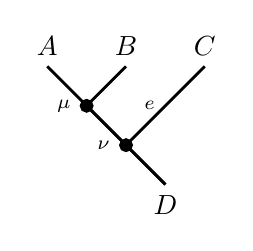
\begin{tikzpicture}[line width=1pt, node distance=1cm]
    % First diagram
    \coordinate (A) at (0,2);
    \coordinate (B) at (1,2);
    \coordinate (C) at (2,2);
    \coordinate (D) at (1.5,0.5);

    \coordinate (V1) at (0.5,1.5);
    \coordinate (V2) at (1.0,1);

    \draw (A) -- (D);
    \draw (B) -- (V1);
    \draw (V1) -- (V2);
    \draw (C) -- (V2);
    \draw (V2) -- (D);

    \filldraw (V1) circle (2pt) node[left=2pt,font=\scriptsize] {$\mu$};
    \filldraw (V2) circle (2pt) node[left=2pt,font=\scriptsize] {$\nu$};

    \node[above] at (A) {$A$};
    \node[above] at (B) {$B$};
    \node[above] at (C) {$C$};
    \node[below] at (D) {$D$};

    \node[left,font=\scriptsize] at (1.5,1.5) {$e$};
\end{tikzpicture}
& =  &
\hspace{-1.8cm}%
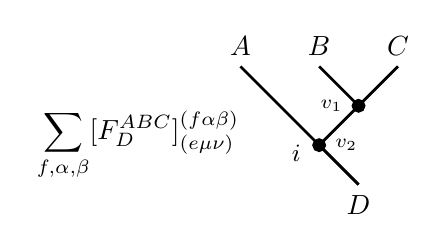
\begin{tikzpicture}[line width=1pt, node distance=1cm, xshift=-2cm]
    \begin{scope}[xshift=-2]
        
    \node at (-1.3,1) 
    {$\displaystyle\sum_{f,\alpha,\beta}
    [F^{ABC}_{D}]_{(e\mu\nu)}^{(f\alpha\beta)}$};

    \coordinate (A) at (0,2);
    \coordinate (B) at (1,2);
    \coordinate (C) at (2,2);
    \coordinate (D) at (1.5,0.5);

    \coordinate (V2) at (1.0,1);
    \coordinate (V1) at (1.5,1.5);

    \draw (A) -- (D);
    \draw (B) -- (V1);
    \draw (V1) -- (V2);
    \draw (C) -- (V1);
    \draw (V2) -- (D);

    \filldraw (V1) circle (2pt) node[left=2pt,font=\scriptsize] {$v_1$};
    \filldraw (V2) circle (2pt) node[right=2pt,font=\scriptsize] {$v_2$};

    \node[above] at (A) {$A$};
    \node[above] at (B) {$B$};
    \node[above] at (C) {$C$};
    \node[below] at (D) {$D$};

    \node[left,font=\small] at (0.9,0.9) {$i$};
    \end{scope}
\end{tikzpicture}
	\arrow["{\underset{\sim}{\alpha_{ABC}}}", from=1-1, to=1-3]
	\arrow["{Hom(-,D)}"{description}, from=1-1, to=3-1]
	\arrow["{Hom(-,D)}"{description}, from=1-3, to=3-3]
	\arrow["{\underset{\sim}{\alpha_{A,B,C}}}", from=3-1, to=3-3]
	\arrow["{\green{\text{associator induces isomorphims under yoneda}}}", shift right=5, draw=none, from=3-1, to=3-3]
	\arrow["{\underset{\text{\green{semisimplicity}}}{\cong}}"{marking, allow upside down}, draw=none, from=3-1, to=5-1]
	\arrow["{\underset{\text{\green{semisimplicity}}}{\cong}}"{marking, allow upside down}, shift left=2, draw=none, from=3-3, to=5-3]
	\arrow["{=}"{marking, allow upside down}, draw=none, from=5-1, to=6-1]
	\arrow["{=}"{marking, allow upside down}, draw=none, from=5-3, to=6-3]
	\arrow["\in"{marking, allow upside down}, draw=none, from=6-1, to=7-1]
	\arrow["\in"{marking, allow upside down}, draw=none, from=6-3, to=7-3]
	\arrow["{\underset{\green{\text{6j-symbols}}}{F^{ABC}_D}}"{description},  from=7-1, to=7-3]
\end{tikzcd}\]


\appendix
\chapter{Appendix}

\section{Some Group Theory}
\label{app:gen:groups}

\begin{definition}
    A \emph{\green{group}} $(G,\cdot)$ consists of a (possibly infinite) set of
    elements and a binary op $\cdot : G \times G \to G$ such that
    \begin{enumerate}
        \item $(a \cdot b) \cdot c = a \cdot (b \cdot c)$
        \item There exists an $\id_G \in G$ s.t. $\id_G \cdot\;a = a \cdot \id_G = a$
        \item Each $a \in G$ is invertible with $a \cdot a^{-1} = a^{-1} a =
        \id_G$
    \end{enumerate}
\end{definition}

\begin{definition}
    A group $(G,\cdot)$ is called \emph{\green{abelian}}, if for all $a,b \in G$
    it holds that $a \cdot b = b \cdot a$, its contrapose is called a
    \emph{\green{non-abelian}} group.
\end{definition}

Recall that we say a group is \emph{generated} by a set of elements if we can
write any other element as the concatenation of the generating set. Here by
example:

\begin{definition}
    The \emph{\green{symmetric group}} of $n$ points $S_n$ is given by
    \begin{equation}
        S_n 
        = 
        \left\langle 
        s_1, \ldots, s_{n-1} 
        \;\middle\vert\;    
        \begin{aligned}
            s_i^2 &= id \\
            s_i s_{i+1} s_i &= s_{i+1} s_i s_{i+1} \\
            s_i s_j &= s_j s_i, \vert i - j \vert \geq 2
        \end{aligned}
        \;\right\rangle.
    \end{equation}
\end{definition}

\begin{definition}[Representation theory of the symmetric group]
    For $n \geq 2$ the symmetric group $S_n$ is equipped with two
    one-dimensional representations, the \emph{trivial representation} where
    every generator is equal to the identity, and the \emph{sign representation}
    which equips each generator with its relative permutation parity.
\end{definition}

\begin{definition}
    The \emph{\green{General Linear Group}} $\GL{n}$ of degree $n$ is the set of
    $n\times n$ matrices that are invertible, and its operation $\cdot$ is that
    of matrix multiplication. 
\end{definition}

\section{Some Algebraic Topology}
\label{app_gen:homotopy}

Let spaces $X,Y$ be topological in the following, and let all functions be
continuous unless stated otherwise.

\begin{definition}
    A \emph{\green{homotopy}} between two continuous functions $f,g : X \to Y$
    is a continuous function
    \begin{equation}
        H : X \times [0,1] \to Y \text{ such that } H(x,0) = f(x) \text{ and } H(x,1) = g(x)
    \end{equation}
\end{definition}

\begin{definition}
    A \emph{\green{loop}} with basepoint $x_0$ on $X$ is a function
    \begin{equation}
        \gamma : [0,1] \to X \quad \text{such that} \gamma(0) = \gamma(1) = x_0
    \end{equation}
\end{definition}

\section{Proofs for \Cref{sect:symmetricTensorNetworks}}
This is the proof for statement \Cref{sym:eq:u1_commutes} on page \pageref{sym:eq:u1_commutes}.

\begin{lemma}
  The $XXZ$ Hamiltonian admits a symmety under $U(\theta) = e^{i\theta S_{tot}^z }$ and diagonalizing with $S_{tot}^z$ suffices. 
\end{lemma}

\begin{proof}\label{app:proof:u1_commutes}
  Actually should we just cite a proof or is this of interest? \cite[§~4.2]{Hassler2024}.
  Recall that when two operators commute, we can \emph{simultaneously diagonalize} them
  \cite[Theorem~1.3.12]{Horn_Johnson_2012}.

  \begin{align*}
    [H, S^z_{\mathrm{tot}}] = \sum_{i}^{N} [\sigma_i^x \sigma_{i+1}^x + \sigma_i^y \sigma_{i+1}^y + \Delta \sigma_i^z \sigma_i^z, \sum_{j = 1}^{N} \sigma_j^z ] 
  \end{align*}
  and since operators on different sites commute, only $j = i$ and $j = i+1$ contribute.
  So we ought to write
  \[
    \sum_{i}^{N} [\sigma_i^x \sigma_{i+1}^x + \sigma_i^y \sigma_{i+1}^y + \Delta \sigma_i^z \sigma_i^z, \sigma_i^z + \sigma_{i+1}^z  ] 
  \]
  and now using the identity $[AB,C] = A[B,C] + [A,C]B$:
  \[
    [\sigma_i^x \sigma_{i+1}^x, \sigma_i^z + \sigma_{i+1}^z  ] = -2i(\sigma_i^y \sigma_{i+1}^x + \sigma_i^x \sigma_{i+1}^y  ) 
  \]
  \[
    [\sigma_i^y \sigma_{i+1}^y, \sigma_i^z + \sigma_{i+1}^z  ] = 2i(\sigma_i^x \sigma_{i+1}^{y} + \sigma_i^y \sigma_{i+1}^x  )
  \]
  which cancel out. Furtermore, the $z$ spins commute as well. Thus the whole sum is $0$
  and we are done.
\end{proof}



\section{Supplementary categorical constructions for \Cref{sect:Categories}}
Note on universal properties: When dealing with categories, we are fundamentally dealing with abstractions that behave alike to a known construction. These behaviours are made precise by the use of a \emph{universal property}. We illustrate this with the definition of a (co)product: 

\begin{definition}\label{app:def:product_coproduct}
  Let $\CC$ be a category and $x,y \in ob(\CC)$. Their \emph{\green{product}} is an object $x \prod y$ in $\CC$ with morphisms $\pi_x : x \prod y \to x$ and $\pi_y : x \prod y \to y$. Their \emph{\green{coproduct}} is defined as the object $x \coprod y$ together with the maps $\iota_x : x \to x \coprod y$ and $\iota_y : y \to x \coprod y$. Both of these definitions are universal with their properties. 
  % https://q.uiver.app/#q=WzAsOCxbMSwxLCJ4IFxccHJvZCB5Il0sWzEsMiwieCJdLFsyLDEsInkiXSxbNCwxLCJ4XFxjb3Byb2QgeSJdLFswLDAsIloiXSxbMywwLCJaXlxccHJpbWUiXSxbNCwyLCJ4Il0sWzUsMSwieSJdLFswLDEsIlxccGlfeCJdLFswLDIsIlxccGlfeSIsMl0sWzQsMiwiXFxwaV5cXHByaW1lX3kiXSxbNCwxLCJcXHBpX3heXFxwcmltZSIsMl0sWzQsMCwiXFxleGlzdHMhIiwxXSxbNyw1LCJcXGlvdGFfeSIsMl0sWzYsNSwiXFxpb3RhX3giXSxbNywzLCJcXGlvdGFfeSJdLFs2LDMsIlxcaW90YV94IiwyXSxbMyw1LCJcXGV4aXN0cyEiLDEseyJzdHlsZSI6eyJ0YWlsIjp7Im5hbWUiOiJhcnJvd2hlYWQifSwiaGVhZCI6eyJuYW1lIjoibm9uZSJ9fX1dXQ==
  \[\begin{tikzcd}
	  Z &&& {Z^\prime} && \\
	  & {x \prod y} & y && {x\coprod y} & y \\
	  & x &&& x
	  \arrow["{\exists!}"{description}, from=1-1, to=2-2]
	  \arrow["{\pi^\prime_y}", from=1-1, to=2-3]
	  \arrow["{\pi_x^\prime}"', from=1-1, to=3-2]
	  \arrow["{\pi_y}"', from=2-2, to=2-3]
	  \arrow["{\pi_x}", from=2-2, to=3-2]
	  \arrow["{\exists!}"{description}, from=1-4, to=2-5]
	  \arrow["{\iota_y}"', from=2-6, to=1-4]
	  \arrow["{\iota_y}", from=2-6, to=2-5]
	  \arrow["{\iota_x}", from=3-5, to=1-4]
	  \arrow["{\iota_x}"', from=3-5, to=2-5]
  \end{tikzcd}\]
\end{definition}


This should all go in the anyon chapter? or later on into categories. Lets show
how to build the splitting of a fusion tree 
\[
  \Hom(a \otimes b \otimes d, e) = \bigoplus_c \Hom(a \otimes b, c) \otimes \Hom(c \otimes d, e)
\]

First we ought to give an mapping 
\[
  \Theta_c : \Hom(a \ot b, c) \ot_k \Hom(c \ot d, e) \to \Hom(a \otimes b \otimes d, e)
\]
by
\[
  \mu \ot_k \nu \mapsto (\mu \otimes \id_d) \circ \nu
\]  

\subsection{TQFT}

Hmm, where does this go?

A TQFT is defined by a finite set of labels $L$, and a rule that assigns each
compact cpa-space a vector space and each map between them (a cobordism) a
linea map between spaces. A TQFT is thus a functor between the category $(Bord,
\sqcup, \emptyset) \to \mathrm{Vect}$.

We can interpret this as assigning each ??? bordism its space of states under
the functor and each cobordism its space of operators.



\section{Overview of existing implementations}
% sources for R and TM symbols:
% https://tex.stackexchange.com/questions/168938/how-to-insert-a-trademark-symbol-tm
% https://tex.stackexchange.com/questions/1676/how-to-get-good-looking-copyright-and-registered-symbols
% From package managers a la carge (arxiv:2602.18602v5) table.tex
\newcounter{tabfn}
\newcommand{\crs}{\color{black}{\ding{55}}}

\newcommand{\tfntext}[2]{%
  \refstepcounter{tabfn}%
  \noindent\textsuperscript{\arabic{tabfn}}%
  \raisebox{7pt}[0pt][0pt]{\phantomsection\label{tabfn-#1}}%
  #2\par
}
\newcommand{\tfnref}[1]{\hyperref[tabfn-#1]{\textsuperscript{\ref{tabfn-#1}}}}

\newcommand\bcircle[2][]{\ifmmode
    \Circled[fill color=white,inner color=black,#1]{\mathsf{#2}}
  \else
    \Circled[fill color=white,inner color=black,#1]{\sffamily#2}
  \fi
}

\newcommand{\cL}{\bcircle{L}} % Library
\newcommand{\cB}{\bcircle{B}} % Backend / Extension
\newcommand{\cR}{\bcircle{R}} % Research Code / standalone script

%\begin{table}[h]
%\centering
%\rowcolors{2}{gray!10}{white}
%\begin{tabularx}{\textwidth}{l l X l}
%\hline
%\textbf{Software} & \textbf{Symmetry} & \textbf{Citation (Software, Publication)} & \textbf{Language} \\
%\hline
%ITensor & Nonabelian (Fermion?) & \cite{fishmanITensorSoftwareLibrary2022} & Julia \\
%Cyten & Categorical & \cite{unfriedCyten}, \cite{dissertation} & Python \& C++ \\
%TeNPy & Abelian & \cite{hauschildTensorNetworkPython2024} & Python \\
%QSpace & Nonabelian & \cite{weichselbaumQSpaceOpensourceTensor2024}, \cite{weichselbaumNonabelianSymmetriesTensor2012} & ? \\
%ChemTensor & $\SU{2}$ & \cite{QctumChemtensor2026} & C \\
%UniTensor & ? & \cite{} & ? (Python, C++) \\
%YASTN & Abelian & \cite{ramsYASTNAnotherSymmetric2025} & Python \\
%TensorKit.jl\footnotemark & Categorical & \cite{devosTensorKitjlJuliaPackage2025} & Julia \\
%Cytnx & Abelian only (?) & \cite{} & C++ \\
%quimb & Fermion? & \cite{} & Python \\
%MPSKit.jl & (similar to TensorKit?) & \cite{} & Julia \\
%TeMFpy & Fermion? & \cite{temfpy} & Python \\
%abeliantensors & $\U{1}$ and $\mathbb{Z}_n$ & \cite{hauruMhauruAbeliantensors2026} & Python \\
%symmray & Fermion & \cite{gaoFermionicTensorNetwork2025}, \cite{grayJcmgraySymmray2026} & ? \\
%grassmanntn & Grassmann & \cite{yosprakobAyosprakobGrassmanntn2026} & ? \\
%SymLibrary & ? (on-site) & \cite{mcmahonQnlaSymLibrary2019}, \cite{mcmahonHolographicDualityLifted2020} & MATLAB? \\
%%Telum.jl & Nonabelian & \cite{leeSsbleeTelumjl2026} & Julia \\
%%Su2tn & $\SU{2}$ & \cite{fischerVictorfischer2000Su2tn2025}, \cite{fischerTensorNetworkSymmetries2025} & Python \\
%%\hline
%%\end{tabularx}
%%\captionsetup{justification=centering}
%%\caption{Overview of tensor network libraries and symmetry support. (There are some closed-source things here as well; also, what is the software used by Singh et al.?) Software is included if it has a website or documentation and an account of the symmetries it exploits. Applications or theory are listed in the Citation column.}
%%\label{tab:tn-libraries}
%%\end{table}
%%\footnotetext{Part of the \texttt{QuantumKit.jl} ecosystem.}
%%
%%\newpage
%
%\newpage
%\begin{landscape}
%
%\begin{table}[h]
%\centering
%\small
%\label{tab:tn-libraries}
%
%\captionsetup{justification=centering}
%\caption{Overview of tensor network libraries and their support for symmetries.
%If a specific symmetry is given, the software is restricted to that symmetry. A
%previous list of existing implementations in 2018 is also given in
%\cite{hubigGlobalSymmetriesTensora}. }
%\rowcolors{2}{gray!10}{white}
%\begin{tabularx}{\textwidth}{l c l | c c c c c}
%\rowcolor{white}
%\textbf{Software}
%& \textbf{Year}
%& \textbf{Language}
%& \makecell{\textbf{Abelian}\\ \S\ref{sect:symmetricTensorNetworks}}
%& \makecell{\textbf{Non-Abelian} \\ \S\ref{sect:symmetricTensorNetworks}}
%& \makecell{\textbf{Categorical} \\ \S\ref{sect:Categories}}
%& \makecell{\textbf{Product}\\\textbf{Symmetries} \\ \S\ref{subsect:deligne}}
%& \textbf{\makecell{Software \& \\ Publication}}
%\\[-1mm]
%\hline
%
%ITensor
%& 2022
%& Julia
%& $\checkmark$
%& $\checkmark$
%& ?
%& ?
%& \cite{fishmanITensorSoftwareLibrary2022}
%\\
%
%Cyten\tfnref{cyten}\tfnref{cytnx}
%& 2024
%& Python \& C++
%& $\checkmark$
%& $\checkmark$
%& $\checkmark$
%& $\checkmark$
%& \cite{unfriedCyten}, \cite{dissertation}
%\\
%
%TeNPy
%& 2019 % what is this actually? first stable release?
%& Python
%& $\checkmark$
%& 
%& 
%& ?
%& \cite{hauschildTensorNetworkPython2024}
%\\
%
%QSpace
%& 2012
%& ?
%& $\checkmark$
%& $\checkmark$
%& $\crs$
%& ?
%& \cite{weichselbaumQSpaceOpensourceTensor2024},
%  \cite{weichselbaumNonabelianSymmetriesTensor2012}
%\\
%
%SyTen
%& 2017
%& C++
%& ?
%& ?
%& ?
%& ?
%& \cite{hubig:_syten_toolk,hubig17:_symmet_protec_tensor_networ} \\
%
%ChemTensor
%& 2023
%& C
%& $\checkmark$
%& $\mathrm{SU}(2)$
%& $\crs$
%& ?
%& \cite{QctumChemtensor2026}
%\\
%
%Uni10
%& 2015
%& Python, C++
%& ?
%& ?
%& ?
%& ?
%& \cite{kaoUni10OpensourceLibrary2015}
%\\
%
%YASTN
%& 2025
%& Python
%& $\checkmark$
%& 
%& 
%& ?
%& \cite{ramsYASTNAnotherSymmetric2025}
%\\
%
%TensorKit.jl\tfnref{tensorkit}
%& 2025
%& Julia
%& $\checkmark$
%& $\checkmark$
%& $\checkmark$
%& $\checkmark$
%& \cite{devosTensorKitjlJuliaPackage2025}
%\\
%
%Cytnx\tfnref{cytnx}
%& 2024
%& C++
%& only?
%& 
%& 
%& ?
%& \cite{wuCytnxLibraryTensor2025}
%\\
%
%%quimb
%%& ?
%%& Python
%%& ?
%%& ?
%%& $\mathrm{sVect}$
%%& ?
%%& \cite{}
%%\\
%
%TeMFpy
%& 2025
%& Python
%& ?
%& ?
%& $\mathrm{sVect}$
%& ?
%& \cite{temfpy}
%\\
%
%abeliantensors
%& 2026
%& Python
%& $\mathrm{U}(1)$, $\mathbb{Z}_n$
%& $\crs$
%& $\crs$
%& $\crs$
%& \cite{hauruMhauruAbeliantensors2026}
%\\
%
%symmray\tfnref{quimb_backend}
%& 2025
%& Python
%& \checkmark
%& \crs
%& $\mathrm{sVect}$
%& \checkmark
%& \cite{gaoFermionicTensorNetwork2025},
%  \cite{grayJcmgraySymmray2026}
%\\
%
%grassmanntn
%& 2026
%& ?
%& 
%& 
%& $\mathrm{sVect}$\tfnref{grassman}
%& ?
%& \cite{yosprakobAyosprakobGrassmanntn2026}
%\\
%
%SymLibrary
%& 2019
%& MATLAB?
%& ?
%& ?
%& ?
%& ?
%& \cite{mcmahonQnlaSymLibrary2019},
%  \cite{mcmahonHolographicDualityLifted2020}
%\\
%
%Telum.jl
%& 2026
%& Julia
%& $\checkmark$
%& $\checkmark$
%& $Ferm$
%& ?
%& \cite{leeSsbleeTelumjl2026}
%\\
%
%Su2tn
%& 2025
%& Python
%& \crs
%& $\mathrm{SU}(2)$
%& \crs
%& \crs
%& \cite{fischerVictorfischer2000Su2tn2025},
%  \cite{fischerTensorNetworkSymmetries2025}
%\\
%
%CheMPS2 
%& 2013
%& C++
%& $\checkmark$
%& $\checkmark$ 
%& $\mathrm{Ferm}$
%& \crs
%& \cite{woutersCheMPS2FreeOpensource2014}
%\\
%
%\end{tabularx}
%\begin{multicols}{2}
%    \centering
%\footnotesize\raggedright
%\tfntext{cyten}{Cyten originated as a branch of TenPy and was later split into its own repository.}
%\tfntext{grassman}{This supports a variant called \emph{Grassman Tensor Networks}.}
%\tfntext{cytnx}{Ideas from Cytnx were eventually adapted into Cyten.}
%\tfntext{tensorkit}{Part of the \texttt{QuantumKit.jl} ecosystem.}
%\tfntext{quimb_backend}{symmray functions as a backed for the tensor network software quimb \cite{gray2018quimb,grayJcmgrayQuimb2026}}
%\end{multicols}
%
%\end{table}
%\end{landscape}

%\begin{landscape}

\let\oldfootnotesize\footnotesize
\renewcommand{\footnotesize}{\fontsize{7pt}{0pt}\selectfont}

\thispagestyle{empty}
\setlength{\abovecaptionskip}{4pt}
\setlength{\belowcaptionskip}{0pt}
\setlength{\multicolsep}{0pt}

\begin{table}[h]
%\centering
\fontsize{6.25pt}{9pt}\selectfont
\setlength{\tabcolsep}{4.8pt}
\label{tab:tn-libraries}

\captionsetup{justification=centering}
\caption{Overview of tensor network libraries and their support for symmetries and features relevant toward symmetry.
If a specific symmetry is given, the software is restricted to that symmetry. A
previous list of existing implementations in 2018 is also given in
\cite{hubigGlobalSymmetriesTensora}. Note that implementations such as the
original MATLAB implementation by
\textcite{singhTensorNetworkDecompositions2010a} are not publicly available or
named.}
\rowcolors{3}{gray!10}{white}
\begin{tabularx}{\textwidth}{p{1.9cm} c l l | c c c c c c c | c}
\rowcolor{white}
\multicolumn{4}{c|}{Metadata} & \multicolumn{7}{c}{Features} & \multicolumn{1}{c}{}\\
\textbf{Library/Backend}
& \textbf{Year}
& \textbf{Language}
& \textbf{License}
& \makecell[b]{\textbf{Abelian}\\ \S\ref{sect:symmetricTensorNetworks}}
& \makecell[b]{\textbf{Non-Abelian} \\ \S\ref{sect:symmetricTensorNetworks}}
& \makecell[b]{\textbf{Categorical} \\ \S\ref{sect:Categories}}
& \makecell[b]{\textbf{Product}\\\textbf{Symmetries} \\ \S\ref{subsect:deligne}}
& \makecell[b]{\textbf{Fermionic} \\ \textbf{Number}}
& \makecell[b]{\textbf{GPU}}
& \makecell[b]{\textbf{Autodiff}}
& \textbf{\makecell[b]{Software \& \\ Publication}}
\\
\hline

MPToolkit \hfill\cL\tfnref{symbol}
& 2002
& C++
& GPL-3.0
& \checkmark
& \checkmark
& \crs
& \checkmark
& ?
& \crs 
& \crs
& \cite{MptoolkitMptoolkit2026,mccullochNonAbelianDensityMatrix2002} 
\\


QSpace \hfill\cL\hphantom{\tfnref{symbol}}
& 2012
& Matlab
& Apache-2.0
& $\checkmark$
& $\checkmark$
& \crs
& ?
& ?
& ?
& ?
& \cite{weichselbaumQSpaceOpensourceTensor2024, weichselbaumNonabelianSymmetriesTensor2012}
\\

CheMPS2 \hfill\cL\hphantom{\tfnref{symbol}}
& 2013
& C++
& GPL-2.0
& $\checkmark$
& $\checkmark$ 
& $\mathrm{Ferm}$
& \crs
& \checkmark
& ?
& ?
& \cite{woutersCheMPS2FreeOpensource2014}
\\

Uni10 \hfill\cL\hphantom{\tfnref{symbol}}
& 2015
& Python, C++
& ?
& ?
& ?
& ?
& ?
& ?
& ?
& ?
& \cite{kaoUni10OpensourceLibrary2015}
\\

SyTen \hfill\cL\hphantom{\tfnref{symbol}}
& 2017
& C++
& \crs\tfnref{sytenclosed}
& ?
& ?
& ?
& ?
& ?
& ?
& ?
& \cite{hubig:_syten_toolk,hubig17:_symmet_protec_tensor_networ} 
\\

SymLibrary \hfill\cR\hphantom{\tfnref{symbol}}
& 2019
& Matlab
& MIT 
& \checkmark
& \checkmark
& $\SU{2}_k$
& \checkmark
& \checkmark
& ?
& ?
& \cite{mcmahonQnlaSymLibrary2019, mcmahonHolographicDualityLifted2020}
\\

TensorNetwork \hfill\cL\hphantom{\tfnref{symbol}}
& 2019
& Python
& ?
& \checkmark
& \crs
& \crs
& \crs
& \crs
& ?
& ?
& \cite{roberts2019tensornetwork}
\\

TeNPy \hfill\cL\hphantom{\tfnref{symbol}}
& 2019 % what is this actually? first stable release?
& Python
& Apache-2.0
& $\checkmark$
& \crs
& \crs 
& ?
& ?
& ?
& ?
& \cite{hauschildTensorNetworkPython2024}
\\

ITensor \hfill\cL\hphantom{\tfnref{symbol}}
& 2022
& Julia
& Apache-2.0
& $\checkmark$
& $\checkmark$
& ?
& ?
& ?
& ?
& ?
& \cite{fishmanITensorSoftwareLibrary2022}
\\

Block2 \hfill \cL\hphantom{\tfnref{symbol}}
& 2023
& C++
& GPL-3.0
& $\checkmark$
& $\SU{2}$
& \crs
& \crs
& ?
& ?
& ?
& \cite{BlockhczhaiBlock2preview2026, zhaiBlock2ComprehensiveOpen2023}
\\

ChemTensor \hfill\cL\hphantom{\tfnref{symbol}}
& 2023
& C
& Apache-2.0
& $\checkmark$
& $\mathrm{SU}(2)$
& \crs
& \crs
& ?
& \crs
& \crs
& \cite{QctumChemtensor2026}
\\

grassmanntn \hfill\cR\hphantom{\tfnref{symbol}}
& 2023
& Python
& Apache-2.0
& 
& 
& $\mathrm{sVect}$\tfnref{grassman}
& ?
& \checkmark
& ?
& ?
& \cite{yosprakobAyosprakobGrassmanntn2026}
\\

QuantumTea \hfill \cL \hphantom{\tfnref{symbol}}
& 2024 
& Python
& ?
& \checkmark
& ?
& \crs 
& ?
& ?
& ? 
& ?
& \cite{baccari_2026_20109357}
\\


Cyten\tfnref{cyten}\tfnref{cytnx}\hfill\cL\cB\hphantom{\tfnref{symbol}}
& 2024
& Python \& C++
& Apache-2.0
& \checkmark
& \checkmark
& \checkmark
& \checkmark
& \checkmark
& \crs
& ?
& \cite{TenpyCyten2026,dissertation}
\\

YASTN
& 2025
& Python
& ?
& \checkmark
& \crs
& \crs
& \checkmark
& ?
& \checkmark
& \checkmark
& \cite{ramsYASTNAnotherSymmetric2025}
\\

TensorKit.jl\tfnref{tensorkit}\hfill\cL\hphantom{\tfnref{symbol}}
& 2025
& Julia
& MIT
& \checkmark
& \checkmark
& \checkmark
& \checkmark
& ?
& ?
& $\checkmark$
& \cite{devosTensorKitjlJuliaPackage2025}
\\

Cytnx\tfnref{cytnx}
& 2024
& C++
& ?
& \checkmark
& \crs
& \crs
& \checkmark
& ?
& \checkmark
& ?
& \cite{wuCytnxLibraryTensor2025}
\\

%quimb
%& ?
%& Python
%& ?
%& ?
%& ?
%& $\mathrm{sVect}$
%& ?
%& ?
%& ?
%& ?
%& \cite{}
%\\

TeMFpy\tfnref{temfpy}\hfill\cB\hphantom{\tfnref{symbol}}
& 2025
& Python
& MIT
& \crs
& \crs
& \crs
& \crs
& \checkmark
& \crs
& \crs
& \cite{temfpy}
\\

abeliantensors
& 2026
& Python
& MIT
& $\mathrm{U}(1)$, $\mathbb{Z}_n$
& \crs
& \crs
& \crs
& \crs
& \crs
& \crs
& \cite{hauruMhauruAbeliantensors2026}
\\

symmray\tfnref{quimb_backend}\hfill\cB\hphantom{\tfnref{symbol}}
& 2025
& Python
& ?
& \checkmark
& \crs
& $\mathrm{sVect}$
& \checkmark
& \checkmark
& ?
& $\checkmark$
& \cite{gaoFermionicTensorNetwork2025,grayJcmgraySymmray2026}
\\




Telum.jl
& 2026
& Julia
& ?
& $\checkmark$
& $\checkmark$
& $Ferm$
& ?
& \checkmark
& ?
& ?
& \cite{leeSsbleeTelumjl2026}
\\

Su2tn\hfill \cR\hphantom{\tfnref{symbol}}
& 2025
& Python
& None
& \crs
& $\mathrm{SU}(2)$
& \crs
& \crs
& $\crs$
& ?
& ?
& \cite{fischerVictorfischer2000Su2tn2025,fischerTensorNetworkSymmetries2025}
\\



\end{tabularx}
\par\vspace{12pt}
\begin{multicols}{3}
\footnotesize\raggedright
\tfntext{symbol}{\cL indicates that this is a standalone Library, \cB indicates that this is a backend for another library and \cR indicates that this is a research script and likely not maintained.}
\tfntext{cyten}{Cyten originated as a branch of TenPy and was later split into its own repository [\href{https://github.com/tenpy/tenpy/pull/309}{Tenpy pull 309}].}
\tfntext{grassman}{This supports a variant called \emph{Grassman Tensor Networks}.}
\tfntext{cytnx}{Ideas from Cytnx were eventually adapted into Cyten.}
\tfntext{tensorkit}{Part of the \texttt{QuantumKit.jl} ecosystem.}
\tfntext{quimb_backend}{symmray functions as a backed for the tensor network software quimb \cite{gray2018quimb,grayJcmgrayQuimb2026}}
\tfntext{sytenclosed}{Syten is a closed source program available among collaborations.}
\tfntext{temfpy}{TeMFpy is built on top of Tenpy.}
\end{multicols}

\end{table}
\renewcommand{\footnotesize}{\oldfootnotesize}

%\end{landscape}

%\begin{table}[ht]
%\centering
%\begin{tabular}{ll}
%\toprule
%Symbol & Meaning \\
%\midrule
%$\mathbb{C}$ & Complex numbers \\
%$\mathbb{F}$ & Base field \\
%$\mathbb{N}$ & Natural numbers \\
%$\mathfrak{g}$ & Lie algebra \\
%$\mathfrak{sl}_2$ & Special linear Lie algebra of degree 2 \\
%$U_q(\mathfrak{sl}_2)$ & Quantum group associated with $\mathfrak{sl}_2$ \\
%$\mathcal{C}$ & Category \\
%$\mathbf{1}$ & Monoidal unit object \\
%$V^*$ & Dual vector space/object \\
%$\mathrm{Hom}(V,W)$ & Space of morphisms from $V$ to $W$ \\
%$\operatorname{Rep}(G)$ & Representation category of group $G$ \\
%$\mathrm{Hom}_G(V,W)$ & Space of intertwiners between representations of $G$ \\
%$\Veck$ & Category of $k$-vector spaces \\
%$\Hom_k(-,-)$ & Linear morphisms between $k$-vector spaces \\
%\bottomrule
%\end{tabular}
%\caption{Notation conventions.}
%\label{tab:notation}
%\end{table}


\newpage


%\printbibliography

\end{document}